\documentclass[oneside]{tufte-book}
\usepackage{listings}
\usepackage{color}
\usepackage{textcomp}
\usepackage{graphicx}
\usepackage{enumerate}
\usepackage{hyperref}
\usepackage{makeidx}
\usepackage{natbib}
\usepackage{amsmath}
\usepackage{pdfpages}

\hypersetup{colorlinks=true}

\usepackage{microtype}
\usepackage{fancyvrb} % Allows customization of verbatim environments
\fvset{fontsize=\normalsize} % The font size of all verbatim text can be changed here

\newcommand{\monthyear}{\ifcase\month\or January\or February\or March\or April\or May\or June\or July\or August\or September\or October\or November\or December\fi\space\number\year}



\newcommand{\VerbBar}{|}
\newcommand{\VERB}{\Verb[commandchars=\\\{\}]}
\DefineVerbatimEnvironment{Highlighting}{Verbatim}{commandchars=\\\{\}}
% Add ',fontsize=\small' for more characters per line
\usepackage{framed}
\definecolor{shadecolor}{RGB}{248,248,248}
\newenvironment{Shaded}{\begin{snugshade}}{\end{snugshade}}
\newcommand{\KeywordTok}[1]{\textcolor[rgb]{0.13,0.29,0.53}{\textbf{{#1}}}}
\newcommand{\DataTypeTok}[1]{\textcolor[rgb]{0.13,0.29,0.53}{{#1}}}
\newcommand{\DecValTok}[1]{\textcolor[rgb]{0.00,0.00,0.81}{{#1}}}
\newcommand{\BaseNTok}[1]{\textcolor[rgb]{0.00,0.00,0.81}{{#1}}}
\newcommand{\FloatTok}[1]{\textcolor[rgb]{0.00,0.00,0.81}{{#1}}}
\newcommand{\ConstantTok}[1]{\textcolor[rgb]{0.00,0.00,0.00}{{#1}}}
\newcommand{\CharTok}[1]{\textcolor[rgb]{0.31,0.60,0.02}{{#1}}}
\newcommand{\SpecialCharTok}[1]{\textcolor[rgb]{0.00,0.00,0.00}{{#1}}}
\newcommand{\StringTok}[1]{\textcolor[rgb]{0.31,0.60,0.02}{{#1}}}
\newcommand{\VerbatimStringTok}[1]{\textcolor[rgb]{0.31,0.60,0.02}{{#1}}}
\newcommand{\SpecialStringTok}[1]{\textcolor[rgb]{0.31,0.60,0.02}{{#1}}}
\newcommand{\ImportTok}[1]{{#1}}
\newcommand{\CommentTok}[1]{\textcolor[rgb]{0.56,0.35,0.01}{\textit{{#1}}}}
\newcommand{\DocumentationTok}[1]{\textcolor[rgb]{0.56,0.35,0.01}{\textbf{\textit{{#1}}}}}
\newcommand{\AnnotationTok}[1]{\textcolor[rgb]{0.56,0.35,0.01}{\textbf{\textit{{#1}}}}}
\newcommand{\CommentVarTok}[1]{\textcolor[rgb]{0.56,0.35,0.01}{\textbf{\textit{{#1}}}}}
\newcommand{\OtherTok}[1]{\textcolor[rgb]{0.56,0.35,0.01}{{#1}}}
\newcommand{\FunctionTok}[1]{\textcolor[rgb]{0.00,0.00,0.00}{{#1}}}
\newcommand{\VariableTok}[1]{\textcolor[rgb]{0.00,0.00,0.00}{{#1}}}
\newcommand{\ControlFlowTok}[1]{\textcolor[rgb]{0.13,0.29,0.53}{\textbf{{#1}}}}
\newcommand{\OperatorTok}[1]{\textcolor[rgb]{0.81,0.36,0.00}{\textbf{{#1}}}}
\newcommand{\BuiltInTok}[1]{{#1}}
\newcommand{\ExtensionTok}[1]{{#1}}
\newcommand{\PreprocessorTok}[1]{\textcolor[rgb]{0.56,0.35,0.01}{\textit{{#1}}}}
\newcommand{\AttributeTok}[1]{\textcolor[rgb]{0.77,0.63,0.00}{{#1}}}
\newcommand{\RegionMarkerTok}[1]{{#1}}
\newcommand{\InformationTok}[1]{\textcolor[rgb]{0.56,0.35,0.01}{\textbf{\textit{{#1}}}}}
\newcommand{\WarningTok}[1]{\textcolor[rgb]{0.56,0.35,0.01}{\textbf{\textit{{#1}}}}}
\newcommand{\AlertTok}[1]{\textcolor[rgb]{0.94,0.16,0.16}{{#1}}}
\newcommand{\ErrorTok}[1]{\textcolor[rgb]{0.64,0.00,0.00}{\textbf{{#1}}}}
\newcommand{\NormalTok}[1]{{#1}}





\newcommand{\openepigraph}[2]{ % This block sets up a command for printing an epigraph with 2 arguments - the quote and the author
\begin{fullwidth}
\sffamily\large
\begin{doublespace}
\noindent\allcaps{#1}\\ % The quote
\noindent\allcaps{#2} % The author
\end{doublespace}
\end{fullwidth}
}




\definecolor{shadecolor}{rgb}{.97, .97, .97}
\lstset{ %
  language=R,                     % the language of the code
  basicstyle=\footnotesize,       % the size of the fonts that are used for the code
  numbers=left,                   % where to put the line-numbers
  numberstyle=\tiny\color{black},  % the style that is used for the line-numbers
  stepnumber=1,                   % the step between two line-numbers. If it's 1, each line
                                  % will be numbered
  numbersep=5pt,                  % how far the line-numbers are from the code
  backgroundcolor=\color{shadecolor},  % choose the background color. You must add \usepackage{color}
  showspaces=false,               % show spaces adding particular underscores
  showstringspaces=false,         % underline spaces within strings
  showtabs=false,                 % show tabs within strings adding particular underscores
                     % adds a frame around the code
  rulecolor=\color{black},        % if not set, the frame-color may be changed on line-breaks within not-black text (e.g. commens (green here))
  tabsize=2,                      % sets default tabsize to 2 spaces
  captionpos=b,                   % sets the caption-position to bottom
  breaklines=true,                % sets automatic line breaking
  breakatwhitespace=false,        % sets if automatic breaks should only happen at whitespace
  title=\lstname,                 % show the filename of files included with \lstinputlisting;
                                  % also try caption instead of title
  keywordstyle=\color{blue},      % keyword style
  commentstyle=\color{dkgreen},   % comment style
  stringstyle=\color{red},      % string literal style
  escapeinside={\%*}{*)},         % if you want to add a comment within your code
  morekeywords={*,...},            % if you want to add more keywords to the set
  basicstyle=\ttfamily
} 

\setcounter{tocdepth}{4}


\makeatletter
\def\maxwidth{ %
  \ifdim\Gin@nat@width>\linewidth
    \linewidth
  \else
    \Gin@nat@width
  \fi
}
\makeatother

\definecolor{fgcolor}{rgb}{0.345, 0.345, 0.345}
\newcommand{\hlnum}[1]{\textcolor[rgb]{0.686,0.059,0.569}{#1}}%
\newcommand{\hlstr}[1]{\textcolor[rgb]{0.192,0.494,0.8}{#1}}%
\newcommand{\hlcom}[1]{\textcolor[rgb]{0.678,0.584,0.686}{\textit{#1}}}%
\newcommand{\hlopt}[1]{\textcolor[rgb]{0,0,0}{#1}}%
\newcommand{\hlstd}[1]{\textcolor[rgb]{0.345,0.345,0.345}{#1}}%
\newcommand{\hlkwa}[1]{\textcolor[rgb]{0.161,0.373,0.58}{\textbf{#1}}}%
\newcommand{\hlkwb}[1]{\textcolor[rgb]{0.69,0.353,0.396}{#1}}%
\newcommand{\hlkwc}[1]{\textcolor[rgb]{0.333,0.667,0.333}{#1}}%
\newcommand{\hlkwd}[1]{\textcolor[rgb]{0.737,0.353,0.396}{\textbf{#1}}}%

\usepackage{framed}
\makeatletter
\newenvironment{kframe}{%
 \def\at@end@of@kframe{}%
 \ifinner\ifhmode%
  \def\at@end@of@kframe{\end{minipage}}%
  \begin{minipage}{\columnwidth}%
 \fi\fi%
 \def\FrameCommand##1{\hskip\@totalleftmargin \hskip-\fboxsep
 \colorbox{shadecolor}{##1}\hskip-\fboxsep
     % There is no \\@totalrightmargin, so:
     \hskip-\linewidth \hskip-\@totalleftmargin \hskip\columnwidth}%
 \MakeFramed {\advance\hsize-\width
   \@totalleftmargin\z@ \linewidth\hsize
   \@setminipage}}%
 {\par\unskip\endMakeFramed%
 \at@end@of@kframe}
\makeatother

\definecolor{shadecolor}{rgb}{.97, .97, .97}
\definecolor{messagecolor}{rgb}{0, 0, 0}
\definecolor{warningcolor}{rgb}{1, 0, 1}
\definecolor{errorcolor}{rgb}{1, 0, 0}
\newenvironment{knitrout}{}{} % an empty environment to be redefined in TeX

\usepackage{alltt}
\IfFileExists{upquote.sty}{\usepackage{upquote}}{}



%opening
%\title{Research Methods in Psychology}

\title{Experimental Psychology Lab Manual Fall 2017}

\author{Matthew Crump}
\publisher{\textit{CURRENT DRAFT VERSION 1, \today}}
\makeindex
\begin{document}

\frontmatter

\maketitle

%----------------------------------------------------------------------------------------
%	EPIGRAPH
%----------------------------------------------------------------------------------------

\thispagestyle{empty}

\openepigraph{Children are born true scientists. They spontaneously experiment and experience and re-experience again. They select, combine, and test, seeking to find order in their experiences - "which is the mostest? which is the leastest?" They smell, taste, bite, and touch-test for hardness, softness, springiness, roughness, smoothness, coldness, warmness: they heft, shake, punch, squeeze, push, crush, rub, and try to pull things apart.}{- Buckminster Fuller}


%----------------------------------------------------------------------------------------
%	COPYRIGHT PAGE
%----------------------------------------------------------------------------------------

\tableofcontents




%\chapter{The Workshop of Psychological Science}

%\input{Roadmap.tex}


%\chapter{Experiment Number One}
%
\openepigraph{Science knows no country, because knowledge belongs to humanity, and is the torch which illuminates the world.}{---Louis Pasteur}
\openepigraph{We live in a society exquisitely dependent on science and technology, in which hardly anyone knows anything about science and technology.}{---Carl Sagan}



Many people believe that women tend to talk more than men---with some even suggesting that this difference has a biological basis. One widely cited estimate is that women speak 20,000 words per day on average and men speak only 7,000. This claim seems plausible, but is it true? A group of psychologists led by Matthias Mehl decided to find out. They checked to see if anyone had actually tried to count the daily number of words spoken by women and men. No one had. So these researchers conducted a study in which female and male college students (369 in all) wore audio recorders while they went about their lives. The result? The women spoke an average of 16,215 words per day and the men spoke an average of 15,669---an extremely small difference that could easily be explained by chance. In an article in the journal Science, these researchers summed up their findings as follows: "We therefore conclude, on the basis of available empirical evidence, that the widespread and highly publicized stereotype about female talkativeness is unfounded" (Mehl, Vazire, Ramirez-Esparza, Slatcher, \& Pennebaker, 2007, p. 82).

Science is a process for asking and answering questions about the world around. It is a powerful tool for changing our own minds about how we think the world works. For example, perhaps you too believed the stereotype that women are more talkative than men. If so, science has given you the opportunity to change your mind. The evidence collected so far shows that there are no virtually no differences in the number of words that women and men speak per day. If you choose to think like a scientist, then you ought to change your belief and strongly consider the possibility that the stereotype simply is not true. You might also read the published journal article from the research described above to critically evaluate how the research was conducted, and take a closer look at the patterns in the data. After all, if you want to update your beliefs on the basis of evidence, then you ought to make sure you can trust the evidence.

This course is an introduction to the process of using the scientific process to ask and answer questions relevant to psychologists. We will talk about how to critically evaluate scientific findings so that we can learn from the existing scientific literature. And, we will talk about how to collect data to ask questions, and how to analyze data to answer questions, so that we can contribute knowledge to the literature.

\section{Understanding Science}

\marginnote{\allcaps{Learning Objectives}
\begin{enumerate}
\item Define science.
\item Describe the three fundamental features of science. 
\item Explain why psychology is a science.
\item Define pseudoscience and give some examples.
\end{enumerate}
}

Psychology is usually defined as the scientific study of human behavior and mental processes, and this example illustrates the features that make it scientific. In this chapter, we look closely at these features, introduce a model of scientific research in psychology, and address several basic questions that students often have about it. Who conducts scientific research in psychology? Why? Does scientific psychology tell us anything that common sense does not? Why should I bother to learn the scientific approach---especially if I want to be a clinical psychologist and not a researcher? These are extremely good questions, and answering them now will provide a solid foundation for learning the rest of the material in your course.

\subsection{What Is Science?}
Some people are surprised to learn that psychology is a science. They generally agree that astronomy, biology, and chemistry are sciences but wonder what psychology has in common with these other fields. Before answering this question, however, it is worth reflecting on what astronomy, biology, and chemistry have in common with each other. It is clearly not their subject matter. Astronomers study celestial bodies, biologists study living organisms, and chemists study matter and its properties. It is also not the equipment and techniques that they use. Few biologists would know what to do with a radio telescope, for example, and few chemists would know how to track a moose population in the wild. For these and other reasons, philosophers and scientists who have thought deeply about this question have concluded that what the sciences have in common is a general approach to understanding the natural world. Psychology is a science because it takes this same general approach to understanding one aspect of the natural world: human behavior.

\subsection{Features of Science}
The general scientific approach has three fundamental features (Stanovich, 2010). The first is systematic empiricism. Empiricism refers to learning based on observation, and scientists learn about the natural world systematically, by carefully planning, making, recording, and analyzing observations of it. As we will see, logical reasoning and even creativity play important roles in science too, but scientists are unique in their insistence on checking their ideas about the way the world is against their systematic observations. Notice, for example, that Mehl and his colleagues did not trust other people's stereotypes or even their own informal observations. Instead, they systematically recorded, counted, and compared the number of words spoken by a large sample of women and men. Furthermore, when their systematic observations turned out to conflict with people's stereotypes, they trusted their systematic observations.

The second feature of the scientific approach---which follows in a straightforward way from the first---is that it is concerned with empirical questions. Empirical questions are questions that can be answered by observations. These are questions about the way the world actually is and, therefore, can be answered by systematically observing it. The question of whether women talk more than men is empirical in this way. Either women really do talk more than men or they do not, and this can be determined by systematically observing how much women and men actually talk. Having said this, there are many interesting and important questions that are not empirically testable and that science is not in a position to answer. Among these are questions about values---whether things are good or bad, just or unjust, or beautiful or ugly, and how the world ought to be. So, although the question of whether a stereotype is accurate or inaccurate is an empirically testable one that science can answer, the question---or, rather, the value judgment---of whether it is wrong for people to hold inaccurate stereotypes is not. Similarly, the question of whether criminal behavior has a genetic basis is an empirical question, but the question of what actions ought to be considered illegal is not. It is especially important for researchers in psychology to be mindful of this distinction.

The third feature of science is that it creates public knowledge. After asking their empirical questions, making their systematic observations, and drawing their conclusions, scientists publish their work. This usually means writing an article for publication in a professional journal, where they put their research question in the context of previous research, describe in detail the methods they used to answer their question, and clearly present their results and conclusions. Increasingly, scientists are opting to publish their work in open access journals so the articles are freely available to all -- scientists and nonscientists alike. This important choice allows publicly-funded research to create knowledge that is truly public.

Publication is an essential feature of science for two reasons. One is that science is a social process---a large-scale collaboration among many researchers distributed across both time and space. Our current scientific knowledge of most topics is based on many different studies conducted by many different researchers who have shared their work publicly over many years. The second is that publication allows science to be self-correcting. Individual scientists understand that, despite their best efforts, their methods can be flawed and their conclusions incorrect. Publication allows others in the scientific community to detect and correct these errors so that, over time, scientific knowledge increasingly reflects the way the world actually is.

A good example of the self-correcting nature of science is the "Many Labs Replication Project" -- a large and coordinated effort by prominent psychological scientists around the world to attempt to replicate findings from 13 classic and contemporary studies (Klein et al., 2013). One of the findings selected by these researchers for replication was the fascinating effect, first reported by Simone Schnall and her colleagues at the University of Plymouth, that washing one's hands leads people to view moral transgressions---ranging from keeping money inside a found wallet, to using a kitten for sexual arousal---as less wrong (Schnall, Benton, \& Harvey, 2008). If reliable, this effect might help explain why so many religious traditions associate physical cleanliness with moral purity. However, despite using the same materials and nearly identical procedures with a much larger sample, the "Many Labs" researchers were unable to replicate the original finding (Johnson, Cheung, \& Donnellan, 2013)4, suggesting that the original finding may have stemmed from the relatively small sample size (which can lead to unreliable results) used in the original study. To be clear, at this stage we are still unable to definitively conclude that the handwashing effect does not exist; however, the effort that has gone into testing its reliability certainly demonstrates the collaborative and cautious nature of scientific progress.


\subsection{Science Versus Pseudoscience}

\marginnote{\allcaps{Skeptic's Dictionary}

The Skeptic's Dictionary is an excellent source for information on pseudoscience \url{http://www.skepdic.com}. 
Among the pseudoscientific beliefs and practices you can learn about are the following:
\begin{itemize}
\item Cryptozoology. The study of "hidden" creatures like Bigfoot, the Loch Ness monster, and the chupacabra.
\item Pseudoscientific psychotherapies. Past-life regression, rebirthing therapy, and bioscream therapy, among others.
\item Homeopathy. The treatment of medical conditions using natural substances that have been diluted sometimes to the point of no longer being present.
\item Pyramidology. Odd theories about the origin and function of the Egyptian pyramids (e.g., that they were built by extraterrestrials) and the idea that pyramids in general have healing and other special powers.
\end{itemize}
Another excellent online resource is Neurobonkers \url{http://neurobonkers.com}, which regularly posts articles that investigate claims that pertain specifically to psychological science.
}

Pseudoscience refers to activities and beliefs that are claimed to be scientific by their proponents---and may appear to be scientific at first glance---but are not. Consider the theory of biorhythms (not to be confused with sleep cycles or other biological cycles that do have a scientific basis). The idea is that people's physical, intellectual, and emotional abilities run in cycles that begin when they are born and continue until they die. Allegedly, the physical cycle has a period of 23 days, the intellectual cycle a period of 33 days, and the emotional cycle a period of 28 days. So, for example, if you had the option of when to schedule an exam, you would want to schedule it for a time when your intellectual cycle will be at a high point. The theory of biorhythms has been around for more than 100 years, and you can find numerous popular books and websites about biorhythms, often containing impressive and scientific-sounding terms like sinusoidal wave and bioelectricity. The problem with biorhythms, however, is that there is simply no evidence for them, so there is no good reason to think they exist (Hines, 1998).

A set of beliefs or activities can be said to be pseudoscientific if (a) its adherents claim or imply that it is scientific, but (b) it lacks one or more of the three features of science. For instance, it might lack systematic empiricism. Either there is no relevant scientific research or, as in the case of biorhythms, there is relevant scientific research but it is ignored. It might also lack public knowledge. People who promote the beliefs or activities might claim to have conducted scientific research but never publish that research in a way that allows others to evaluate it.

A set of beliefs and activities might also be pseudoscientific because it does not address empirical questions. The philosopher Karl Popper was especially concerned with this idea (Popper, 2002). He argued more specifically that any scientific claim must be expressed in such a way that there are observations that would---if they were made---count as evidence against the claim. In other words, scientific claims must be \emph{falsifiable}. The claim that women talk more than men is falsifiable because systematic observations could reveal either that they do talk more than men or that they do not. As an example of an unfalsifiable claim, consider that many people who believe in extrasensory perception (ESP) and other psychic powers claim that such powers can disappear when they are observed too closely. This makes it so that no possible observation would count as evidence against ESP. If a careful test of a self-proclaimed psychic showed that she predicted the future at better-than-chance levels, this would be consistent with the claim that she had psychic powers. But if she failed to predict the future at better-than-chance levels, this would also be consistent with the claim because her powers can supposedly disappear when they are observed too closely.

Why should we concern ourselves with pseudoscience? There are at least three reasons. One is that learning about pseudoscience helps bring the fundamental features of science---and their importance---into sharper focus. A second is that biorhythms, psychic powers, astrology, and many other pseudoscientific beliefs are widely held and are promoted on the Internet, on television, and in books and magazines. Far from being harmless, the promotion of these beliefs often results in great personal toll as, for example, believers in pseudoscience opt for "treatments" such as homeopathy for serious medical conditions instead of empirically-supported treatments. Learning what makes them pseudoscientific can help us to identify and evaluate such beliefs and practices when we encounter them. A third reason is that many pseudoscience's purport to explain some aspect of human behavior and mental processes, including biorhythms, astrology, graphology (handwriting analysis), and magnet therapy for pain control. It is important for students of psychology to distinguish their own field clearly from this "pseudo psychology."

\subsection{Key Takeaways}
\begin{fullwidth}
\begin{itemize}
\item Science is a general way of understanding the natural world. Its three fundamental features are systematic empiricism, empirical questions, and public knowledge.
\item Psychology is a science because it takes the scientific approach to understanding human behavior.
\item Pseudoscience refers to beliefs and activities that are claimed to be scientific but lack one or more
of the three features of science. It is important to distinguish the scientific approach to understanding human behavior from the many pseudoscientific approaches.
\end{itemize}
\end{fullwidth}

\subsection{Exercises}
\begin{fullwidth}
\begin{enumerate}
\item Practice: List three empirical questions about human behavior. List three nonempirical questions about human behavior.
\item Discussion: Consider the following psychological claim. "People's choice of spouse is strongly influenced by their perception of their own parents. Some choose a spouse who is similar in some way to one of their parents. Others choose a spouse who is different from one of their parents." Is this claim falsifiable? Why or why not?
\item Discussion: People sometimes suggest that psychology cannot be a science because either (a) human behavior cannot be predicted with perfect accuracy or (b) much of its subject matter (e.g., thoughts and feelings) cannot be observed directly. Do you agree or disagree with each of these ideas? Why?
\item Watch the following video by PHD Comics for an overview of open access publishing and why it matters. \url{https://www.youtube.com/watch?v=L5rVH1KGBCY}
\end{enumerate}
\end{fullwidth}

\newpage
\section{Scientific Research in Psychology}

\subsection{A Model of Scientific Research in Psychology}

\begin{marginfigure}[0in]
      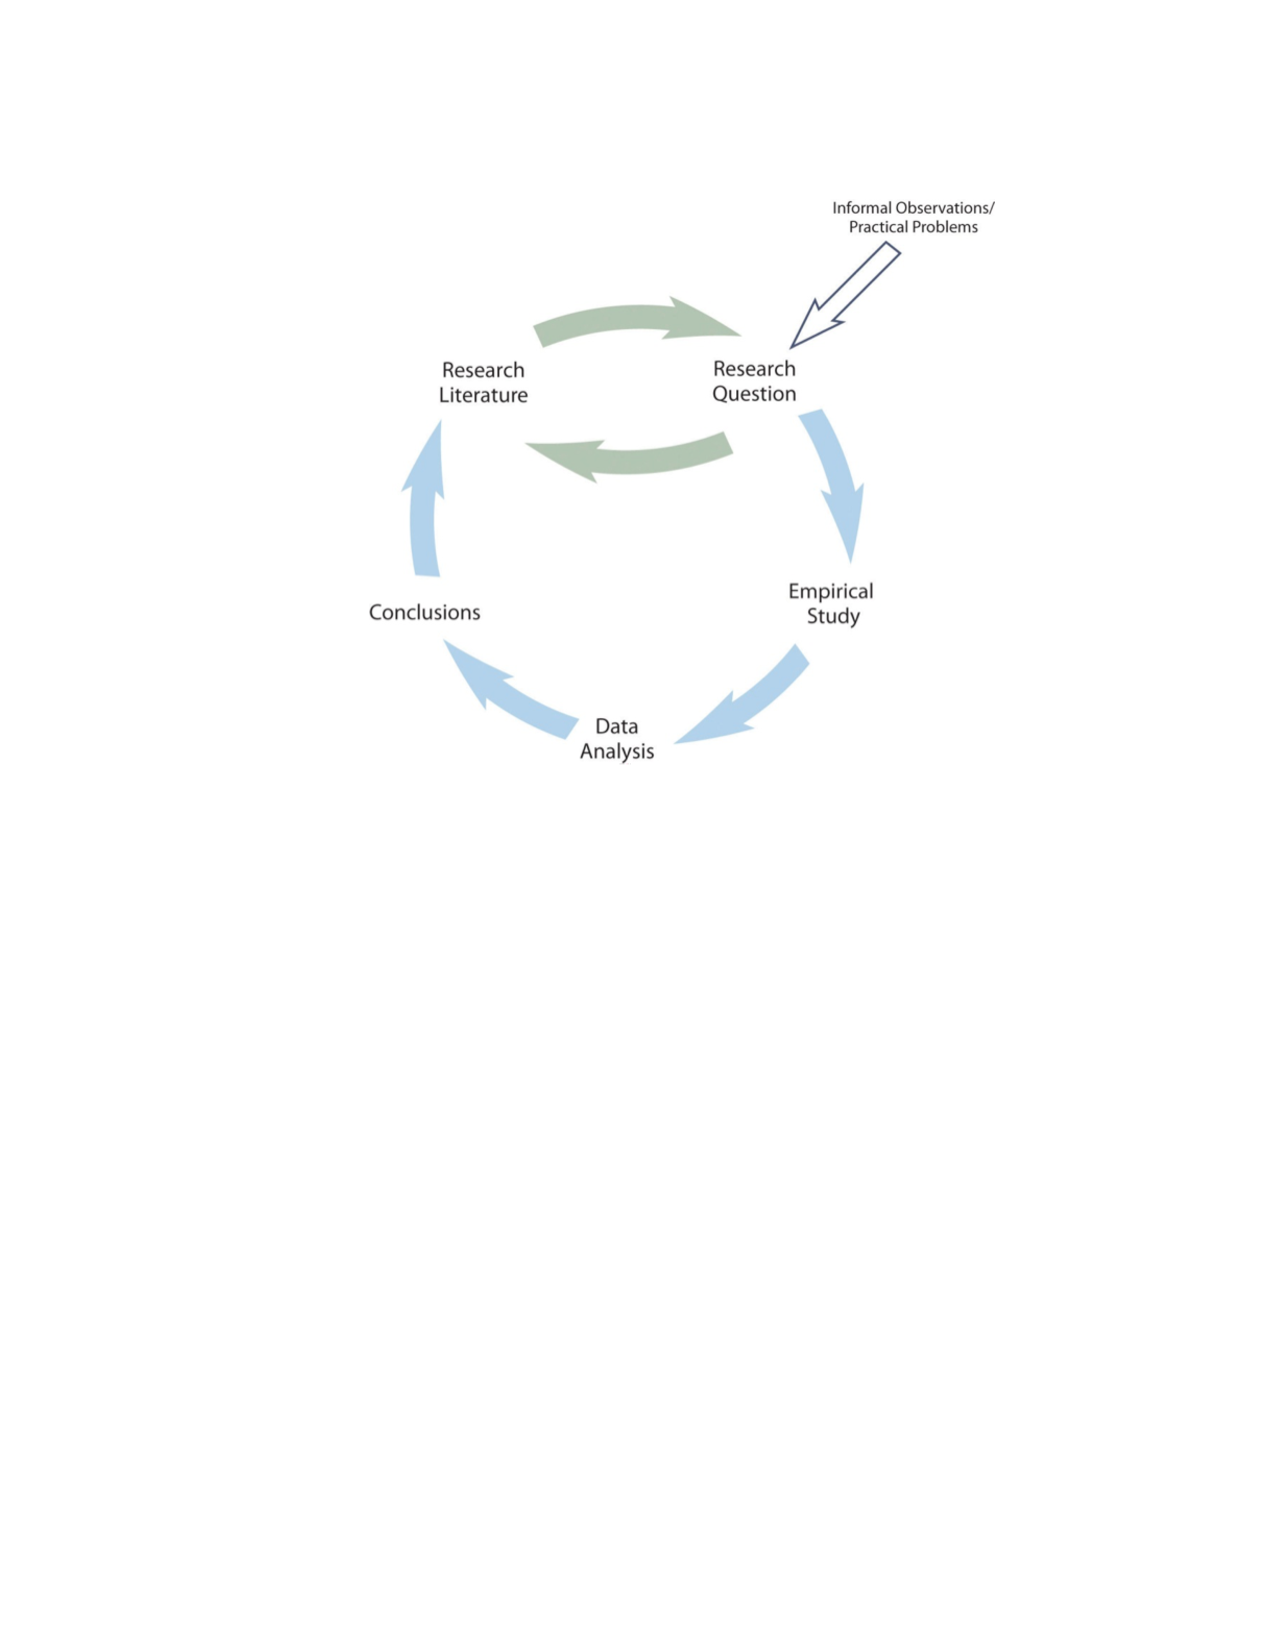
\includegraphics[width=\linewidth]{figures/C1Figure1.pdf}
      \caption{A simple model of scientific research in Psychology}
      \label{fig:Theresearchcycle}
\end{marginfigure}

Figure \ref{fig:Theresearchcycle} presents a more specific model of scientific research in psychology. The researcher (who more often than not is really a small group of researchers) formulates a research question, conducts a study designed to answer the question, analyzes the resulting data, draws conclusions about the answer to the question, and publishes the results so that they become part of the research literature. Because the research literature is one of the primary sources of new research questions, this process can be thought of as a cycle. New research leads to new questions, which lead to new research, and so on. Figure \ref{fig:Theresearchcycle} also indicates that research questions can originate outside of this cycle either with informal observations or with practical problems that need to be solved. But even in these cases, the researcher would start by checking the research literature to see if the question had already been answered and to refine it based on what previous research had already found.

The research by Mehl and his colleagues is described nicely by this model. Their question---whether women are more talkative than men---was suggested to them both by people's stereotypes and by published claims about the relative talkativeness of women and men. When they checked the research literature, however, they found that this question had not been adequately addressed in scientific studies. They then conducted a careful empirical study, analyzed the results (finding very little difference between women and men), and published their work so that it became part of the research literature. The publication of their article is not the end of the story, however, because their work suggests many new questions (about the reliability of the result, about potential cultural differences, etc.) that will likely be taken up by them and by other researchers inspired by their work.

As another example, consider that as cell phones became more widespread during the 1990s, people began to wonder whether, and to what extent, cell phone use had a negative effect on driving. Many psychologists decided to tackle this question scientifically (Collet, Guillot, \& Petit, 2010). It was clear from previously published research that engaging in a simple verbal task impairs performance on a perceptual or motor task carried out at the same time, but no one had studied the effect specifically of cell phone use on driving. Under carefully controlled conditions, these researchers compared people's driving performance while using a cell phone with their performance while not using a cell phone, both in the lab and on the road. They found that people's ability to detect road hazards, reaction time, and control of the vehicle were all impaired by cell phone use. Each new study was published and became part of the growing research literature on this topic.

\subsection{Who Conducts Scientific Research in Psychology?}

\marginnote{\allcaps{Scientific Psychology Blogs}

A fun and easy way to follow current scientific research in psychology is to read any of the many excellent blogs devoted to summarizing and commenting on new findings. Among them are the following:
\begin{itemize}
\item Brain Blogger \url{http://brainblogger.com/}
\item Mind Hacks \url{http://mindhacks.com/}
\item Research Digest \url{http://digest.bps.org.uk/}
\item Talk Psych \url{http://www.talkpsych.com/}
\item PsyBlog \url{http://www.spring.org.uk}
\item Social Psychology Eye \url{http://socialpsychologyeye.wordpress.com}
\item We're Only Human \url{http://www.psychologicalscience.org/onlyhuman}
\item You can also browse to \url{http://www.researchblogging.org}
\end{itemize}
}

Scientific research in psychology is generally conducted by people with doctoral degrees (usually the doctor of philosophy, PhD) and master's degrees in psychology and related fields, often supported by research assistants with bachelor's degrees or other relevant training. Some of them work for government agencies (e.g., the National Institute of Health), national associations (e.g., the American Psychological Association), nonprofit organizations (e.g., the Canadian Mental Health Association), or in the private sector (e.g., in product development). However, the majority of them are college and university faculty, who often collaborate with their graduate and undergraduate students. Although some researchers are trained and licensed as clinicians---especially those who conduct research in clinical psychology---the majority are not. Instead, they have expertise in one or more of the many other subfields of psychology: behavioral neuroscience, cognitive psychology, developmental psychology, personality psychology, social psychology, and so on. Doctoral-level researchers (post-doctoral fellows or research scientists) might be employed to conduct research full-time or, like many college and university faculty members, to conduct research in addition to teaching classes and serving their institution and community in other ways.

Of course, people also conduct research in psychology because they enjoy the intellectual and technical challenges involved and the satisfaction of contributing to scientific knowledge of human behavior. You might find that you enjoy the process too. If so, your college or university might offer opportunities to get involved in ongoing research as either a research assistant or a participant. 

\marginnote{Many undergraduates at Brooklyn College volunteer in research labs in the Psychology Department, and can get course credit for their work by taking Independent Study or Research courses.}

Of course, you might find that you do not enjoy the process of conducting scientific research in psychology. But at least you will have a better understanding of where scientific knowledge in psychology comes from, an appreciation of its strengths and limitations, and an awareness of how it can be applied to solve practical problems in psychology and everyday life.

\subsection{The Broader Purposes of Scientific Research in Psychology}
People have always been curious about the natural world, including themselves and their behavior (in fact, this is probably why you are studying psychology in the first place). Science grew out of this natural curiosity and has become the best way to achieve detailed and accurate knowledge. Keep in mind that most of the phenomena and theories that fill psychology textbooks are the products of scientific research. In a typical introductory psychology textbook, for example, one can learn about specific cortical areas for language and perception, principles of classical and operant conditioning, biases in reasoning and judgment, and people's surprising tendency to obey those in positions of authority. And scientific research continues because what we know right now only scratches the surface of what we can know.

Scientific research is often classified as being either \emph{basic} or \emph{applied}. Basic research in psychology is conducted primarily for the sake of achieving a more detailed and accurate understanding of human behavior, without necessarily trying to address any particular practical problem. The research of Mehl and his colleagues falls into this category. Applied research is conducted primarily to address some practical problem. Research on the effects of cell phone use on driving, for example, was prompted by safety concerns and has led to the enactment of laws to limit this practice. Although the distinction between basic and applied research is convenient, it is not always clear-cut. For example, basic research on sex differences in talkativeness could eventually have an effect on how marriage therapy is practiced, and applied research on the effect of cell phone use on driving could produce new insights into basic processes of perception, attention, and action.

\subsection{Key Takeaways}
\begin{fullwidth}
\begin{itemize}
\item Research in psychology can be described by a simple cyclical model. A research question based on the research literature leads to an empirical study, the results of which are published and become part of the research literature.
\item Scientific research in psychology is conducted mainly by people with doctoral degrees in psychology and related fields, most of whom are college and university faculty members. They do so for professional and for personal reasons, as well as to contribute to scientific knowledge about human behavior.
\item Basic research is conducted to learn about human behavior for its own sake, and applied research is conducted to solve some practical problem. Both are valuable, and the distinction between the two is not always clear-cut.
\end{itemize}
\end{fullwidth}

\subsection{Exercises}
\begin{fullwidth}
\begin{enumerate}
\item Practice: Find a description of an empirical study in a professional journal or in one of the scientific psychology blogs. Then write a brief description of the research in terms of the cyclical model presented here. One or two sentences for each part of the cycle should suffice.
\item Practice: Based on your own experience or on things you have already learned about psychology, list three basic research questions and three applied research questions of interest to you.
\item Watch the following TED Ed video \url{https://youtu.be/ GUpd2HJHUt8}, in which David H. Schwartz provides an introduction to two types of empirical studies along with some methods that scientists use to increase the reliability of their results.
\end{enumerate}
\end{fullwidth}

\newpage
\section{Science and Common Sense}

\marginnote{
\allcaps{Learning Objectives}
\begin{enumerate}
\item Explain the limitations of common sense when it comes to achieving a detailed and accurate understanding of human behavior.
\item Give several examples of common sense or folk psychology that are incorrect.
\item Define skepticism and its role in scientific psychology.
\end{enumerate}
}

\subsection{Can We Rely on Common Sense?}
Some people wonder whether the scientific approach to psychology is necessary. Can we not reach the same conclusions based on common sense or intuition? Certainly we all have intuitive beliefs about people's behavior, thoughts, and feelings---and these beliefs are collectively referred to as folk psychology. Although much of our folk psychology is probably reasonably accurate, it is clear that much of it is not. For example, most people believe that anger can be relieved by "letting it out"---perhaps by punching something or screaming loudly. Scientific research, however, has shown that this approach tends to leave people feeling more angry, not less (Bushman, 2002). Likewise, most people believe that no one would confess to a crime that he or she had not committed, unless perhaps that person was being physically tortured. But again, extensive empirical research has shown that false confessions are surprisingly common and occur for a variety of reasons (Kassin \& Gudjonsson, 2004). There are many more examples where our own intuitions about ourselves and others are incorrect.

\subsection{How Could We Be So Wrong?}

\marginnote{
\allcaps{Common Myths}

In 50 Great Myths of Popular Psychology, psychologist Scott Lilienfeld and colleagues (Lilienfeld, Lynn, Ruscio, \& Beyerstein, 2010) discuss several widely held commonsense beliefs about human behavior that \emph{scientific research has shown to be incorrect}. Here is a short list:

\begin{itemize}
\item People use only 10\% of their brain power.
\item Most people experience a midlife crisis in their 40's or 50's."
\item Students learn best when teaching styles are matched to their learning styles."
\item Low self-esteem is a major cause of psychological problems."
\item Psychiatric admissions and crimes increase during full moons.
\end{itemize}
}

How can so many of our intuitive beliefs about human behavior be so wrong? Notice that this is an empirical question, and it just so happens that psychologists have conducted scientific research on it and identified many contributing factors (Gilovich, 1991). One is that forming detailed and accurate beliefs requires powers of observation, memory, and analysis to an extent that we do not naturally possess. It would be nearly impossible to count the number of words spoken by the women and men we happen to encounter, estimate the number of words they spoke per day, average these numbers for both groups, and compare them---all in our heads. This is why we tend to rely on mental shortcuts (what psychologists refer to as heuristics) in forming and maintaining our beliefs. For example, if a belief is widely shared---especially if it is endorsed by "experts"---and it makes intuitive sense, we tend to assume it is true. This is compounded by the fact that we then tend to focus on cases that confirm our intuitive beliefs and not on cases that dis-confirm them. This is called \emph{confirmation bias}. For example, once we begin to believe that women are more talkative than men, we tend to notice and remember talkative women and silent men but ignore or forget silent women and talkative men. We also hold incorrect beliefs in part because it would be nice if they were true. For example, many people believe that calorie-reducing diets are an effective long- term treatment for obesity, yet a thorough review of the scientific evidence has shown that they are not (Mann et al., 2007)5. People may continue to believe in the effectiveness of dieting in part because it gives them hope for losing weight if they are obese or makes them feel good about their own "self-control" if they are not.

\marginnote{\allcaps{Cognitive Biases}
Psychologists have identified numerous biases that influence how people think, reason, and make judgments about the world around them. Wikipedia maintains a long list of these biases that you can check out here: \url{https://en.wikipedia.org/wiki/List_of_cognitive_biases}
}

Scientists---especially psychologists---understand that they are just as susceptible as anyone else to intuitive but incorrect beliefs. This is why they cultivate an attitude of \emph{skepticism}. Being skeptical does not mean being cynical or distrustful, nor does it mean questioning every belief or claim one comes across (which would be impossible anyway). Instead, it means pausing to consider alternatives and to search for evidence---especially systematically collected empirical evidence---when there is enough at stake to justify doing so. For example, imagine that you read a magazine article claiming that giving children a weekly allowance is a good way to help them develop financial responsibility. This is an interesting and potentially important claim (especially if you have children of your own). Taking an attitude of skepticism, however, would mean pausing to ask whether it might be instead that receiving an allowance merely teaches children to spend money---perhaps even to be more materialistic. Taking an attitude of skepticism would also mean asking what evidence supports the original claim. Is the author a scientific researcher? Is any scientific evidence cited? If the issue was important enough, it might also mean turning to the research literature to see if anyone else had studied it. Then, you could evaluate the existing evidence yourself to determine whether the evidence supports the claim.

Because there is often not enough evidence to fully evaluate a belief or claim, scientists also cultivate a tolerance for uncertainty. They accept that there are many things that they simply do not know. For example, it turns out that there is no scientific evidence that receiving an allowance causes children to be more financially responsible, nor is there any scientific evidence that it causes them to be materialistic. Although this kind of uncertainty can be problematic from a practical perspective---for example, making it difficult to decide what to do when our children ask for an allowance---it is exciting from a scientific perspective. If we do not know the answer to an interesting and empirically testable question, science, and perhaps even you as a researcher, may be able to provide the answer.

\subsection{\allcaps{Key Takeaways}}
\begin{fullwidth}
\begin{itemize}
\item People's intuitions about human behavior, also known as folk psychology, often turn out to be wrong. This is one primary reason that psychology relies on science rather than common sense.
\item Researchers in psychology cultivate certain critical-thinking attitudes. One is skepticism. They search for evidence and consider alternatives before accepting a claim about human behavior as true. Another is tolerance for uncertainty. They withhold judgment about whether a claim is true or not when there is insufficient evidence to decide.
\end{itemize}
\end{fullwidth}

\subsection{\allcaps{Exercises}}
\begin{fullwidth}
\begin{enumerate}
\item Practice: For each of the following intuitive beliefs about human behavior, list three reasons that it might be true and three reasons that it might not be true:
\begin{itemize}
\item You cannot truly love another person unless you love yourself.
\item People who receive "crisis counseling" immediately after experiencing a traumatic event are better able to cope with that trauma in the long term.
\item Studying is most effective when it is always done in the same location.
\end{itemize}
\item Watch the following video, in which psychologist Scott Lilienfeld talks about confirmation bias, tunnel vision, and using evidence to evaluate the world around us \url{https://youtu.be/ Eut8jMfSA_k}
\end{enumerate}
\end{fullwidth}

\newpage
\section{Science and Clinical Practice}

\marginnote{\allcaps{Learning Objectives}

\begin{enumerate}
\item Define the clinical practice of psychology and distinguish it from the science of psychology. 
\item Explain how science is relevant to clinical practice.
\item Define the concept of an empirically supported treatment and give some examples.
\end{enumerate}
}

Psychology is the scientific study of behavior and mental processes. But it is also the application of scientific research to "help people, organizations, and communities function better" (American Psychological Association, 2011). By far the most common and widely known application is the clinical practice of psychology---the diagnosis and treatment of psychological disorders and related problems. Let us use the term clinical practice broadly to refer to the activities of clinical and counseling psychologists, school psychologists, marriage and family therapists, licensed clinical social workers, and others who work with people individually or in small groups to identify and help address their psychological problems. It is important to consider the relationship between scientific research and clinical practice because many students are especially interested in clinical practice, perhaps even as a career.

\marginnote{\allcaps{Empirically Supported Treatments}

An empirically supported treatment is one that has been studied scientifically and shown to result in greater improvement than no treatment, a placebo, or some alternative treatment. These include many forms of psychotherapy, which can be as effective as standard drug therapies. Among the forms of psychotherapy with strong empirical support are the following:

\begin{itemize}
\item Cognitive behavioral therapy. For depression, panic disorder, bulimia nervosa, and post- traumatic stress disorder.
\item Exposure therapy. For post-traumatic stress disorder.
\item Behavioral therapy. For depression.
\item Behavioral couples therapy. For alcoholism and substance abuse.
\item Exposure therapy with response prevention. For obsessive-compulsive disorder.
\item Family therapy. For schizophrenia.
\end{itemize}

For a more complete list, see the following website, which is maintained by Division 12 of the American Psychological Association, the Society for Clinical Psychology  \url{http://www.div12.org/psychological- treatments}

}

The main point is that psychological disorders and other behavioral problems are part of the natural world. This means that questions about their nature, causes, and consequences are empirically testable and therefore subject to scientific study. As with other questions about human behavior, we cannot rely on our intuition or common sense for detailed and accurate answers. Consider, for example, that dozens of popular books and thousands of websites claim that adult children of alcoholics have a distinct personality profile, including low self-esteem, feelings of powerlessness, and difficulties with intimacy. Although this sounds plausible, scientific research has demonstrated that adult children of alcoholics are no more likely to have these problems than anybody else (Lilienfeld et al., 2010). Similarly, questions about whether a particular psychotherapy is effective are empirically testable questions that can be answered by scientific research. If a new psychotherapy is an effective treatment for depression, then systematic observation should reveal that depressed people who receive this psychotherapy improve more than a similar group of depressed people who do not receive this psychotherapy (or who receive some alternative treatment). Treatments that have been shown to work in this way are called \textbf{empirically supported treatments}.

Many in the clinical psychology community have argued that their field has not paid enough attention to scientific research---for example, by failing to use empirically supported treatments---and have suggested a variety of changes in the way clinicians are trained and treatments are evaluated and put into practice. Others believe that these claims are exaggerated and the suggested changes are unnecessary (Norcross, Beutler, \& Levant, 2005). On both sides of the debate, however, there is agreement that a scientific approach to clinical psychology is essential if the goal is to diagnose and treat psychological problems based on detailed and accurate knowledge about those problems and the most effective treatments for them. So not only is it important for scientific research in clinical psychology to continue, but it is also important for clinicians who never conduct a scientific study themselves to be scientifically literate so that they can read and evaluate new research and make treatment decisions based on the best available evidence.

\subsection{\allcaps{Key Takeaways}}
\begin{fullwidth}
\begin{itemize}
\item The clinical practice of psychology—the diagnosis and treatment of psychological problems—is one important application of the scientific discipline of psychology.
\item Scientific research is relevant to clinical practice because it provides detailed and accurate knowledge about psychological problems and establishes whether treatments are effective.
\end{itemize}
\end{fullwidth}

\subsection{\allcaps{Exercises}}
\begin{fullwidth}
\begin{enumerate}
\item Discussion: Some clinicians argue that what they do is an “art form” based on intuition and personal experience and therefore cannot be evaluated scientifically. Write a paragraph about how satisfied you would be with such a clinician and why from each of three perspectives:
\begin{itemize}
\item a potential client of the clinician
\item a judge who must decide whether to allow the clinician to testify as an expert witness in a child abuse case
\item an insurance company representative who must decide whether to reimburse the clinician for his or her services
\end{itemize}
\item Practice: Create a short list of questions that a client could ask a clinician to determine whether he or she pays sufficient attention to scientific research.
\end{enumerate}
\end{fullwidth}

\section{Using Psychological Science to Inform Your Worldview}

Psychology is a very broad scientific discipline that asks and answers all sorts of questions about human and non-human animals. Psychological science encompasses many levels of analysis spanning the building blocks of biological systems, such as genes and cells, neurochemistry, neurons, and networks of neurons; perceptual and cognitive abilities of individuals such as learning, memory, attention, decision-making, language, thought, intelligence, and consciousness, to complex aspects of individuals such as development, personality, social behavior, and many others. A typical introductory psychology has the difficult job of presenting a bird's eye view of all of these major psychological domains of inquiry. Although psychologists ask many different kinds of questions, they all employ the scientific method as a tool to answer questions. So, this course is an introduction to the scientific research methods that are used in all areas of Psychology.

The primary focus of the course will be on experiments, which is the most powerful empirical tool researchers have to determine the underlying causes of the psychological phenomena that they measure. Psychological research methods are not limited to experiments, and non-experimental, or quasi-experimental approaches are often used with great success to ask and answer questions. Some of these research methods will be highlighted throughout the course.

\subsection{Why Should I Care About How Psychology Experiments work?}

Imagine for the moment a world without experiments that does not use the scientific method. This world would still have people claiming to have knowledge about how things work, and it would still have tools and technologies that are claimed to solve particular problems. However, without experiments to test whether the claims are true, all we are left with is the untested claims that may be true or false. We would be left in the dark. Inevitably, and not too different from our world today, there would be large segments of the population who believe false claims about how things work, and large segments of the population using therapies, tools, or other technologies that simply do not work (even if they believe they do).

The world we live in today discovered the scientific method and uses experiments to test claims about how things work. Indeed, with the enormous number of ways that we receive information through the media today, it is difficult to avoid hearing about all sorts of new scientific claims as well as totally unfounded claims that may not be based in science. For example, we have probably all heard that eating too much of something is good or bad for you, and increases or decreases your risk for a health problem. These claims can even flip around so that last year eating too much of X was bad, but this year eating too little of X is bad. What's more, many of these claims are supposedly scientific ones based on experiments. Should you believe these claims, and should you change your own behavior because of them?

 When we receive claims through the media we are getting second-hand information, and based on this information alone it is difficult to evaluate the claim and the evidence for the claim. One option is to find expert reporters that you trust, and then believe everything they say. The second option is to find the primary source, and then evaluate the evidence yourself to determine whether you should believe the claim. The ability to understand how experiments work gives you the tools you need to critically evaluate claims about how things work.

\subsection{Evaluating Claims}

It is an understatement to say that people believe all sorts of crazy things. Note, this is a claim that I just made. Should you believe it? What do you need to know to determine whether or not you should believe this claim or any other claim? Scientific thinking requires that claims are supported by evidence. Other forms of belief and thinking may not require evidence to support claims. 

For the moment I'll put on my scientific thinking hat because there numerous ways that I can provide evidence for my claim the people believe all sorts of crazy things. I am a person, and I know that I have believed crazy things in the past. For example, when I was four I believed that all children grow to be taller than their parents because I visited a family who had many children of different ages, and the oldest ones were all taller than their parents. I believed this claim for many years until finding out at the age of 12 that all of the children in that family were adopted (nevertheless, I am taller than both my parents, but my brother is not, so much for my theory). The internet is full of people claiming to believe things that I think are completely crazy. For example, the flat earth society believes that the earth is flat and shaped like a frisbee. Believers in the great reptilian conspiracy maintain that many of our world leaders are lizard people. The abundance of conspiracy theories provides a deep well of evidence that people believe all sorts of crazy things. So, because I can back up my claim with evidence, I will continue believing that people believe all sorts of crazy things. 

I could also take my science hat off, and then I can believe anything I want. Indeed, this remarkable imagination ability may be one reason why people believe so many crazy things without needing any evidence whatsoever to back up their beliefs. I can believe that I am a lizard monster who lives on a frisbee just because I want to. Indeed, the freedom to have your own opinion or belief about anything is a sacred cultural value in our western democracy. As citizens we respect each others right to their own opinions and beliefs. This is a way of respecting the right to have truthful and false and crazy beliefs, or respecting each others right to be completely wrong.   

\subsection{Testable and Untestable Claims}
The scientific method for determining whether claims are true or false, or somewhere in the middle, has limitations because it can only be used to evaluate testable claims. A testable claim is one that makes a clear implication about a state of the world. For example, I claim that I have two hands. This is a testable claim because it clearly implies that if someone were to observe my arms, they would expect to find two hands at the end of them. If they did not find two hands, then they could dispatch with my claim because the evidence showed I had no hands, which would be in direct contradiction with the claim. An untestable claim is nonsensical, or does not make a clear implication about a state of the world. For example, consider the claim “aldfoha ofghnfsklhjas asdfilubhs”. This is just nonsense, and no one knows what it means, it does not make clear implications about a state of the world, so we will never know if it is true or false. Consider the claim “the members of the Zarkovian alien race from planet Zarko in a parallel universe all look like perfect glass spheres”. This claim is possibly sensical, because it could be tested if we could travel to that planet and find members of the Zarkovian race, but it is not practically testable because the needed evidence can not be gathered; so, we will never know if this made up claim is true or false, or almost true (perhaps they are cubes or ellipsoids).

Claims and evidence are two central parts of the scientific method. And, in psychological science neither of these parts come for free. Researchers construct both of them. One job is to create claims that can be tested. The other job is to make the evidence by creating situations necessary to conduct the tests. Joining the creation of claims with the creation of testable situations produces evidence that bears directly on the claim. The evidence can be consistent or inconsistent with the claim, allowing the claim to continue to be accepted or rejected. 

Here is another claim: People don't always like to be wrong. I don't always like to be wrong, so at least there is one example. People have beliefs that are near and dear to their heart, so close perhaps, that a person might be completely devastasted if they found out one of their precious ideas was wrong. For this reason, the evidence provided by scientific research may be viewed as a threat to a persons system of beliefs about the world. After all, when those beliefs involve testable claims, research can sometimes show those claims to be competely false. In which case, a rational person might be forced to delete parts of their beliefs that they would have preferred to hold on to. However, people aren't always rational and discovering evidence does not force anyone to do anything. For example, lots of research shows that people can persevere in maintaining false beliefs, even after they are told about the evidence showing their beliefs are false. So, people really do believe crazy things.

\subsection{Learning How Not To Be Crazy}
Learning about how experiments work is an opportunity to learn how not be crazy. Remember, experiments can only tell us about claims that can be tested, so we can not use this method to know whether our untestable beliefs are crazy. Fortunately, there are an endless number of testable claims that we can investigate that can add to the evergrowing library of human knowledge that science has produced so far, and be translated to applications that benefit ourselves, society, and the world around us. 



\chapter{1 Overview}
\lhead{\allcaps{Overview}}

\openepigraph{Today was good. Today was fun. Tomorrow is another one.}{---Dr. Seuss}

\section{General Overview}

The weekly labs are structured to give students experience with conducting experiments, analyzing data, thinking critically about theory and data, and communicating their results and analysis in writing and oral presentation. 

Lab instructors facilitate this process by guiding students through the demands of each of the labs. Lab instructors are there to help you, so ask them questions when you need answers!

\subsection{Lab structure: Major and mini projects, and presentations}

The entire semester is divided into three major projects, and 3 mini projects. They are ordered consecutively to build upon skills. For example, the first projects focus on data analysis skills involving t-tests, then one-way ANOVAs, and finally 2x2 Factorial designs. Throughout each of the labs you will learn how to create experiments and conducts analyses on the data. Then you will employ these skills in the last half of the semester when you form groups and conduct, analyze, report and present an experiment of your own design.


\subsection{Major projects}  

Each major project involves students completing an experiment as a class (using themselves as subjects to collect data). Students will learn about the conceptual issues behind the experiment, collect data on themselves, and analyze the class data using appropriate statistics. Each student will then be responsible for writing a short (5+ page) APA style report about the project. 

The first two major projects involve predefined experiments that the class completes. These two projects are roughly finished mid-semester, and are intended to train students in the skills needed to complete the final project. The last major project is the final project, where students form groups and complete an experiment based on their own design. 

Each lab instructor is responsible for grading each of their students papers. Individual lab instuctors will explain to their sections how their grading scheme will work.
 
\subsection{Mini projects} 
In the first half of the semester, each of the weeks that does not introduce a new major project are reserved for mini-projects. These projects are intended to be completed within one lab session. Each of the mini-projects involve 1) reading and understanding a primary source, and 2) attempting to replicate the result in the paper. These are graded on a pass/fail basis, where a pass is given to students who show up and participate in the lab (regardless of whether their experiment turns out.)

\subsection{Presentations} 
The final project involves two presentations. An individual presentation, and a group presentation. Prior to forming groups for the final project, each student will give a short (2-3) minute pitch for their project idea. Then, students will form groups (choose one of the members project ideas, or generate a new one) and begin working on their final project. The last lab is reserved for the group presentations where each group gives a 10 minute research presentation. 

\subsection{Grading}

Each lab instructor will grade the work of the students in their sections. See the course syllabus for information on how each of the lab components weigh into the final grade for the course.

\section{Lab Resources}

There are many resources to help you complete the lab assignments. These are included in this lab manual, as well as online.

\subsection{Website}

As much as possible all of the information for this course will be posted on the course website:

\url{http://crumplab.github.io/courses/experimental/}

\subsection{Lab rooms} 

There should be one computer per student in each of the lab rooms. These computers should have SPSS, Excel, Office, R, Superlab, LIVECODE, and Psychopy installed on them. 

\subsection{Lab manual} 

This lab manual contains instructions for each the lab assignments, as well as helpful tutorials for learning skills to analyze and report data.

\section{Lab Schedule}

\subsection{Lab 1: Overview}
\begin{enumerate}
\item Meet and greet your instructor and fellow classmates, and learn about what is in store for the labs this semester	

a.	You will write three APA style research reports. Papers 1 and 2 will be on predefined projects, and Paper 3 will be based on a final project where students form groups to complete an experiment of their own design

b.	The final project will involve two presentations, an individual presentation and a group presentation. 

c.	The first half of the semester involves completing Papers 1 and 2, and a few mini-projects that occur between papers 1 and 2. These will build the skills necessary to complete the final project which will take up most of the second half of the semester
\item	Students are expected to show up and be on time for labs
\item	Ask questions
%\item	Administer Confidence in Reading Primary sources Questionnaire
%
%a.	Explain that part of the lab and lecture curriculum is designed to help students build skills in reading primary source material, and that we will be conducting some research to assess these outcomes. 
%
%b.	Give verbal consent procedure
%
%c.	Hand out questionnaires (10 minutes), collect them and return them to Nick Brosowsky’s mailbox in the main office.
\item	Go over QALMRI method using provided QALMRI materials
\item	Discuss/Review the components of writing an APA paper
\end{enumerate}

\subsection{Lab 2: Paper project 1}

Students replicate the results of \citeauthor{song_if_2008} (2008)\cite{song_if_2008}.

\begin{enumerate}
\item Administer the experiment using the provided materials

a.	Students will receive a piece of paper with instructions. They will read the description of an exercise routine, and then answer the questions about what they read.
\item	Reading and understanding the primary source

a.	Students will be given the Song \& Schwarz (2008) paper, and the to-be-filled in QALMRI worksheet. They will be given 15-20 minutes to read the paper, and in small groups attempt to fill out the QALMRI worksheet for the paper

b.	Group discussion of the paper and the QALMRI
\item	Collect and analyze the data
\item	Discuss the paper assignment
\end{enumerate}

\subsection{Lab 3: Paper project 1 continued}
\begin{enumerate}
\item More time to work on the first paper. Use your lab instructor as a resource and ask questions if you need more info.

E.g., Review APA style, review the structure and content of the paper, review the results, edit each others work, etc.
\item Due dates are set by the lab instructor
\end{enumerate}

\subsection{Lab 4: MiniProject 1 Nairne, Pandeirada, \& Thompson (2008)}

Students replicate the results of \citeauthor{nairne_adaptive_2008} (2008)\cite{nairne_adaptive_2008}.

\begin{enumerate}
\item Students read paper and write QALMRI (15-20)
\item Group discussion about paper (15-20)
\item	Students attempt to replicate the major findings in the paper

a.	Break into four-five groups, each group assigned an encoding condition (Survival, Pleasantness, Imagery, Self-reference, Intentional learning)

b.	Each group picks their own 30 words. Can follow same procedure as in paper by choosing 30 words from Overschelde, Rawson, \& Dunlosky (2004) \cite{van_overschelde_category_2004}.

c.	Groups try to run at least 10 participants in their condition, recording proportion of correctly recalled words

d.	Groups enter their collected data into the master spreadsheet, which is given back to groups upon data completion

\item Discussion of how to analyze the data
\item Group attempt to analyze the data using t-tests and one-way ANOVA to determine if the survival framing produced better recall than the other conditions.
\end{enumerate}

\subsection{Lab 5: Mini Project 2 Stoet et al. (2013)}

Students replicate the results of Stoet et al. (2008) \cite{stoet_are_2013}.

\begin{enumerate}
\item Students read paper and write QALMRI (15-20)
\item Group discussion about paper (15-20)
\item Students download the task-switching program available from the website and individually complete the task. Individual students then enter their data in the master spreadsheet
\item Discussion of how to analyze the data. Major analysis goals are:

a.	Was there a mixing cost? Compare pure lists to mixed lists

b.	Was there a switching cost? Compare switch vs. repeat trials in pure lists

c.	Was there a gender effect?

\item Students break into groups to analyze the data.
\end{enumerate}

\subsection{Lab 6: Mini Project 4 Raz et al. (2006)}
Students replicate the results of Raz et al. (2006) \cite{raz_suggestion_2006}
\begin{enumerate}
\item Students read paper and write QALMRI (15-20)
\item	Group discussion about paper (15-20)
\item	Students instructed their task is create their own Stroop design and employ a manipulation that increases or decreases the size of the Stroop effect
\item	Students break into groups and conduct a Stroop experiment, measuring the size of the Stroop effect in a "normal" condition, and in their manipulated condition.
\item	Groups analyze conduct a 2x2 ANOVA to see if their interaction was significant
\end{enumerate}


\subsection{Lab 7 : Paper Project 2 Yin (1969)}
Students replicate the results of Yin (1969) \cite{yin_looking_1969}
\begin{enumerate}
\item Students read paper and write QALMRI (15-20)
\item	Group discussion about paper (15-20)
\item	Students complete computerized task and report their data in the master spreadsheet. Data is given back to students for analysis
\item	Discussion about writing the 2nd paper
\end{enumerate}

\subsection{Lab 8: Paper project 2 continued}
\begin{enumerate}
\item Extra-time for completing second paper, again use your lab instructor as a resource, they are there to help.
\end{enumerate}


\subsection{Lab 9: Brainstorming for Final project}

\begin{enumerate}
\item Learn about details of the final project
\item Learn about details of the individual presentation (next lab)
\item Brainstorming session allowing students to think about possible projects that they would propose for their individual project
\end{enumerate}

\subsection{Lab 10: Individual Presentations}
\begin{enumerate}
\item Students give their individual (2-3 minute) presentations
\item Students are divided into groups for their final project
\item Each group decides on the experiment for their final project. This could be from one of the individual project ideas, or a new idea. Groups need permission from the lab instructor for their final project before data collection begins
\end{enumerate}

\subsection{Lab 11-13: Group work on Final Project}
\begin{enumerate}
\item Help groups finalize their final project aims
\item Groups collect data
\item Discuss requirements for final presentation and paper
\end{enumerate}

\subsection{Lab 14: Final group presentations}



\chapter{2 The QALMRI Method}
\lhead{\allcaps{The QALMRI Method}}

\openepigraph{Question Alternatives Logic Method Results Inference}{---The QALMRI Method}

The general goal of this course is to give you experience with the scientific process of asking and answering psychological questions. At the end of the course you should gain at least two kinds of skills. First, in the labs you will learn to ask and answer your own questions by conducting, analyzing, and reporting the results of experiments that you conduct. Second, you learn how understand the research literature, where other researchers have asked and answered questions, and communicated them publicly by publishing journal articles on their research.

There are a lot of details involved in asking and answering questions in science, and you can easily see these details on display by reading any published peer-review journal article. You will become very familiar these details as you read more papers, and as you write your own APA style research reports.

The details can be daunting, mainly because the format and structure of articles may be unfamiliar, and the language that scientists use is often very specific (or jargony). As a result, if you are not already an expert in a particular domain, it can be very difficult to read and understand research presented in journal articles. Furthermore, if you do not understand the concepts behind the questions, and the details behind the methods and results, then it is difficult to write your own research reports about experiments that you conduct. Have no fear, this lab manual is here to guide you through the process. 

Ultimately, by learning the skills we teach you throughout this semester, you will be able to critically evaluate your own research, as well as the research literature at large. This will allow you form your own opinions about the process of asking and answering questions. For example, when you learn how to critically evaluate research you will be able to:
 
\begin{enumerate}
\item Evaluate whether or not you should believe particular scientific claims, or claims made by the media about new "research findings"
\item Look at the evidence to see whether it actually provides an answer to the question that was being asked
\item Look at the questions to see if they are good ones, and learn how to ask better questions
\item Understand how theories and hypotheses work and make predictions about psychological phenomena
\item Learn how to find scientific research that has been conducted on topics of your own interest, and then evaluate the claims and evidence for yourself. For example, the skills you learn here about evaluating psychological research are the same skills that you would need to evaluate medical research. So, if you are wondering whether a particular medical procedure, or drug, or diet works or doesn't work, then you can read the research for yourself to arrive at your own informed opinion.
\end{enumerate}

\section{The QALMRI Method}

The first step is learning how to read journal articles. We will use the QALMRI method throughout this course as a tool to help you identify the major ideas and findings presented in journal articles. The major aspects of the QALMRI method will also help you identify whether your own research reports contain the information necessary to communicate your own research. First, we will explain the QALMRI method, then we will explain how you will be asked to use it throughout the course.

\marginnote{Adapted nearly verbatim from: Kosslyn, S.M. \& Rosenberg, R.S. (2001). Psychology: The Brain, The Person, The World. Boston: Allyn \& Bacon.}

The QALMRI method provides a means for critically evaluating experiments, as well as for organizing your own experiment proposals. It helps you to find connections between theory and data by making explicit the question being asked, the approach used to answer it, and the implications of the answer. QALMRI is an acronym, and each letter identifies critical parts of research articles.

\subsection{Q stands for Question}

All research begins with a question, and the point of the research is to answer it. For example, we can ask whether a placebo is better than no action in alleviating depression. For most journal articles, the General Introduction should tell the reader what question the article is addressing, and why it is important enough that anyone should care about the answer. Questions fall into two categories: broad and specific. In your QALMRI, state both the broad and the specific questions being asked. Broad questions are typically too general to answer in a single experiment, although one should view the experiment as one step on a journey to answer the broad question. An example of a broad question might be "Does language influence perception?" This sort of question provides the general topic of the paper, and can only be answered through compiling many experimental results. In contrast, the specific question can typically be addressed in a single experiment or set of experiments. A specific question might be "If one language has a specific term for one color, and another language does not have any term for that color, will speakers of the two languages perceive the color differently?" 

Again, be sure to identify the broad and specific question relevant to your data collection. 

\subsection{A stands for Alternatives}

Good experiments consider at least 2 possible alternative answers to a specific question, and explains why both answers are plausible. For example, the possibility that speakers of different languages will perceive colors differently is plausible based on evidence that top-down processes can affect perception. The alternative hypothesis, that language does not influence perception of color, is also plausible because color perception in particular might be impervious to top-down influences. That is, it might be based solely on properties of the visual system which are unaffected by language. When describing an existing article or when proposing an experiment, you should identify the alternatives the authors considered. There are always at least 2 alternatives: that factor X will show an effect, or that it won't (that a null result will be obtained). If possible, identify other alternative patterns as well. 

\subsection{L stands for Logic}

The logic of the study identifies how the experiment's design will allow the experimenter to distinguish among the alternatives. The logic is typically explained towards the end of the study's introduction, and has the following structure: If alternative 1 (and not alternative 2) is correct, then when a particular variable is manipulated, the participants' behavior should change in a certain way. For example, the logic of the color experiment would be: If a person's native language influences their perception of color, then speakers who have a term for a given color should respond differently to that color than speakers whose language contains no term for that color. Alternatively, if language does not influence color perception, then speakers who have a color term should respond no differently than speakers who lack the term. Note that the logic of the experiment is integrally connected to the alternatives you stated in the last section. Indeed, this section should be comprised of a series of "If, then" statements in which you restate the alternatives you offered ("If X,"), and then state what pattern of data would support that alternative ("then Y"). You should therefore have equal numbers of alternatives and If…then statements. 

\subsection{M stands for Method}

This section identifies the procedures that will be used to implement the logical design. It should state the independent variable (the factor being experimentally manipulated) and the dependent variable (the behavior being measured) of the experiment. It should also describe the subjects, including whether subjects were divided into groups receiving different experimental manipulations. What materials were used to conduct the experiment, and what were the experimental stimuli like? 

\subsection{R stands for Results}

What was the outcome of the experiment? Describe the results of the primary measures of interest. For example, did different subject groups yield different group means? What were these means? Or did the entire subject population produce a distinctive pattern of responses? Describe that pattern. Did the results seem reliable, or do you feel they might have been an artifact of the way the experiment was conducted? For this section, it is often a good idea to use graphs or tables to illustrate the pattern of data you obtained. 

\subsection{I stands for Inferences}

What can the results of the experiment tell us about the alternatives? If the study was well designed, the results should allow you to eliminate at least one of the possible alternatives. For example, if a language lacks a color word but the speakers of that language respond to the color no differently than speakers of a language lacking a term for the color, then the experiment supports the view that language does not influence color perception. At this point, take a step back and think about any potential problems with the experiment that could have led to the pattern of results you obtained. Were there confounds that could have caused the results? For example, if you did find a difference between the subject groups, are there other ways in which the groups differ that are not language-related? Might this have caused the result? Were there problems during the data collection? In addition, this is the section in which to consider the hypothetical next step in answering the broad question. If you were to conduct a follow-up experiment, what would it be (hint: think of questions that remain unanswered by the present results, and sketch a study that could bear on one or more of those questions)? What questions do your results raise? 

\section{Writing a QALMRI}

Writing a QALMRI for any research paper (one that you are writing, or one that you are reading) is simply writing short answers to each of these questions using clear and concise language. It is a condensed, short-form, version of the research. To be even more specific, your task is to answer these questions:

\marginnote{\allcaps{How long is a QALMRI?} Long-enough to answer each question with clear and brief sentences.} 

\begin{itemize}
\item Question: What was the broad question? What was the specific question?
\item Alternative hypotheses: What were the hypotheses?
\item Logic: If hypothesis 1 was true, what was the predicted outcome? What was the predicted outcome if hypothesis 2 was true?
\item Method: What was the experimental design?
\item Results: What was the pattern of data?
\item Inferences: What can be concluded about the hypotheses based on the data? What can be concluded about the specific and broad question? What are the next steps?
\end{itemize}

In many of the weekly labs you will read a primary research article, and then write your own QALMRI summary. This will help you extract the big ideas and findings from the research. You will also discuss your QALMRIs as a group to make sure that everyone is on the same page about what the research was about, and what the research showed.

\section{Example QALMRI}

Even if you haven't read the article, reading a QALMRI should provide you with enough information to get a basic idea of what the article was about. The following QALMRI summarizes the article by Crump \& Logan (2010). \cite{crump_warning:_2010}

\subsection{What was the broad and specific question?}

The broad questions are about spatial cognition. How do people understand and represent the spatial relationships between objects in the environment? Do people have "spatial maps" in their head?

The specific question is how do typists know where the keys are on the QWERTY keyboard?

\subsection{What are the alternatives?}

\begin{enumerate}
\item Typists have an internal cognitive spatial map of the keyboard that they use to guide their fingers during typing
\item Typists do not have a map-like representation, instead they rely on learned associations between cues such as the feel of the keyboard to guide their fingers during typing
\end{enumerate}

\subsection{What is the logic?}
\begin{enumerate}
\item If typists have an internal map of the keyboard, then they should be able guide their fingers to correct locations based on the map alone, and no feedback from the environment. For example, if we could measure "air-typing" without a keyboard, then typists should still be able to put their fingers in the correct locations even when the keyboard is missing because they are relying on their internal map.

\item If typists do not use an internal map of the keyboard, then their finger movements should become slow and inaccurate when they try to type without a keyboard, or in other conditions that change the normal feel of the keyboard, and thereby remove the cues that typists use to direct their fingers.
\end{enumerate}

\subsection{What is the Method?}
Typists copied paragraphs in four conditions that manipulated tactile (touching) feedback from the keyboard. They typed on a normal keyboard, a keyboard with the keys removed exposing the rubber buttons underneath, a flat circuit board without, and on a flat table with a laser projection keyboard.

\subsection{Results}

Typists were fast and accurate in the normal keyboard condition. Typists were slow and inaccurate in all of the other keyboard conditions, where normal tactile feedback was removed.

\subsection{Inference}

The results are \emph{not consistent} with the internal map hypothesis. If typists had an internal map, and did not rely on tactile cues, then they should have typed normally even when the cues were removed. The results are consistent with learned association hypothesis, that typists rely on cues, like the feel of the keyboard, that are associated with particular key locations.

\section{Finding the QALMRI sections in a journal article}

Most psychology journal articles are in APA format. See the textbook, and the sections about APA style in this lab manual for more on that format. APA format makes it relatively easy to find the sections of the QALMRI. The basic parts of an APA manuscript are 
\begin{enumerate}
\item Title - Offers clues about the big idea and finding
\item Abstract - Usually a useful summary of the whole research.
\item Introduction - Big questions are usually near the beginning, specific questions are usually in the middle. Alternatives (or Hypotheses) and Logic are usually just before the Experiment, and sometimes in the short introduction to the experiment.
\item Methods - a whole section devoted to the M part
\item Results - a whole section devoted to the R part
\item Discussion - Usually provides a summary of the main important finding right at the beginning
\item General Discussion - Should connect the main finding to the hypotheses and questions under investigation
\end{enumerate}

Most articles that are not in APA style also have very similar sections, and you should find the answers to the QALMRI in the same places. Some journals like Science and Nature have the method sections at the very end. Also, some journals have short article formats, where the research is presented in one or two pages. Oftentimes short reports do not have headers; nevertheless, the answers to the QAL parts are usually near the beginning and middle, and the answers to the RMI parts are usually near the end. 

To get some practice extracting QALMRI from a journal article, let's look at short report published in Science. We'll look at the Mehl et al. (2007) \cite{mehl_are_2007} paper, discussed in chapter 1 of the textbook. It's only one page long, so it's an easy read.

 \href{https://login.ez-proxy.brooklyn.cuny.edu/login?url=http://science.sciencemag.org/content/317/5834/82}{Click this link to get the paper online}. Note, if you are on the Brooklyn College network, this should take you directly to the paper. If you are at home, you will need to first sign into the library.

\subsection{Finding the Big Question}

You might say the big question is implied by first sentence, "Sex differences in conversational behavior have long been a topic of public and scientific interest". The big question is not stated directly, but you could infer that the questions are something like, 1) Are there sex differences in talking, or other conversational behavior?, 2) Do women talk more than men?, 3) Why do women talk more than men?, and so on. 

You might also read this article and conclude that the authors did not really spell out the big questions. After all, they only had a single page to communicate their research. So, it is important to realize that there are big questions that may not actually be stated. You, the reader, need to connect the dots. For example, we could say some of the really big questions are: 1) What are the main sex differences in communication, language, and cognition in general, 2) How do people use language to communicate, 3) What cognitive, biological, genetic, and environmental mechanisms cause sex differences in these behaviors? You can see that the research relates to these bigger questions, even if they are not explicitly stated.

\subsection{Finding the Specific question}

In this case, the specific question is hard to miss. It's in the title, "Are women really more talkative than men?". The authors motivate asking this question by pointing out that systematic research has not actually measured how many words men and women say on average per day.

\subsection{Alternatives}

The hypotheses in this article are pretty straightforward because they are clearly related to an empirical question. One hypothesis is alluded to in the second sentence, where the authors claim that western society has a stereotype that women are more talkative than men. In this case, the hypotheses in question are not about psychological processes or mechanisms, they are simply about the data. The authors also do not formally state two hypotheses. We have to do that for them.

\begin{itemize}
\item Hypothesis 1: Women are more talkative than men
\item Hypothesis 2: Women are not more talkative than men
\end{itemize}

\subsection{Logic}

In this case, the logic of the hypotheses is nearly identical to the hypotheses themselves, but simply stated in terms of a logical if/then structure.

\begin{itemize}
\item If, women are more talkative than men, then women should on average produce more words per day than men
\item If, women are not more talkative than men, then women should on average produce the same or less number of words per day than men.
\end{itemize}

\subsection{Methods}

You can see the methods described in paragraphs three and four. Basically, they recorded subjects all day long in their natural environments, and then counted how many words they said.

\subsection{Results}

The results are in paragraph six, and presented in the table. You already know the question: "Do women talk more than men?", and that they measured the number of words spoken by groups of men and women, so you should expect to find some average data showing the actual counts. We see this in the weighted average in the table. Women said on average 16,215 words per day, and men said 15,669 words per day. The results section says that this result was not statistically different, and could have easily been produced by chance. You can even see that some of the sub-groups showed the opposite pattern of data, with men saying more words per day than women.

\subsection{Inference}

The authors make inferences about their hypotheses in the last two paragraphs. Their major inference is that, contrary to popular belief, women are not more talkative than men. They also discuss some limitations of their work.

\subsection{Reading between the lines}

We saw that some parts of the QALMRI weren't explicitly stated the by authors in the manuscript. However, all of the major parts were implied by what they wrote. This will be a common theme in reading the research literature. You will have to extract the implications when they are not explicitly stated. That means you have to read between the lines to understand the ideas and connections between them.

This research appeared to have no theory behind it. So, the results of the paper did not appear to test predictions of any theory. Instead, the results were testing the popular claim or stereotype that women talk more than men. The data show strong, reliable evidence that this claim simply isn't true, at least for the subjects they measured. But, do the data have implications beyond testing the stereotype? Do these data have theoretical implications? Yes, they do, but you have to read between the lines to see the connection.

The author's allude to this connection in the final paragraph, where they say "Further, to the extent that sex differences in daily word use are assumed to be biologically based, evolved adaptations [3], they should be detectable among university students as much as in more diverse samples". The clue is the reference to [3], which you can find in the article, and refers to a book called "The Female Brain". I have not read this book, but let's imagine that it contains a theory about evolved adaptations that are biologically based, which cause differences in how women and men talk. This theory would make a number of assumptions, and it would predict that women talk more than men. So, even though the authors do not describe this theory in detail to explain how it works, and why it might predict that women talk more than men, their data nevertheless has implications for that theory. Specifically, any data showing that women and men say about the same numbers of words per day, has implications for any theory that predicts otherwise. So, reading between the lines, we can see that findings suggest that theories suggesting differences between women and men must be making wrong assumptions. And, the results point us toward theories that suggest common psychological principles and processes driven male and female talking behavior. So, indeed there are many implications between the lines that we arrive at when we draw them out of the text by thinking about the ideas, and the connections between ideas and the data.

\section{The Hardest Section of the QALRMI: Alternatives}

In my opinion, the alternatives section is the hardest, and sometimes the most confusing part to extract from a journal article. Sometimes the author's make it really easy by writing very clearly and explicitly. For example, you may find that the authors explicitly define two hypotheses, which is very helpful. But, this is not always the case. So, when there is only one hypothesis, don't spend time looking in the manuscript for a second one (however, just because the authors didn't generate a second hypothesis, doesn't mean that you can't do that for yourself. There's always an alternative way of explaining things.)

The alternatives section appears to be simple when the claim that is being tested is an empirical claim. Empirical claims are questions about whether the observations or measurements (dependent variables) are different between the conditions of the experiment (independent variables). There are always two general possibilities. 

\begin{enumerate}
\item There is a difference between conditions.
\item There is no difference between conditions (like in the above paper, there were no differences between women and men in the number of words spoken per day)
\end{enumerate}

So, you might come across articles where the paper is asking whether one thing influences another. For example, does the color of a room (red vs. blue) change how fast you can read; or does drinking coffee vs. tea change how quickly you can learn piano.  There are many "does this do something to that" kind of questions. In these cases, the alternative section boils down to:

\marginnote{X is the manipulation (independent or manipulated variable), like a blue or red room. And, Y is the measurement (dependent variable), like how fast you read.}

\begin{itemize}
\item Empirical Hypothesis 1: X does change something in Y (This does do something to that)
\item Empirical Hypothesis 2: X does not change something in Y (This does nothing to that)
\end{itemize}

\subsection{Empirical vs. Theoretical Hypotheses}

Notice the new label "Empirical hypothesis". This label means that the hypothesis is directly concerned with whether the experiment will do something, that is whether the manipulation will actually change something that was measured, or will do nothing at all. In fact, we might make a new label that eliminates the word hypothesis, because these two statements aren't really hypotheses in any interesting sense, instead they just the two possible outcomes that can always occur in any experiment. So, let's use the labels "Empirical Outcome"

\begin{itemize}
\item Empirical Outcome 1: X does change something in Y (This does do something to that)
\item Empirical Outcome 2: X does not change something in Y (This does nothing to that)
\end{itemize}

You should be able to see by now that there are always two outcomes when running an experiment. It does something (produces some difference), or it does nothing (produces no differences). So, for every experiment, you could always write an "Alternative"section that simply says the alternatives were 1) the experiment will do something, or 2) the experiment will not do anything. But, because this is true of all experiments, it really does not tell us anything useful. 

Instead, what you should be looking for is the "THEORETICAL HYPOTHESIS" or "THEORETICAL HYPOTHESES". The theoretical hypotheses are where the alternative sections get really interesting, but at the same time can be very challenging to understand. Theoretical hypotheses can be challenging to understand because you have to understand what the theory is, how it works, and why it makes particular hypotheses. Most important are the connections between the theoretical hypotheses and the research findings. In particular, when a theoretical hypothesis fails to predict the research findings, the hypothesis must be somehow wrong! So, we can use the findings from experiments to rule out bad theories or explanations, which opens the door to new and improved theories that can explain the findings. 

 Returning the "read between the lines" theme, not all papers will be explicit about the difference between theoretical hypotheses and empirical hypotheses. For example, look back at our QALMRI summary for the Mehl et al. (2007) paper. What kind of Alternatives did we list? It should be clear that we listed two empirical hypotheses: Either women talk more than men, or they don't. Also, reading the paper, the authors' themselves were mainly concerned with the empirical question, and only alluded to the theoretical issues in passing at the end of the article. 

So, when you are writing QALMRI summaries be aware that some papers fail to state the theoretical issues. When this is the case it is totally appropriate to state the Alternatives in terms of the Empirical hypotheses, as perhaps the authors were not testing any theories, or have no theoretical explanations for their results. You could also attempt to figure out what the theoretical issues might be by reading between the lines. However, when the article discusses the theories that motivate the research, you must state the alternatives in terms of the Theoretical hypotheses, because in these cases they are the most important parts of the paper. 

Finally, let's consider how we could change the Alternatives section that we wrote for the Mehl et al. (2007) paper, so that rather than listing empirical hypotheses, we instead imagine what the theoretical hypotheses might be.

The original empirical hypotheses were:

\begin{itemize}
\item Empirical Hypothesis 1: Women are more talkative than men
\item Empirical Hypothesis 2: Women are not more talkative than men
\end{itemize}

Some possible theoretical hypotheses are:

\begin{enumerate}
\item Theoretical Hypothesis 1: Women and men have specific biological adaptations stemming from different evolutionary pressures that cause women to be more social than men. The implication is that women may exhibit more social behaviors, such as talking, than men.
\item Theoretical Hypothesis 2: The neuro-biological and cognitive processes involved in language production are virtually identical between the sexes. The implication is that talking behaviors are not fundamentally different between men and women.
\end{enumerate}

To make the distinction and relationship between theoretical and empirical hypotheses more clear, we can put the empirical hypotheses inside the theoretical ones.

\begin{enumerate}
\item Theoretical Hypothesis 1: Women and men have specific biological adaptations stemming from different evolutionary pressures that cause women to be more social than men. The implication is that women may exhibit more social behaviors, such as talking, than men.
	\begin{enumerate}
	\item Empirical Hypothesis 1: Women are more talkative than men
	\end{enumerate}
\item Theoretical Hypothesis 2: The neuro-biological and cognitive processes involved in language production are virtually identical between the sexes. The implication is that talking behaviors are not fundamentally different between men and women.
	\begin{enumerate}
	\item Empirical Hypothesis 2: Women are not more talkative than men
	\end{enumerate}
\end{enumerate}

Each theoretical hypothesis implies particular empirical outcomes. So, we collect the data about the empirical outcomes because they test the implications of the theoretical hypotheses.









\chapter{Labs 2 and 3: Paper Project 1}
\lhead{\allcaps{Labs 2 and 3: Paper Project 1}}
\openepigraph{The purpose of psychology is to give us a completely different idea of the things we know best.}{---Paul Valery}


\section{Overview}

In this project you will attempt to replicate a recent short report published in Psychological Science. A replication of the experiment has already been designed. To collect data, you will first participate as a subject in the experiment. Then, as a class you will be introduced to the published paper. You will read the paper and it in class. Then, the class will analyze the collected data to determine whether or not the major effects of interest have been replicated. Data will be collected using pen and paper methods, and analyzed by computer software. Each student will write a 5+ page, APA style report on the project.

\subsection{Things you will learn:}

\begin{itemize}
\item Reading and citing primary source material
\item Writing a brief APA style research report
\item Conducting and reporting T-tests
\end{itemize}

\subsection{Background readings:}

To be provided by Lab Instructor

\subsection{Grade}
\begin{itemize}
\item  10\% of final grade
\item Graded by your lab instructor. Lab instructor sets due date, and determines whether revised drafts are submittable.
\item If you submit completed versions of all paper assignments (1, 2, and 3), then you get to drop your lowest paper grade from paper 1 or 2. Specifically, you will receive your highest grade from paper 1 or 2 for both papers, thereby eliminating the lower grade. This allows room to learn and improve as you go. 
\end{itemize}


\section{Writing the paper}

There are many resources for help on writing an APA style research report in the lab manual, on the textbook, and the website. Check them out. As well, here is a rough roadmap for writing paper 1.

\subsection{APA formatting, Title and Abstract}

\begin{itemize}
\item Use APA formatting rules.

\item Create a suitable title for the paper

\item Write the abstract : No more than 250 words. The aim is to briefly describe the issue at hand, the experiment, and the results.
\end{itemize}

\subsection{Introduction (around 2 double-spaced pages)}

The goal of the introduction is to first put the research into a broader context, and then narrow the focus to describe the specific research aims.

\begin{enumerate}
\item A. Opening section: (starting broad)

\begin{itemize}
\item about 1 paragraph
\item Discuss a real-world example of the general phenomena under investigation by the paper
\item Tell the reader that the purpose of the current experiment is to conduct a replication of the work in question
\item  Establish the domain and big questions.
\end{itemize}

\item Middle section: Prior work

\begin{itemize}
\item Discuss some examples of previous research that are similar to the present research. You have an opportunity here to look this kind of research up on Google Scholar. One or two examples ought to be enough.
\item Explain the specific question that is being asked in this replication work.
\end{itemize}

\item Final section: (briefly explain the present aims, the experiment and what you expect to find)
\begin{itemize}
\item Explain the hypotheses (alternatives)
\item Explain the logic of how the hypotheses will be tested
\item Briefly explain what the participants will be doing in the task
\item Briefly give predictions for performance in each condition
\end{itemize}

\end{enumerate}


\subsection{Methods (about 1 page)}

The methods section should be a complete recipe that anyone could follow to replicate your experiment. There are lots of details that you can include, some of these are listed below. Be brief and concise

\begin{enumerate}
\item Participants
	\begin{itemize}
	\item how many people?
	\item where did they come from?
	\end{itemize}
\item Materials
	\begin{itemize}
	\item what were the stimuli?
	\item how were they organized?
	\end{itemize}

\item Design \& Procedure
	\begin{itemize}
	\item What was the design
	\item What were the independent variable(s)
	\item What was the dependent variable
	\item Within or between subjects?
	\item How were the stimuli for each trial chosen
	\item Describe the steps each participant took to complete the experiment
	\end{itemize}

\end{enumerate}

\subsection{Results}

The result section is used to report the patterns in the data, and the statistical support for those patterns. You will compute the results using SPSS in the lab computers. The lab manual can be consulted for help on running statistical tests, and for reporting results.

\begin{itemize}
\item Describe the statistical analysis
\item Tell the reader where they can see the data. E.g., the results of experiment 1 are presented in table 1, or in figure 1
\item Make a table or figure to display the data in your paper
\item Report the statistical test, and the pattern of the means.
\end{itemize}

\subsection{Discussion}

The discussion can be used to briefly restate verbally the pattern of the most important results, and then to relate the results to theory and ideas developed in the introduction

\begin{itemize}
\item Highlight the main findings from the experiment
\item Discuss how the data can be explained by the hypothesis. What inferences do you make about the hypotheses based on the research findings?
\item Broaden your discussion. Can the findings be explained by an alternative theory? What can be generalized to the real world? Are there important confounds that prevent us from interpreting our results?
\end{itemize}

\subsection{References and Figures or Tables}

\begin{itemize}
\item Include citations used in the paper using APA style format
\item Include a figure or table to show the results
\end{itemize}


\section{Data-analysis tips}\label{lab-1-data-analysis-tips}

In lab one you will be collecting measurements on several dependent
variables, in each of two manipulated conditions (the independent
variable). For each dependent variable you will want to determine
whether the manipulation had an effect. That is, did the independent
variable cause a change in the dependent variable. We know that
differences can sometimes be observed by chance alone, so we want to
conduct an inferential statistical test to determine the probability
that our observed difference could have been produced by chance alone.
To do this we will be conducting several t-tests. This is a short primer
on the process. You can conduct t-tests in the software of your choice,
or by hand using a calculator (or in excel). Here, we will use the free
and open-source statistical package called R, to illustrate the process.

Let's imagine we have two groups of 10 subjects each. Group A receives
condition 1 of the independent variable, and Group B recieves condition
2 of the independent variable. We then measure some behavior for all of
the subject in all of the groups. To make this more concrete, let's say
10 subjects drink coffee, and the the 10 subjects drink tea. Then we
present all of the subjects with a piece of art and ask them rate how
beautiful they think it is on a scale from 1 to 7.

When we collect all the data we should have 20 total ratings, one for
each subject in each group.

For example, if you put the data in a table it might look something like
the following. Note, the grey text box shows the R code used to simulate
the data. For, each group, we sample 10 numbers from a normal
distribution with a mean of 4, and a standard deviation of .5. Then we
put the numbers in a table.

\begin{Shaded}
\begin{Highlighting}[]
\NormalTok{coffee<-}\KeywordTok{round}\NormalTok{(}\KeywordTok{rnorm}\NormalTok{(}\DecValTok{10}\NormalTok{,}\DecValTok{4}\NormalTok{,.}\DecValTok{5}\NormalTok{))}
\NormalTok{tea<-}\KeywordTok{round}\NormalTok{(}\KeywordTok{rnorm}\NormalTok{(}\DecValTok{10}\NormalTok{,}\DecValTok{4}\NormalTok{,.}\DecValTok{5}\NormalTok{))}
\NormalTok{all_data<-}\KeywordTok{data.frame}\NormalTok{(coffee,tea)}
\KeywordTok{kable}\NormalTok{(all_data,}\DataTypeTok{format=}\StringTok{"latex"}\NormalTok{)}
\end{Highlighting}
\end{Shaded}

\begin{tabular}{r|r}
\hline
coffee & tea\\
\hline
4 & 5\\
\hline
3 & 4\\
\hline
3 & 4\\
\hline
3 & 3\\
\hline
4 & 3\\
\hline
4 & 5\\
\hline
4 & 4\\
\hline
4 & 4\\
\hline
4 & 4\\
\hline
3 & 4\\
\hline
\end{tabular}

We can do some quick descriptive statistics, for example, we might want
to know the means of the beauty ratings for the coffee and tea groups.

\begin{Shaded}
\begin{Highlighting}[]
\KeywordTok{mean}\NormalTok{(coffee)}
\end{Highlighting}
\end{Shaded}

\begin{verbatim}
## [1] 3.6
\end{verbatim}

\begin{Shaded}
\begin{Highlighting}[]
\KeywordTok{mean}\NormalTok{(tea)}
\end{Highlighting}
\end{Shaded}

\begin{verbatim}
## [1] 4
\end{verbatim}

The means aren't very different, and of course we should expect they
should be similar. After all, we sampled these means from the exact same
distribution. So, we should expect that on average, the means should
both be close to 4. However, they won't necessarilly be exactly 4,
because of variability introduced by random sampling.

\section{The t-test}\label{the-t-test}

What we want to do next is conduct an independent samples t-test. We
want to determine whether any possible difference between the coffee and
tea groups could have been produced by chance alone. We can conduct a
t-test in R very easily using the t.test function.

\begin{Shaded}
\begin{Highlighting}[]
\KeywordTok{t.test}\NormalTok{(coffee,tea,}\DataTypeTok{var.equal=}\OtherTok{TRUE}\NormalTok{)}
\end{Highlighting}
\end{Shaded}

\begin{verbatim}
## 
##  Two Sample t-test
## 
## data:  coffee and tea
## t = -1.5, df = 18, p-value = 0.151
## alternative hypothesis: true difference in means is not equal to 0
## 95 percent confidence interval:
##  -0.9602459  0.1602459
## sample estimates:
## mean of x mean of y 
##       3.6       4.0
\end{verbatim}

R gives us back the t values, the degrees of freedom (df), and the
associated p-value. The p-value tells us the likelihood that our
difference, or a difference greater than the one we observed could have
been produced by chance.

\section{One more time}\label{one-more-time}

Let's try this whole process again, but this time we will simulate data
with an actual difference between the groups. For example, let's say we
want to simulate the idea that drinking coffee makes people think the
art is less beautiful by at least 2 points, and then reconduct the
t-test with the new simulated data. We will sample numbers from a normal
distribution with mean 3 for the coffee group, and mean 5 for the tea
group (for an average expected difference of 2).

\begin{Shaded}
\begin{Highlighting}[]
\NormalTok{coffee<-}\KeywordTok{round}\NormalTok{(}\KeywordTok{rnorm}\NormalTok{(}\DecValTok{10}\NormalTok{,}\DecValTok{3}\NormalTok{,.}\DecValTok{5}\NormalTok{))}
\NormalTok{tea<-}\KeywordTok{round}\NormalTok{(}\KeywordTok{rnorm}\NormalTok{(}\DecValTok{10}\NormalTok{,}\DecValTok{5}\NormalTok{,.}\DecValTok{5}\NormalTok{))}
\NormalTok{all_data<-}\KeywordTok{data.frame}\NormalTok{(coffee,tea)}
\KeywordTok{kable}\NormalTok{(all_data,}\DataTypeTok{format=}\StringTok{"latex"}\NormalTok{)}
\end{Highlighting}
\end{Shaded}

\begin{tabular}{r|r}
\hline
coffee & tea\\
\hline
3 & 5\\
\hline
3 & 5\\
\hline
3 & 4\\
\hline
3 & 6\\
\hline
2 & 5\\
\hline
4 & 5\\
\hline
3 & 6\\
\hline
3 & 5\\
\hline
3 & 5\\
\hline
3 & 5\\
\hline
\end{tabular}

\begin{Shaded}
\begin{Highlighting}[]
\KeywordTok{mean}\NormalTok{(coffee)}
\end{Highlighting}
\end{Shaded}

\begin{verbatim}
## [1] 3
\end{verbatim}

\begin{Shaded}
\begin{Highlighting}[]
\KeywordTok{mean}\NormalTok{(tea)}
\end{Highlighting}
\end{Shaded}

\begin{verbatim}
## [1] 5.1
\end{verbatim}

\begin{Shaded}
\begin{Highlighting}[]
\KeywordTok{t.test}\NormalTok{(coffee,tea,}\DataTypeTok{var.equal=}\OtherTok{TRUE}\NormalTok{)}
\end{Highlighting}
\end{Shaded}

\begin{verbatim}
## 
##  Two Sample t-test
## 
## data:  coffee and tea
## t = -9, df = 18, p-value = 4.404e-08
## alternative hypothesis: true difference in means is not equal to 0
## 95 percent confidence interval:
##  -2.590215 -1.609785
## sample estimates:
## mean of x mean of y 
##       3.0       5.1
\end{verbatim}

\section{Writing up the results of a
t-test}\label{writing-up-the-results-of-a-t-test}

We've now conducted two different t-tests, and received different
results on each them. You will likely find different results for all of
the t-tests that you conduct for the lab experiment. However, you will
use the basic sentence structure to report all of the results. When you
report the results of your experiment along with statistical tests there
are two important features to include, the pattern of the results, and
the inferential statistic. In this situation, we would simply report the
means and the t-test information. Here are is an with made-up numbers.

The coffee group gave a lower mean beauty rating (M = 3.4) than the tea
group (M = 5.6), and the difference was significant, t (18) = 5.4, p
\textless{} .001.

So, just in one sentence we tell the reader what the means were in both
conditions, as whether the result was significant. APA style recommends
reporting exact p-values when they are greater than .001 (for example p
= .047). If the p-value is less than .001, then you just need to report
p \textless{} .001.







\chapter{Lab 4: Memory Mini Project}
\lhead{\allcaps{Lab 4: Memory Mini Project}}
\openepigraph{Memory... is the diary that we all carry about with us.}{---Oscar Wilde}

\section{Lab 4: MiniProject 1 Nairne, Pandeirada, \& Thompson, (2008)}

In the first mini-project, you will read, summarize and discuss the paper by \citeauthor{nairne_adaptive_2008} (2008)\cite{nairne_adaptive_2008}. Then, you will attempt to replicate their results in the lab, by conducting an experiment and analyzing the data.

\subsection{What's in store}
\begin{enumerate}
\item Students read paper and write QALMRI (15-20)
\item Group discussion about paper (15-20)
\item	Students attempt to replicate the major findings in the paper

a.	Break into four-five groups, each group assigned an encoding condition (Survival, Pleasantness, Imagery, Self-reference, Intentional learning)

b.	Each group picks their own 30 words. Can follow same procedure as in paper by choosing 30 words from Overschelde, Rawson, \& Dunlosky (2004) \cite{van_overschelde_category_2004}.

c.	Groups try to run at least 10 participants in their condition, recording proportion of correctly recalled words

d.	Groups enter their collected data into the master spreadsheet, which is given back to groups upon data completion

\item Discussion of how to analyze the data
\item Group attempt to analyze the data using t-tests and one-way ANOVA to determine if the survival framing produced better recall than the other conditions.
\end{enumerate}




\section{Data-analysis tips}\label{lab-4-data-analysis-tips}

In this mini-lab, you will be determining whether different kinds of
manipulations improve your ability to recall lists of words. Each
condition different subjects will read a list a words, and then recall
as many as they can on a sheet of paper. Then, you will measure recall
for each subject by counting the number of correctly recalled words. You
will try to get at least 10 subjects in each condition, the more the
merrier. The empirical question will be whether memory recall is differs
across the conditions. If they do differ, then some of those conditions
help you remember words better, and some conditions may hurt your
ability to remember words. With these kinds of experiments, we can learn
about the factors that influence our memory, as well as how cognitive
processes allow us to encode and retrieve memories.

The new tool you be using here is a one-way ANOVA, which you may
remember from your statistics classes. In particular, we will be
performing an independent samples ANOVA, because we are conducting a
between-subjects experiment, where different subjects contribute data in
each of the conditions. More specifically, we will be conducting an
omni-bus test. The omni-bus test is a catch-all test, that let's us
enter the data from as many conditions as we want, and ask the general
question: are any of the conditions different from one another. This is
different from a t-test, which only let's us make a comparison between
two conditions. In fact, the t-test and ANOVA are related, but this is a
topic that we will leave for now. Except to say, that if you ran a
t-test comparing two groups, or an ANOVA with only two groups, they
would return the same p-values, because they are testing the same
underlying question\ldots{}which is the likelihood the observed occurs
by chance alone.

One drawback about the ANOVA, is that it only tells us if there is some
difference, any difference, among the conditions we are comparing. But,
it does not tell us which specific conditions are different.
Fortunately, after we conduct the ANOVA, we can run follow-up t-tests
comparing any groups we want. We can also conduct more complex
comparisons using linear contrasts, but that is a topic for another day
as well.

We will again use to R to simulate a memory recall experiment with
multiple conditions. Then, we will create fake data, plot the data, then
analyze the data for differences using an ANOVA and follow-up tests.

\subsection{Simulating the data}\label{simulating-the-data}

Consider an experiment with five different memorizing conditions. This
will be a between-subjects experiment with 10 simulated subjects in each
condition. We will have condition A, B, C, D, and E. To simulate data
for each subject we need to make some assumptions. Let's that out of 30
words most people remember about 15 of them, but there is variation, so
some people do better and some people do worse. We can model this by
sampling numbers randomly from a distribution of our choice. For
convenience, we will use the normal distribution, which looks like
bell-curve (should be familiar from statistics class). Let's imagine
that condition A and B help memory more than C and D, and that memory is
worse in condition E. Take a look at the code and output for simulating
this kind of data.

\begin{Shaded}
\begin{Highlighting}[]
\NormalTok{A<-}\KeywordTok{round}\NormalTok{(}\KeywordTok{rnorm}\NormalTok{(}\DecValTok{10}\NormalTok{,}\DecValTok{20}\NormalTok{,}\DecValTok{2}\NormalTok{))}
\NormalTok{B<-}\KeywordTok{round}\NormalTok{(}\KeywordTok{rnorm}\NormalTok{(}\DecValTok{10}\NormalTok{,}\DecValTok{20}\NormalTok{,}\DecValTok{2}\NormalTok{))}
\NormalTok{C<-}\KeywordTok{round}\NormalTok{(}\KeywordTok{rnorm}\NormalTok{(}\DecValTok{10}\NormalTok{,}\DecValTok{15}\NormalTok{,}\DecValTok{2}\NormalTok{))}
\NormalTok{D<-}\KeywordTok{round}\NormalTok{(}\KeywordTok{rnorm}\NormalTok{(}\DecValTok{10}\NormalTok{,}\DecValTok{15}\NormalTok{,}\DecValTok{2}\NormalTok{))}
\NormalTok{E<-}\KeywordTok{round}\NormalTok{(}\KeywordTok{rnorm}\NormalTok{(}\DecValTok{10}\NormalTok{,}\DecValTok{10}\NormalTok{,}\DecValTok{2}\NormalTok{))}
\NormalTok{all_data<-}\KeywordTok{data.frame}\NormalTok{(A,B,C,D,E)}
\KeywordTok{kable}\NormalTok{(all_data,}\DataTypeTok{format=}\StringTok{"latex"}\NormalTok{)}
\end{Highlighting}
\end{Shaded}

\begin{tabular}{r|r|r|r|r}
\hline
A & B & C & D & E\\
\hline
23 & 19 & 17 & 18 & 13\\
\hline
18 & 21 & 17 & 15 & 11\\
\hline
20 & 24 & 16 & 11 & 10\\
\hline
22 & 20 & 15 & 11 & 12\\
\hline
22 & 21 & 12 & 13 & 12\\
\hline
17 & 15 & 15 & 18 & 10\\
\hline
20 & 19 & 14 & 13 & 9\\
\hline
19 & 23 & 17 & 17 & 12\\
\hline
20 & 23 & 13 & 17 & 6\\
\hline
21 & 22 & 19 & 13 & 12\\
\hline
\end{tabular}

We have produced a table with fake data for 10 subjects in each
condition. The numbers all represent the number of correctly recalled
words for each simulated subject. For groups A and B we sample 10
numbers, from a distribution with mean 20, and standard deviation 2.
This is a higher mean than groups C and D (mean = 15). The lowest mean
was for Group E (mean = 10). So, on average, groups A and B should have
higher scores than C and D, which should be higher than E.

Ok, so what happened in our simulated experiment. We can see the numbers
in the table, but it would be nice to summarize them so we can more
easily look at differences. After all, it's hard to make sense of a
bunch of raw data in a table.

One way to summarize the data is to compute the group means for each
condition. This averages over the subjects, and gives us only 5 means to
look at, so it is easier to see the differences. We can ``easily'' do
this in R in a couple different ways. However, R often likes the data in
a particular format, in this case long-data format. So, we will first
convert to that format, and see what it looks like.

\begin{Shaded}
\begin{Highlighting}[]
\NormalTok{long_data<-}\KeywordTok{data.frame}\NormalTok{(}\DataTypeTok{Conditions=}\KeywordTok{rep}\NormalTok{(}\KeywordTok{c}\NormalTok{(}\StringTok{"A"}\NormalTok{,}\StringTok{"B"}\NormalTok{,}\StringTok{"C"}\NormalTok{,}\StringTok{"D"}\NormalTok{,}\StringTok{"E"}\NormalTok{),}\DataTypeTok{each=}\DecValTok{10}\NormalTok{),}
                      \DataTypeTok{Recall=}\KeywordTok{c}\NormalTok{(A,B,C,D,E))}
\KeywordTok{kable}\NormalTok{(long_data[}\DecValTok{1}\NormalTok{:}\DecValTok{25}\NormalTok{,],}\DataTypeTok{format=}\StringTok{"latex"}\NormalTok{)}
\end{Highlighting}
\end{Shaded}

\begin{tabular}{l|r}
\hline
Conditions & Recall\\
\hline
A & 23\\
\hline
A & 18\\
\hline
A & 20\\
\hline
A & 22\\
\hline
A & 22\\
\hline
A & 17\\
\hline
A & 20\\
\hline
A & 19\\
\hline
A & 20\\
\hline
A & 21\\
\hline
B & 19\\
\hline
B & 21\\
\hline
B & 24\\
\hline
B & 20\\
\hline
B & 21\\
\hline
B & 15\\
\hline
B & 19\\
\hline
B & 23\\
\hline
B & 23\\
\hline
B & 22\\
\hline
C & 17\\
\hline
C & 17\\
\hline
C & 16\\
\hline
C & 15\\
\hline
C & 12\\
\hline
\end{tabular}

I've only printed the first 25 lines, but the dataframe contains all of
the data for conditions, C, D, and E as well. You can see why they call
it long format. It's because each data point gets it's own row in the
table.

\subsection{Looking at the means}\label{looking-at-the-means}

Now that the data is in long format we can easily make a table of the
condition means

\begin{Shaded}
\begin{Highlighting}[]
\NormalTok{condition_means<-}\KeywordTok{aggregate}\NormalTok{(Recall~Conditions,long_data,mean)}
\KeywordTok{kable}\NormalTok{(condition_means,}\DataTypeTok{format=}\StringTok{"latex"}\NormalTok{)}
\end{Highlighting}
\end{Shaded}

\begin{tabular}{l|r}
\hline
Conditions & Recall\\
\hline
A & 20.2\\
\hline
B & 20.7\\
\hline
C & 15.5\\
\hline
D & 14.6\\
\hline
E & 10.7\\
\hline
\end{tabular}

We can now see the group means, but we can't see any measure of how
variable the data are in each condition. We might, for example, also
want to compute the standard deviation as well as the mean, and put them
both in the table. We could run the same code from above and substite sd
for mean, which would give us a table of standard deviations. However,
we will use a more advanced function from the plyr package, called
ddply. ddply let's you compute multiple statistics and put them all in a
single table. The syntax is a bit different, but it doesn't take long to
get used to it.

\begin{Shaded}
\begin{Highlighting}[]
\KeywordTok{library}\NormalTok{(plyr)}
\NormalTok{condition_means<-}\KeywordTok{ddply}\NormalTok{(long_data,.(Conditions),summarise,}
                       \DataTypeTok{MeanRecall=}\KeywordTok{mean}\NormalTok{(Recall),}
                       \DataTypeTok{StdDeviation=}\KeywordTok{sd}\NormalTok{(Recall))}
\KeywordTok{kable}\NormalTok{(condition_means,}\DataTypeTok{format=}\StringTok{"latex"}\NormalTok{)}
\end{Highlighting}
\end{Shaded}

\begin{tabular}{l|r|r}
\hline
Conditions & MeanRecall & StdDeviation\\
\hline
A & 20.2 & 1.873796\\
\hline
B & 20.7 & 2.626785\\
\hline
C & 15.5 & 2.121320\\
\hline
D & 14.6 & 2.756810\\
\hline
E & 10.7 & 2.057507\\
\hline
\end{tabular}

\subsection{Plotting the data}\label{plotting-the-data}

It's often very desirable to plot the data in a graph, rather than just
present the means in a table. People find it easier to look at graphs,
because the differences in the data just pop-out much easier than
looking at numbers in a table. R has a fantastic graphing package called
ggplot2. ggplot2 is a whole philosophy for visual design and
data-presentation, and it can be daunting at first. But, it's complexity
makes it very powerful, and when you get the hang of it you can very
quickly make all sorts of beautiful graphs to present data. Here is some
code to make ggplot create a bar graph to plot the means, along with
error bars. In this case the error bars with represent standard errors
of the mean, rather than standard deviations. R does not have a built in
function for the standard error of the mean, so we have to write it
ourselves.

\begin{Shaded}
\begin{Highlighting}[]
\KeywordTok{library}\NormalTok{(ggplot2)}
\NormalTok{sde<-function(x)\{}\KeywordTok{sd}\NormalTok{(x)/}\KeywordTok{length}\NormalTok{(x)\}}
\NormalTok{plot_means<-}\KeywordTok{ddply}\NormalTok{(long_data,.(Conditions),summarise,}
                       \DataTypeTok{MeanRecall=}\KeywordTok{mean}\NormalTok{(Recall),}
                       \DataTypeTok{SE=}\KeywordTok{sde}\NormalTok{(Recall))}

\NormalTok{limits <-}\StringTok{ }\KeywordTok{aes}\NormalTok{(}\DataTypeTok{ymax =} \NormalTok{MeanRecall +}\StringTok{ }\NormalTok{SE, }\DataTypeTok{ymin =} \NormalTok{MeanRecall -}\StringTok{ }\NormalTok{SE)}

\KeywordTok{ggplot}\NormalTok{(plot_means,}\KeywordTok{aes}\NormalTok{(}\DataTypeTok{x=}\NormalTok{Conditions, }\DataTypeTok{y=}\NormalTok{MeanRecall))+}
\StringTok{  }\KeywordTok{geom_bar}\NormalTok{(}\DataTypeTok{position=}\StringTok{"dodge"}\NormalTok{,}\DataTypeTok{stat=}\StringTok{"identity"}\NormalTok{)+}
\StringTok{  }\KeywordTok{geom_errorbar}\NormalTok{(limits, }\DataTypeTok{width=}\NormalTok{.}\DecValTok{1}\NormalTok{)+}
\StringTok{  }\KeywordTok{theme_classic}\NormalTok{(}\DataTypeTok{base_size=}\DecValTok{12}\NormalTok{)+}
\StringTok{  }\KeywordTok{ylab}\NormalTok{(}\StringTok{"Mean Correctly }\CharTok{\textbackslash{}n}\StringTok{ Recalled Words"}\NormalTok{)+}
\StringTok{  }\KeywordTok{xlab}\NormalTok{(}\StringTok{"Condition"}\NormalTok{)}
\end{Highlighting}
\end{Shaded}

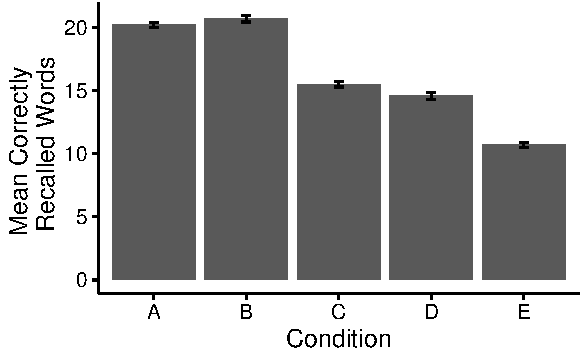
\includegraphics{Lab4_files/figure-latex/unnamed-chunk-5-1}

Now it is easy to the differences between conditions. Just as we had
hoped, Groups A and B appear to have recalled more words than Groups C
and D, which remembered more words than group E.

\subsection{Conducting the ANOVA}\label{conducting-the-anova}

Although the graph and the tabe show some clear differences in the
means, we still want to find out the probability that this kind of
finding occurs by chance alone. We can be confident in the differences
when we know that they do not occur very often by chance alone. The
first step is conduct a one-way ANOVA. This is very easy in R.

\begin{Shaded}
\begin{Highlighting}[]
\NormalTok{aov.out<-}\KeywordTok{aov}\NormalTok{(Recall~Conditions,long_data)}
\end{Highlighting}
\end{Shaded}

We're done! It's only one line of code. However, we need a couple more
to see the results.

\begin{Shaded}
\begin{Highlighting}[]
\NormalTok{aov_summary<-}\KeywordTok{summary}\NormalTok{(aov.out)}
\KeywordTok{kable}\NormalTok{(}\KeywordTok{xtable}\NormalTok{(aov_summary),}\DataTypeTok{format=}\StringTok{"latex"}\NormalTok{)}
\end{Highlighting}
\end{Shaded}

\begin{tabular}{l|r|r|r|r|r}
\hline
  & Df & Sum Sq & Mean Sq & F value & Pr(>F)\\
\hline
Conditions & 4 & 694.52 & 173.630000 & 32.46095 & 0\\
\hline
Residuals & 45 & 240.70 & 5.348889 & NA & NA\\
\hline
\end{tabular}

The ANOVA table gives us a bunch of information. We will go into much
greater detail about the meaning of each number in the table, but also
assume for now that you are somewhat familiar with these ideas because
you have already taken statistics, right?

We are mainly interested in the p-value, which tells how often results
like the ones we found can occur by chance. But, when we report the
results of our ANOVA, we also provide additional information about the
F-value, the degrees of freedom values, and the mean squared error term.
The reason is that if you know these numbers, you can actually
reconstruct all of the other numbers. The results of our ANOVA are
significant. You could report this in a sentence like the following.

The main effect of condition was significant, F(4, 45) = 32.46, MSE =
5.35, p \textless{} .001.

\subsection{Comparisons between
conditions}\label{comparisons-between-conditions}

The p-value from above is much smaller than .05, which shows the
difference between conditions in the data does not occur very often by
chance alone. However, because we conducted an omni-bus test, we only
know that there is some difference between conditions, but we do not
know which specific conditions are different from one another.

So, we have to conduct additional tests between specific conditions.
There are multiple strategies for conducting these tests. For now, we
will simply run t-tests between comparisons of interest.

Remember, our data simulated the pattern that memory recall would be
better for groups A and B, which would be better than groups C and D,
which would better than group E. In other words A=B \textgreater{} C=D
\textgreater{} E.

We can confirm this pattern by conducting tests to see if it holds up.
For example, how would we test the pattern A=B \textgreater{} C=D
\textgreater{} E, all of the following comparisons need to be true,

\begin{itemize}
\item
  A = B
\item
  A \textgreater{} C
\item
  A \textgreater{} D
\item
  B \textgreater{} C
\item
  B \textgreater{} D
\item
  C = D
\end{itemize}

and, all of the conditions should be greater than E

\begin{itemize}
\item
  A \textgreater{} E
\item
  B \textgreater{} E
\item
  C \textgreater{} E
\item
  D \textgreater{} E
\end{itemize}

Let's conduct a few of these tests, and then report the findings.

\begin{Shaded}
\begin{Highlighting}[]
\KeywordTok{library}\NormalTok{(broom)}
\CommentTok{#conduct t-tests}
\NormalTok{ab<-}\KeywordTok{tidy}\NormalTok{(}\KeywordTok{t.test}\NormalTok{(A,B,}\DataTypeTok{var.equal =} \OtherTok{TRUE}\NormalTok{))}
\NormalTok{ac<-}\KeywordTok{tidy}\NormalTok{(}\KeywordTok{t.test}\NormalTok{(A,C,}\DataTypeTok{var.equal =} \OtherTok{TRUE}\NormalTok{))}
\NormalTok{cd<-}\KeywordTok{tidy}\NormalTok{(}\KeywordTok{t.test}\NormalTok{(C,D,}\DataTypeTok{var.equal =} \OtherTok{TRUE}\NormalTok{))}
\NormalTok{de<-}\KeywordTok{tidy}\NormalTok{(}\KeywordTok{t.test}\NormalTok{(D,E,}\DataTypeTok{var.equal =} \OtherTok{TRUE}\NormalTok{))}

\CommentTok{#put the results in a table}
\NormalTok{alltests<-}\KeywordTok{rbind}\NormalTok{(ab,ac,cd,de)}
\NormalTok{alltests<-}\KeywordTok{cbind}\NormalTok{(alltests,}\DataTypeTok{Comparison=}\KeywordTok{c}\NormalTok{(}\StringTok{"AB"}\NormalTok{,}\StringTok{"AC"}\NormalTok{,}\StringTok{"CD"}\NormalTok{,}\StringTok{"DE"}\NormalTok{))}
\NormalTok{finaltable <-}\StringTok{ }\KeywordTok{subset}\NormalTok{(alltests, }\DataTypeTok{select =} \KeywordTok{c}\NormalTok{(Comparison,estimate1,estimate2,statistic,p.value,parameter))}
\KeywordTok{kable}\NormalTok{(finaltable,}\DataTypeTok{format=}\StringTok{"latex"}\NormalTok{)}
\end{Highlighting}
\end{Shaded}

\begin{tabular}{l|r|r|r|r|r}
\hline
Comparison & estimate1 & estimate2 & statistic & p.value & parameter\\
\hline
AB & 20.2 & 20.7 & -0.4900286 & 0.6300329 & 18\\
\hline
AC & 20.2 & 15.5 & 5.2511144 & 0.0000541 & 18\\
\hline
CD & 15.5 & 14.6 & 0.8181818 & 0.4239528 & 18\\
\hline
DE & 14.6 & 10.7 & 3.5851808 & 0.0021158 & 18\\
\hline
\end{tabular}

\subsection{Writing it all up}\label{writing-it-all-up}

The following is an example results section for our hypothetical
experiment. This could serve as a model for your own results section.

The number of correctly recalled words for each subject in each
condition were submitted to a one-way ANOVA, with memorization condition
(A, B, C, D, and E) as the sole between-subjects factor. Mean recall
scores in each condition are displayed in Figure 1.

The main effect of memorization condition was significant, F(4, 45) =
32.46, MSE = 5.35, p \textless{} .001. Figure 1 shows that Groups A and
B had higher recall scores than Groups C and D, which had higher recall
scores than Group E. This pattern was confirmed across four independent
sample t-tests. Group A (M = 20.2) and Group B (M = 20.7) were not
significantly different t(18) = -0.49, p =0.63. Group A recalled
significantly more words than Group C (M = 15.5), t(18) = 5.25, p =0.
Group C and Group D (M = 14.6) were not significantly different t(18) =
0.82, p =0.424. Finally, Group D recalled significantly more words than
Group E (M = 10.7), t(18) = 3.59, p =0.002.











\chapter{Lab 5: Task-Switching Mini Project}
\lhead{\allcaps{Lab 5: Task-Switching Mini Project}}
\openepigraph{The secret to multitasking is that it isn't actually multitasking. It's just extreme focus and organization.
}{---Joss Whedon}


In the second mini-project, you will read, summarize and discuss the paper by \citeauthor{stoet_are_2013} (2013)\cite{stoet_are_2013}. Then, you will attempt to replicate their results in the lab, by conducting an experiment and analyzing the data.

\section{What's in store}

\begin{enumerate}
\item Students read paper and write QALMRI (15-20)
\item Group discussion about paper (15-20)
\item Students download the task-switching program available from the website and individually complete the task. Individual students then enter their data in the master spreadsheet
\item Discussion of how to analyze the data. Major analysis goals are:

a.	Was there a mixing cost? Compare pure lists to mixed lists

b.	Was there a switching cost? Compare switch vs. repeat trials in pure lists

c.	Did these effects depend on gender? Did the women have a smaller mixing cost than the men? Did the women have a smaller switching cost than the men?

\item Students break into groups to analyze the data.

\end{enumerate}

\section{Critical Concepts}

\subsection{Multiple Dependent and Independent Variables}

In lab 5 we begin looking at more complex designs that involve multiple dependent or and independent variables. For example, we can look at the dependent variable of reaction time or error rate, which are our two difference measured variables. There are also three independent variables, including gender (male vs female), block (pure list vs. mixed list), and trial sequence (repeat trial vs. switch trial). 

\subsection{Main effects and interactions}
Throughout this course we will be talking a lot about main effects and interactions. Feel free to jump ahead in the textbook and learn more about them. 

Main effects refer to the influence of single independent variables. And, each independent variable always has one main effect. So, we could look at the main effect of gender, block, or trial sequence. The main effect is like conducting a one-way ANOVA on the variable of interest, collapsing over the other variables. For example, a main effect of trial sequence usually shows slower mean reaction times in the switch condition compared to the repeat condition. This is called the task-switching cost, or also the task-switching effect.

Interactions occur when the effect of one independent variable depends on the levels of another independent variable. For example, if women actually multi-task better than men, then we should expect an interaction between gender and task-switching. Specifically, women should be better at task-switching than men. This would mean that women should have smaller task-switching costs (meaning they are unaffected by switching) compared to men (who should have bigger task-switching costs if they are more affected by switching).

If women have smaller task switching costs than men, then the effect of task-switching independent variable (repeat vs. switch) will depend on the level of the gender variable (women vs. men), which is the definition of an interaction.

\subsection{Manipulating an Effect}

Things get complicated when we add more dependent and independent variables, and it can be easy to lose track of what is going on in an experiment.

Many experiments are conducted for the purpose of better understanding some phenomena. For example, researchers observe phenomena like the task-switching effect, they create theories to explain the phenomena, then they test their theories by running more experiments. 

A primary question is often to identify factors that manipulate, influence, or somehow change the phenomena of interest. We know that switching between tasks can hurt performance, and we measure this cost by calculating a switch cost, which is the difference in performance between switching conditions and repeating conditions. What kinds of factors would make this cost ? Perhaps extended practice, time of day, gender, personality, motivation, drug interventions, details of the task, and many other factors could make the normal cost get smaller. Many of these factors might also make the effect get larger. And, knowledge of what makes switching costs smaller or larger can be used to test theories, which need to explain how and why those factors cause switching costs to change. 

The Stoet et al. (2013) took this approach to determine if switch costs are smaller for men than women. Notice we have been talking about switch costs, which is the phenonemon and effect of interest. We have not been talking too much about the dependent variable of reaction times that we use to compute the switch costs. Remember that switch costs are computed as RT switch - RT repeat.

\subsection{Reducing a two-factor design to a single-factor design using difference scores}

We can use the term switch cost as a convenient term to describe the effect of the switching variable on reaction times. We can also think of the switch cost as the dependent variable of interest, rather than the base reaction time scores. Thinking of the switch cost this way can change how you conceptualize the design.

For example, how many independent variables are in a design testing whether women have smaller switch costs than men? The answer could be two or one, depending on how you think of the design.

If we go with two, then the design involves the independent variables gender (women vs. men) and trial sequence (switch vs. repeat), and the dependent variable of reaction time. This design would have two main effects (effect of gender, and effect of switching), and one interaction (gender x switching). We would be mainly interested in the interaction. For example, women may have a smaller difference in mean reaction time between the switch and repeat conditions than men. 

We can reduce the design to a simple single-factor design. To do so, we create a new dependent variable called switch costs. For example, for each subject we compute the mean reaction in the switch and repeat condition. Then we  calculate the switch costs (difference between switch and repeat) for each subject. Now, each subject has one switch cost, rather than two reaction times. Now, the design would have gender as the single independent variable, and switch costs as the dependent variable. To determine whether women have smaller costs than men would you could run a t-test comparing the switch-costs between conditions.




\section{Data-analysis tips}\label{lab-5-data-analysis-tips}

To give you an idea about the analyses you will be performing, we will
again create simulated data to mimic aspects of the experiment, and then
go through the steps of performing the analysis.

We will simulate data for the switching cost. Specifically, we will
imagine that women have a smaller switching cost than men. The code
below generates sample data for 10 women and 10 men, who each have mean
reactions in the repeat and switch conditions. For women, the mean
reaction times were 580 ms for repeat and 600 ms for switch sequences,
for a total expected switch cost of 20 ms. For men, the mean reaction
times were 580 ms for repeat and 650 ms for switch sequences, for a
total expected switch cost of 70 ms.

\subsection{Simulating the data}\label{simulating-the-data}

\begin{Shaded}
\begin{Highlighting}[]
\NormalTok{women_switch <-}\KeywordTok{round}\NormalTok{(}\KeywordTok{rnorm}\NormalTok{(}\DecValTok{10}\NormalTok{,}\DecValTok{600}\NormalTok{,}\DecValTok{20}\NormalTok{))}
\NormalTok{women_repeat <-}\KeywordTok{round}\NormalTok{(}\KeywordTok{rnorm}\NormalTok{(}\DecValTok{10}\NormalTok{,}\DecValTok{580}\NormalTok{,}\DecValTok{20}\NormalTok{))}
\NormalTok{men_switch <-}\KeywordTok{round}\NormalTok{(}\KeywordTok{rnorm}\NormalTok{(}\DecValTok{10}\NormalTok{,}\DecValTok{650}\NormalTok{,}\DecValTok{20}\NormalTok{))}
\NormalTok{men_repeat <-}\KeywordTok{round}\NormalTok{(}\KeywordTok{rnorm}\NormalTok{(}\DecValTok{10}\NormalTok{,}\DecValTok{580}\NormalTok{,}\DecValTok{20}\NormalTok{))}
\NormalTok{all_data<-}\KeywordTok{data.frame}\NormalTok{(}\DataTypeTok{Subject=}\KeywordTok{c}\NormalTok{(}\KeywordTok{rep}\NormalTok{(}\KeywordTok{seq}\NormalTok{(}\DecValTok{1}\NormalTok{,}\DecValTok{10}\NormalTok{,}\DecValTok{1}\NormalTok{),}\DecValTok{2}\NormalTok{),}
                               \KeywordTok{rep}\NormalTok{(}\KeywordTok{seq}\NormalTok{(}\DecValTok{11}\NormalTok{,}\DecValTok{20}\NormalTok{,}\DecValTok{1}\NormalTok{),}\DecValTok{2}\NormalTok{)),}
                     \DataTypeTok{Gender=}\KeywordTok{rep}\NormalTok{(}\KeywordTok{c}\NormalTok{(}\StringTok{"Female"}\NormalTok{,}\StringTok{"Male"}\NormalTok{),}\DataTypeTok{each=}\DecValTok{20}\NormalTok{),}
                     \DataTypeTok{Sequence=}\KeywordTok{rep}\NormalTok{(}\KeywordTok{rep}\NormalTok{(}\KeywordTok{c}\NormalTok{(}\StringTok{"switch"}\NormalTok{,}\StringTok{"repeat"}\NormalTok{),}\DataTypeTok{each=}\DecValTok{10}\NormalTok{),}\DecValTok{2}\NormalTok{),}
                     \DataTypeTok{RT=}\KeywordTok{c}\NormalTok{(women_switch,women_repeat,}
                          \NormalTok{men_switch,men_repeat))}

\KeywordTok{kable}\NormalTok{(all_data,}\DataTypeTok{format=}\StringTok{"latex"}\NormalTok{)}
\end{Highlighting}
\end{Shaded}

\begin{tabular}{r|l|l|r}
\hline
Subject & Gender & Sequence & RT\\
\hline
1 & Female & switch & 572\\
\hline
2 & Female & switch & 621\\
\hline
3 & Female & switch & 569\\
\hline
4 & Female & switch & 609\\
\hline
5 & Female & switch & 574\\
\hline
6 & Female & switch & 598\\
\hline
7 & Female & switch & 590\\
\hline
8 & Female & switch & 623\\
\hline
9 & Female & switch & 586\\
\hline
10 & Female & switch & 590\\
\hline
1 & Female & repeat & 556\\
\hline
2 & Female & repeat & 566\\
\hline
3 & Female & repeat & 588\\
\hline
4 & Female & repeat & 611\\
\hline
5 & Female & repeat & 575\\
\hline
6 & Female & repeat & 582\\
\hline
7 & Female & repeat & 576\\
\hline
8 & Female & repeat & 578\\
\hline
9 & Female & repeat & 558\\
\hline
10 & Female & repeat & 581\\
\hline
11 & Male & switch & 660\\
\hline
12 & Male & switch & 657\\
\hline
13 & Male & switch & 622\\
\hline
14 & Male & switch & 651\\
\hline
15 & Male & switch & 664\\
\hline
16 & Male & switch & 623\\
\hline
17 & Male & switch & 642\\
\hline
18 & Male & switch & 676\\
\hline
19 & Male & switch & 659\\
\hline
20 & Male & switch & 618\\
\hline
11 & Male & repeat & 585\\
\hline
12 & Male & repeat & 571\\
\hline
13 & Male & repeat & 575\\
\hline
14 & Male & repeat & 594\\
\hline
15 & Male & repeat & 572\\
\hline
16 & Male & repeat & 605\\
\hline
17 & Male & repeat & 556\\
\hline
18 & Male & repeat & 650\\
\hline
19 & Male & repeat & 594\\
\hline
20 & Male & repeat & 606\\
\hline
\end{tabular}

\subsection{plotting the data}\label{plotting-the-data}

We can plot the data at least two ways. See the bar and line graphs
below. Note that the x-axis changes between graphs.

\begin{Shaded}
\begin{Highlighting}[]
\KeywordTok{library}\NormalTok{(ggplot2)}
\KeywordTok{library}\NormalTok{(plyr)}
\NormalTok{sde<-function(x)\{}\KeywordTok{sd}\NormalTok{(x)/}\KeywordTok{length}\NormalTok{(x)\}}
\NormalTok{plot_means<-}\KeywordTok{ddply}\NormalTok{(all_data,.(Gender,Sequence),summarise,}
                       \DataTypeTok{MeanRT=}\KeywordTok{mean}\NormalTok{(RT),}
                       \DataTypeTok{SE=}\KeywordTok{sde}\NormalTok{(RT))}

\NormalTok{limits <-}\StringTok{ }\KeywordTok{aes}\NormalTok{(}\DataTypeTok{ymax =} \NormalTok{MeanRT +}\StringTok{ }\NormalTok{SE, }\DataTypeTok{ymin =} \NormalTok{MeanRT -}\StringTok{ }\NormalTok{SE)}

\KeywordTok{ggplot}\NormalTok{(plot_means,}\KeywordTok{aes}\NormalTok{(}\DataTypeTok{x=}\NormalTok{Gender, }\DataTypeTok{y=}\NormalTok{MeanRT, }\DataTypeTok{group=}\NormalTok{Sequence,}\DataTypeTok{fill=}\NormalTok{Sequence))+}
\StringTok{  }\KeywordTok{geom_bar}\NormalTok{(}\DataTypeTok{position=}\StringTok{"dodge"}\NormalTok{,}\DataTypeTok{stat=}\StringTok{"identity"}\NormalTok{)+}
\StringTok{  }\KeywordTok{geom_errorbar}\NormalTok{(limits, }\DataTypeTok{width=}\NormalTok{.}\DecValTok{3}\NormalTok{,}\DataTypeTok{position=}\KeywordTok{position_dodge}\NormalTok{(.}\DecValTok{9}\NormalTok{))+}
\StringTok{  }\KeywordTok{theme_classic}\NormalTok{(}\DataTypeTok{base_size=}\DecValTok{12}\NormalTok{)+}
\StringTok{  }\KeywordTok{ylab}\NormalTok{(}\StringTok{"Mean RT"}\NormalTok{)+}
\StringTok{  }\KeywordTok{xlab}\NormalTok{(}\StringTok{"Trial sequence"}\NormalTok{)}
\end{Highlighting}
\end{Shaded}

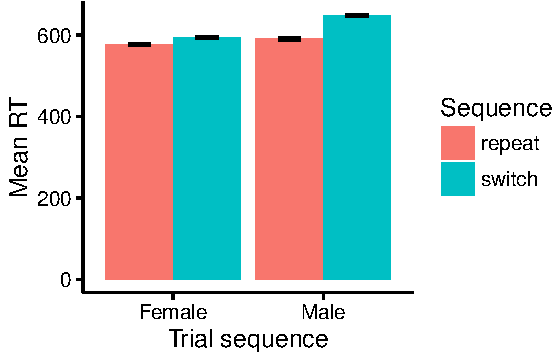
\includegraphics{Lab5_files/figure-latex/unnamed-chunk-2-1}

\begin{Shaded}
\begin{Highlighting}[]
\KeywordTok{ggplot}\NormalTok{(plot_means,}\KeywordTok{aes}\NormalTok{(}\DataTypeTok{x=}\NormalTok{Sequence, }\DataTypeTok{y=}\NormalTok{MeanRT, }\DataTypeTok{group=}\NormalTok{Gender,}\DataTypeTok{shape=}\NormalTok{Gender))+}
\StringTok{  }\KeywordTok{geom_line}\NormalTok{()+}
\StringTok{  }\KeywordTok{geom_point}\NormalTok{()+}
\StringTok{  }\KeywordTok{geom_errorbar}\NormalTok{(limits, }\DataTypeTok{width=}\NormalTok{.}\DecValTok{3}\NormalTok{)+}
\StringTok{  }\KeywordTok{theme_classic}\NormalTok{(}\DataTypeTok{base_size=}\DecValTok{12}\NormalTok{)+}
\StringTok{  }\KeywordTok{ylab}\NormalTok{(}\StringTok{"Mean RT"}\NormalTok{)+}
\StringTok{  }\KeywordTok{xlab}\NormalTok{(}\StringTok{"Trial sequence"}\NormalTok{)}
\end{Highlighting}
\end{Shaded}

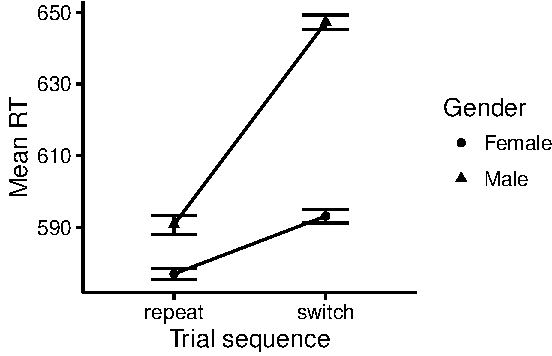
\includegraphics{Lab5_files/figure-latex/unnamed-chunk-3-1}

The graphs show that the switch costs (difference between repeat and
switch trials) is smaller for women and men. Which is good, because we
are simulating the data with this outcome in mind.

\subsection{Running the ANOVA}\label{running-the-anova}

The next step is to conduct an ANOVA. This design has two factors or
independent variables, gender and trial sequence. The gender variable is
between-subjects, and the trial sequence variable is within subjects.
So, we will run a 2 (Gender: Female vs.~Male) x 2 (trial sequence:
Repeat vs.~Switch) mixed design ANOVA with Gender as the betwen-subjects
factor, and trial sequence as the within-subjects factor.

\begin{Shaded}
\begin{Highlighting}[]
\KeywordTok{library}\NormalTok{(broom)}
\NormalTok{all_data$Subject<-}\KeywordTok{as.factor}\NormalTok{(all_data$Subject)}
\NormalTok{aov.out<-}\KeywordTok{aov}\NormalTok{(RT~Gender*Sequence+}\KeywordTok{Error}\NormalTok{(Subject/Sequence),all_data)}
\NormalTok{aov_summary<-}\KeywordTok{summary}\NormalTok{(aov.out)}
\KeywordTok{kable}\NormalTok{(}\KeywordTok{xtable}\NormalTok{(aov_summary),}\DataTypeTok{format=}\StringTok{"latex"}\NormalTok{)}
\end{Highlighting}
\end{Shaded}

\begin{tabular}{l|r|r|r|r|r}
\hline
  & Df & Sum Sq & Mean Sq & F value & Pr(>F)\\
\hline
Gender & 1 & 11458.225 & 11458.2250 & 22.10104 & 1.78e-04\\
\hline
Residuals & 18 & 9332.050 & 518.4472 & NA & NA\\
\hline
Sequence & 1 & 13140.625 & 13140.6250 & 38.47507 & 7.50e-06\\
\hline
Gender:Sequence & 1 & 4060.225 & 4060.2250 & 11.88813 & 2.87e-03\\
\hline
Residuals & 18 & 6147.650 & 341.5361 & NA & NA\\
\hline
\end{tabular}

\begin{Shaded}
\begin{Highlighting}[]
\NormalTok{mt<-}\KeywordTok{model.tables}\NormalTok{(aov.out,}\StringTok{"means"}\NormalTok{)}
\NormalTok{mt}
\end{Highlighting}
\end{Shaded}

\begin{verbatim}
## Tables of means
## Grand mean
##         
## 602.075 
## 
##  Gender 
## Gender
## Female   Male 
##  585.1  619.0 
## 
##  Sequence 
## Sequence
## repeat switch 
##  583.9  620.2 
## 
##  Gender:Sequence 
##         Sequence
## Gender   repeat switch
##   Female 577.1  593.2 
##   Male   590.8  647.2
\end{verbatim}

The above shows the ANOVA table and the means for the main effects and
interaction. We also conduct t.test comparisons to look at the switch
costs separately for men and women.

\begin{Shaded}
\begin{Highlighting}[]
\NormalTok{FemaleT<-}\KeywordTok{t.test}\NormalTok{(RT~Sequence,all_data[all_data$Gender==}\StringTok{"Female"}\NormalTok{,],}\DataTypeTok{paired=}\OtherTok{TRUE}\NormalTok{,}\DataTypeTok{var.equal=}\OtherTok{TRUE}\NormalTok{)}
\NormalTok{MaleT<-}\KeywordTok{t.test}\NormalTok{(RT~Sequence,all_data[all_data$Gender==}\StringTok{"Male"}\NormalTok{,],}\DataTypeTok{paired=}\OtherTok{TRUE}\NormalTok{,}\DataTypeTok{var.equal=}\OtherTok{TRUE}\NormalTok{)}
\NormalTok{FemaleT}
\end{Highlighting}
\end{Shaded}

\begin{verbatim}
## 
##  Paired t-test
## 
## data:  RT by Sequence
## t = -2.3034, df = 9, p-value = 0.04674
## alternative hypothesis: true difference in means is not equal to 0
## 95 percent confidence interval:
##  -31.9115634  -0.2884366
## sample estimates:
## mean of the differences 
##                   -16.1
\end{verbatim}

\begin{Shaded}
\begin{Highlighting}[]
\NormalTok{MaleT}
\end{Highlighting}
\end{Shaded}

\begin{verbatim}
## 
##  Paired t-test
## 
## data:  RT by Sequence
## t = -6.0205, df = 9, p-value =
## 0.0001975
## alternative hypothesis: true difference in means is not equal to 0
## 95 percent confidence interval:
##  -77.59196 -35.20804
## sample estimates:
## mean of the differences 
##                   -56.4
\end{verbatim}

\subsection{Writing up the results}\label{writing-up-the-results}

The next step is to interpret the results and write them up. Here is an
example write-up.

The mean reaction times for each subject in trial sequence condition
were submitted to a 2 (Gender: Female vs.~Male) x 2 (trial sequence:
Repeat vs.~Switch) mixed design ANOVA with Gender as the betwen-subjects
factor, and trial sequence as the within-subjects factor. Mean reaction
times in each condition collapsed across subjects are displayed in
Figure 1.

The main effect of gender was significant, F(1, 18) = 22.1, MSE =
518.45, p \textless{} 0. Women (585 ms) had faster mean reaction times
than men (619 ms).

The main effect of trials sequence was significant, F(1, 18) = 38.48,
MSE = 341.54, p \textless{} 0. Repeat trials (584) had faster mean
reaction times than switch trials (620).

Most important was the significant two-way interaction between gender
and trial sequence, F(1, 18) = 11.89, MSE = 341.54, p \textless{} 0.003.
We interpreted the interaction further by conducting the following
comparisons. Women showed a significant switch cost, t(9) = -2.3, p =
0.047, with faster mean reaction times for repeat (577) than switch
(593) trials. Men also showed a significant switch cost, t(9) = -6.02, p
= 0, with faster mean reaction times for repeat (591) than switch trials
(647). The presence of an interaction indicates that the size of the
switch cost for women was significantly smaller than the size of the
switch cost for men.










\chapter{Lab 6: Stroop Mini Project}
\lhead{\allcaps{Lab 6: Stroop Mini Project}}
\openepigraph{The simple act of paying attention can take you a long way.
}{---Keanu Reeves}


In the second mini-project, you will read, summarize and discuss the paper by \citeauthor{raz_suggestion_2006} (2013)\cite{raz_suggestion_2006}. This paper provides some background about the Stroop effect, which is a classic measure of selective attention, and then shows one manipulation that effectively helps people overcome Stroop interference. Your task in this lab will be to replicate the Stroop effect in one condition, and then attempt to change the size of the effect (make larger or smaller) in another condition.

\section{What's in store}

\begin{enumerate}
\item Students read paper and write QALMRI (15-20)
\item	Group discussion about paper (15-20)
\item	Students instructed their task is create their own Stroop design and employ a manipulation that increases or decreases the size of the Stroop effect
\item	Students break into groups and conduct a Stroop experiment, measuring the size of the Stroop effect in a "normal" condition, and in their manipulated condition.
\item	Groups analyze conduct a 2x2 ANOVA to see if their interaction was significant
\end{enumerate}

\section{Some background on the Stroop effect}

The Stroop effect is a well-known and classic phenomena in experimental psychology. The effect was first reported by J. R. Stroop (1935). Several hundreds of Stroop experiments have been conducted since 1935 and these experiments are summarized in Macleod's (1992) review.\cite{Stroop1935,macleod_half_1991}

The original Stroop task involved color naming of word stimuli that are printed in different ink colors. There are two important conditions involving congruent and incongruent item types. \emph{Congruent} items occur when the ink-color of the word matches the name of the word (e.g., the word red printed in red ink: \textcolor{red}{RED}). Incongruent items occur when the ink-color of the word does not match the name of the word (e.g., the word blue printed in red ink: \textcolor{red}{BLUE}). For each of these stimuli the task is to identify the ink-color of the word and ignore the written meaning of the word. Here are a few more examples of congruent and incongruent Stroop items:

Congruent: 	\textcolor{blue}{BLUE}, \textcolor{green}{GREEN}, \textcolor{yellow}{YELLOW}, \textcolor{red}{RED}

Incongruent:	\textcolor{red}{BLUE}, \textcolor{blue}{GREEN}, \textcolor{red}{YELLOW}, \textcolor{green}{RED} 

In the original set of experiments participants were presented with long lists of items and asked to read through the lists naming only the ink-colors and ignoring the word information. The important finding was that people were faster to finish reading lists that were composed of congruent items than incongruent items. This difference in reading time is termed the Stroop effect. For example, let’s say you were given a list of 60 congruent words and you read all of the ink-color names in 71 seconds. Next, you receive a list of 60 incongruent words and it takes you 94 seconds to read all of the ink-color names. You would compute your Stroop effect by taking the difference between the Congruent and Incongruent reading times. Congruent reading times are subtracted from incongruent reading times to give a positive Stroop effect value:

Stroop effect = Incongruent – Congruent  = 94 seconds – 71 seconds =  23 seconds

The Stroop test can be administered in many different ways. A common modern variant of the task is to present a single Stroop item on a computer screen per trial and have participants identify the ink-color by pressing a key or typing out the response. Several trials could be presented over the course of an experimental session, and the experimenter could vary whether upcoming trials are congruent or incongruent. The trial-based version of the Stroop procedure provides more experimental control and more precise measurement of reaction times.  This provides a more fine-grained measure of the time taken to respond congruent and incongruent items. Stroop effects using this procedure are usually measured in the milliseconds (ms). For example, reaction times for congruent items are usually around 500 ms, and reaction times for incongruent items are usually around 600 ms. So, the overall Stroop effect might be around 100 ms. 

\subsection{Stroop and Selective Attention}

The Stroop effect has been used as a tool to study various aspects of learning and attention. For example the Stroop effect has been used as a tool to study cognitive control. Cognitive control refers broadly to the psychological processes that allow people to plan, coordinate, and execute actions necessary to accomplish goals. A central aspect of cognitive control involves the attention processes that are responsible for selecting task-relevant information and ignoring task-irrelevant information when performing a task. 

The Stroop procedure provides a simple, yet effective, method for presenting people with two sources of information, one that is task-relevant (color) and one that is task-irrelevant (word). For this reason, Stroop items are sometimes referred to as bi-valent stimuli, in that they present two sources of information. Congruent Stroop items (blue in blue) do not present much of a selective attention challenge, both the word and the color information point to the same response. Incongruent items (blue in red) do present a selective attention challenge, the color points to the correct response and the word points to an incorrect response. When faced with incongruent items people must pay attention to the relevant color information and ignore or somehow filter out the irrelevant word information. The fact that people get Strooped, or that the Stroop effect exists at all, tells us something important about selective attention in this task. Specifically, people can not completely ignore the irrelevant word information. If people could completely ignore the irrelevant word information then the Stroop effect would cease to appear. People would be just as fast identifying congruent and incongruent items because they would be able to successfully ignore word information. 

Using the logic above the Stroop effect is often taken as a measure of selective attention ability. This means that changes in the size of the Stroop effect may represent differences in selective attention ability. People who have very large Stroop effects have poor attentional control over their ability to ignore the word stimulus. People who have very small Stroop effects have excellent attentional control over their ability to ignore the word stimulus. 






\chapter{Labs 7 and 8: Paper Project 2 }
\lhead{\allcaps{Labs 7 and 8: Paper Project 2}}
\openepigraph{The purpose of psychology is to give us a completely different idea of the things we know best.}{---Paul Valery}


\section{Overview}

In this project you will attempt to replicate a classic study on face perception (Yin, 1969)\cite{yin_looking_1969}. A replication of the experiment has already been designed. To collect data, you will first participate as a subject in the experiment. Then, as a class you will be introduced to the published paper. You will read the paper and it in class. Then, the class will analyze the collected data to determine whether or not the major effects of interest have been replicated. Data will be collected using pen and paper methods, and analyzed by computer software. Each student will write a 5+ page, APA style report on the project.

\subsection{Things you will learn:}

\begin{itemize}
\item Reading and citing primary source material
\item Writing a brief APA style research report
\item Conducting and reporting Factorial designs
\end{itemize}

\subsection{Background readings:}

Available on the lab website, or download from Brooklyn College library 

\subsection{Grade}
\begin{itemize}
\item  10\% of final grade
\item Graded by your lab instructor. Lab instructor sets due date, and determines whether revised drafts are submittable.
\item If you submit completed versions of all paper assignments (1, 2, and 3), then you get to drop your lowest paper grade from paper 1 or 2. Specifically, you will receive your highest grade from paper 1 or 2 for both papers, thereby eliminating the lower grade. This allows room to learn and improve as you go. 
\end{itemize}


\section{Writing the paper}

There are many resources for help on writing an APA style research report in the lab manual, on the textbook, and the website. Check them out. As well, here is a rough roadmap for writing paper 2.

\subsection{APA formatting, Title and Abstract}

\begin{itemize}
\item Use APA formatting rules.

\item Create a suitable title for the paper

\item Write the abstract : No more than 250 words. The aim is to briefly describe the issue at hand, the experiment, and the results.
\end{itemize}

\subsection{Introduction (around 2 double-spaced pages)}

The goal of the introduction is to first put the research into a broader context, and then narrow the focus to describe the specific research aims.

\begin{enumerate}
\item A. Opening section: (starting broad)

\begin{itemize}
\item about 1 paragraph
\item Discuss a real-world example of the general phenomena under investigation by the paper
\item Tell the reader that the purpose of the current experiment is to conduct a replication of the work in question
\item  Establish the domain and big questions.
\end{itemize}

\item Middle section: Prior work

\begin{itemize}
\item Discuss some examples of previous research that are similar to the present research. You have an opportunity here to look this kind of research up on Google Scholar. One or two examples ought to be enough.
\item Explain the specific question that is being asked in this replication work.
\end{itemize}

\item Final section: (briefly explain the present aims, the experiment and what you expect to find)
\begin{itemize}
\item Explain the hypotheses (alternatives)
\item Explain the logic of how the hypotheses will be tested
\item Briefly explain what the participants will be doing in the task
\item Briefly give predictions for performance in each condition
\end{itemize}

\end{enumerate}


\subsection{Methods (about 1 page)}

The methods section should be a complete recipe that anyone could follow to replicate your experiment. There are lots of details that you can include, some of these are listed below. Be brief and concise

\begin{enumerate}
\item Participants
	\begin{itemize}
	\item how many people?
	\item where did they come from?
	\end{itemize}
\item Materials
	\begin{itemize}
	\item what were the stimuli?
	\item how were they organized?
	\end{itemize}

\item Design \& Procedure
	\begin{itemize}
	\item What was the design
	\item What were the independent variable(s)
	\item What was the dependent variable
	\item Within or between subjects?
	\item How were the stimuli for each trial chosen
	\item Describe the steps each participant took to complete the experiment
	\end{itemize}

\end{enumerate}

\subsection{Results}

The result section is used to report the patterns in the data, and the statistical support for those patterns. You will compute the results using SPSS in the lab computers. The lab manual can be consulted for help on running statistical tests, and for reporting results.

\begin{itemize}
\item Describe the statistical analysis
\item Tell the reader where they can see the data. E.g., the results of experiment 1 are presented in table 1, or in figure 1
\item Make a table or figure to display the data in your paper
\item Report the statistical test, and the pattern of the means.
\end{itemize}

\subsection{Discussion}

The discussion can be used to briefly restate verbally the pattern of the most important results, and then to relate the results to theory and ideas developed in the introduction

\begin{itemize}
\item Highlight the main findings from the experiment
\item Discuss how the data can be explained by the hypothesis. What inferences do you make about the hypotheses based on the research findings?
\item Broaden your discussion. Can the findings be explained by an alternative theory? What can be generalized to the real world? Are there important confounds that prevent us from interpreting our results?
\end{itemize}

\subsection{References and Figures or Tables}

\begin{itemize}
\item Include citations used in the paper using APA style format
\item Include a figure or table to show the results
\end{itemize}

%
\section{Data-analysis tips}\label{lab-1-data-analysis-tips}

In lab one you will be collecting measurements on several dependent
variables, in each of two manipulated conditions (the independent
variable). For each dependent variable you will want to determine
whether the manipulation had an effect. That is, did the independent
variable cause a change in the dependent variable. We know that
differences can sometimes be observed by chance alone, so we want to
conduct an inferential statistical test to determine the probability
that our observed difference could have been produced by chance alone.
To do this we will be conducting several t-tests. This is a short primer
on the process. You can conduct t-tests in the software of your choice,
or by hand using a calculator (or in excel). Here, we will use the free
and open-source statistical package called R, to illustrate the process.

Let's imagine we have two groups of 10 subjects each. Group A receives
condition 1 of the independent variable, and Group B recieves condition
2 of the independent variable. We then measure some behavior for all of
the subject in all of the groups. To make this more concrete, let's say
10 subjects drink coffee, and the the 10 subjects drink tea. Then we
present all of the subjects with a piece of art and ask them rate how
beautiful they think it is on a scale from 1 to 7.

When we collect all the data we should have 20 total ratings, one for
each subject in each group.

For example, if you put the data in a table it might look something like
the following. Note, the grey text box shows the R code used to simulate
the data. For, each group, we sample 10 numbers from a normal
distribution with a mean of 4, and a standard deviation of .5. Then we
put the numbers in a table.

\begin{Shaded}
\begin{Highlighting}[]
\NormalTok{coffee<-}\KeywordTok{round}\NormalTok{(}\KeywordTok{rnorm}\NormalTok{(}\DecValTok{10}\NormalTok{,}\DecValTok{4}\NormalTok{,.}\DecValTok{5}\NormalTok{))}
\NormalTok{tea<-}\KeywordTok{round}\NormalTok{(}\KeywordTok{rnorm}\NormalTok{(}\DecValTok{10}\NormalTok{,}\DecValTok{4}\NormalTok{,.}\DecValTok{5}\NormalTok{))}
\NormalTok{all_data<-}\KeywordTok{data.frame}\NormalTok{(coffee,tea)}
\KeywordTok{kable}\NormalTok{(all_data,}\DataTypeTok{format=}\StringTok{"latex"}\NormalTok{)}
\end{Highlighting}
\end{Shaded}

\begin{tabular}{r|r}
\hline
coffee & tea\\
\hline
4 & 5\\
\hline
3 & 4\\
\hline
3 & 4\\
\hline
3 & 3\\
\hline
4 & 3\\
\hline
4 & 5\\
\hline
4 & 4\\
\hline
4 & 4\\
\hline
4 & 4\\
\hline
3 & 4\\
\hline
\end{tabular}

We can do some quick descriptive statistics, for example, we might want
to know the means of the beauty ratings for the coffee and tea groups.

\begin{Shaded}
\begin{Highlighting}[]
\KeywordTok{mean}\NormalTok{(coffee)}
\end{Highlighting}
\end{Shaded}

\begin{verbatim}
## [1] 3.6
\end{verbatim}

\begin{Shaded}
\begin{Highlighting}[]
\KeywordTok{mean}\NormalTok{(tea)}
\end{Highlighting}
\end{Shaded}

\begin{verbatim}
## [1] 4
\end{verbatim}

The means aren't very different, and of course we should expect they
should be similar. After all, we sampled these means from the exact same
distribution. So, we should expect that on average, the means should
both be close to 4. However, they won't necessarilly be exactly 4,
because of variability introduced by random sampling.

\section{The t-test}\label{the-t-test}

What we want to do next is conduct an independent samples t-test. We
want to determine whether any possible difference between the coffee and
tea groups could have been produced by chance alone. We can conduct a
t-test in R very easily using the t.test function.

\begin{Shaded}
\begin{Highlighting}[]
\KeywordTok{t.test}\NormalTok{(coffee,tea,}\DataTypeTok{var.equal=}\OtherTok{TRUE}\NormalTok{)}
\end{Highlighting}
\end{Shaded}

\begin{verbatim}
## 
##  Two Sample t-test
## 
## data:  coffee and tea
## t = -1.5, df = 18, p-value = 0.151
## alternative hypothesis: true difference in means is not equal to 0
## 95 percent confidence interval:
##  -0.9602459  0.1602459
## sample estimates:
## mean of x mean of y 
##       3.6       4.0
\end{verbatim}

R gives us back the t values, the degrees of freedom (df), and the
associated p-value. The p-value tells us the likelihood that our
difference, or a difference greater than the one we observed could have
been produced by chance.

\section{One more time}\label{one-more-time}

Let's try this whole process again, but this time we will simulate data
with an actual difference between the groups. For example, let's say we
want to simulate the idea that drinking coffee makes people think the
art is less beautiful by at least 2 points, and then reconduct the
t-test with the new simulated data. We will sample numbers from a normal
distribution with mean 3 for the coffee group, and mean 5 for the tea
group (for an average expected difference of 2).

\begin{Shaded}
\begin{Highlighting}[]
\NormalTok{coffee<-}\KeywordTok{round}\NormalTok{(}\KeywordTok{rnorm}\NormalTok{(}\DecValTok{10}\NormalTok{,}\DecValTok{3}\NormalTok{,.}\DecValTok{5}\NormalTok{))}
\NormalTok{tea<-}\KeywordTok{round}\NormalTok{(}\KeywordTok{rnorm}\NormalTok{(}\DecValTok{10}\NormalTok{,}\DecValTok{5}\NormalTok{,.}\DecValTok{5}\NormalTok{))}
\NormalTok{all_data<-}\KeywordTok{data.frame}\NormalTok{(coffee,tea)}
\KeywordTok{kable}\NormalTok{(all_data,}\DataTypeTok{format=}\StringTok{"latex"}\NormalTok{)}
\end{Highlighting}
\end{Shaded}

\begin{tabular}{r|r}
\hline
coffee & tea\\
\hline
3 & 5\\
\hline
3 & 5\\
\hline
3 & 4\\
\hline
3 & 6\\
\hline
2 & 5\\
\hline
4 & 5\\
\hline
3 & 6\\
\hline
3 & 5\\
\hline
3 & 5\\
\hline
3 & 5\\
\hline
\end{tabular}

\begin{Shaded}
\begin{Highlighting}[]
\KeywordTok{mean}\NormalTok{(coffee)}
\end{Highlighting}
\end{Shaded}

\begin{verbatim}
## [1] 3
\end{verbatim}

\begin{Shaded}
\begin{Highlighting}[]
\KeywordTok{mean}\NormalTok{(tea)}
\end{Highlighting}
\end{Shaded}

\begin{verbatim}
## [1] 5.1
\end{verbatim}

\begin{Shaded}
\begin{Highlighting}[]
\KeywordTok{t.test}\NormalTok{(coffee,tea,}\DataTypeTok{var.equal=}\OtherTok{TRUE}\NormalTok{)}
\end{Highlighting}
\end{Shaded}

\begin{verbatim}
## 
##  Two Sample t-test
## 
## data:  coffee and tea
## t = -9, df = 18, p-value = 4.404e-08
## alternative hypothesis: true difference in means is not equal to 0
## 95 percent confidence interval:
##  -2.590215 -1.609785
## sample estimates:
## mean of x mean of y 
##       3.0       5.1
\end{verbatim}

\section{Writing up the results of a
t-test}\label{writing-up-the-results-of-a-t-test}

We've now conducted two different t-tests, and received different
results on each them. You will likely find different results for all of
the t-tests that you conduct for the lab experiment. However, you will
use the basic sentence structure to report all of the results. When you
report the results of your experiment along with statistical tests there
are two important features to include, the pattern of the results, and
the inferential statistic. In this situation, we would simply report the
means and the t-test information. Here are is an with made-up numbers.

The coffee group gave a lower mean beauty rating (M = 3.4) than the tea
group (M = 5.6), and the difference was significant, t (18) = 5.4, p
\textless{} .001.

So, just in one sentence we tell the reader what the means were in both
conditions, as whether the result was significant. APA style recommends
reporting exact p-values when they are greater than .001 (for example p
= .047). If the p-value is less than .001, then you just need to report
p \textless{} .001.







\chapter{Labs 9 - 14: The Final Project}
\lhead{\allcaps{Labs 9 - 14: The Final Project}}
\openepigraph{The purpose of psychology is to give us a completely different idea of the things we know best.}{---Paul Valery}

\section{Overview}

Your task for the final project is to design and run your own experiment. There are 3 major components.

\begin{itemize}
\item 2-3 minute individual presentation
\item Individual APA research report
\item 10 minute group presentation
\end{itemize}

For your individual presentation you will have the opportunity to develop your own experimental idea. Following the individual presentations you will be divided into smaller groups, and will decide on a final experiment idea. Each group will be required to have their experimental design approved by the lab instructor. Once the experiment is approved data collection can begin. Your lab instructors will help you with your experimental design to ensure that your project is feasible given the constraints that you are working with. Every student in the group will be responsible for writing their own APA research report on the findings of the experiment conducted by the group. As well as the paper, each group will be responsible for a 10 minute presentation that explains the findings of the research.

\subsection{Requirements}

The following applies for all aspects of the following assignments.

\begin{enumerate}
\item The final project (or proposal for individual presentation) must be a factorial design with two manipulated independent variables.
\item The project must identify an effect from the literature that can be measured by one of the independent variables. For example, the choice of effect could be the Stroop effect, in which case the first independent variable would be congruency (congruent vs. incongruent).
\item The second independent variable will involve a manipulation intended to influence the size of the effect under investigation. The manipulation could be intended to increase the size of the effect relative to an established condition, or to decrease or eliminate the the effect. For example, in a Stroop experiment, the second independent variable could be word-size, and the empirical question could be whether the Stroop effect is larger when the words are printed in a large font, compared to when the words are printed in a smaller font.
\item In other words, the design of the final project will attempt to produce an interaction effect.
\end{enumerate}

\subsection{2-3 minute individual presentation (5\% of total grade)}

Every student is responsible for one 2-3 minute presentation that outlines their proposal for the final project. After the presentation, students will form groups, and the groups will decide on a particular proposal for the final project (from the presentations, or a new proposal)

Each individual presentation at a minimum should accomplish the following:
\begin{itemize}
\item Describe the effect that will be studied
\item Describe the proposed manipulation that will influence the effect
\item Show the predicted results in a graph
\item Explain the hypothesis or theory that would lead you to predict those results
\end{itemize}

Presentations should be made in powerpoint. You are allowed to develop any kind of experiment that interests you. However, your experiment must involve a factorial design. 

\subsection{APA style research report (15\% of total grade)}

Every student will be responsible for reporting the findings of their group experiment in an APA style research report. The paper should have a minimum of 5 pages, and should include an introduction, methods section, results section, discussion, and reference section. The paper should contain at least 3 citations to relevant papers from the psychological literature. The format of the paper will be identical to all of the previous labs. The paper is not a group assignment. Each student will write their own paper.

\subsection{10 minute group presentation (5\% of total grade)}

After data collection and data analysis has taken place, each group will be responsible for presenting their findings. The group presentation should last approximately 10 minutes. The group presentation should be shared amongst the members of the group, with each member responsible for presenting a section of the material. The following material should be covered in the presentation:

\begin{itemize}
\item Explain relevant background knowledge
\item Explain the hypothesis under investigation
\item Explain the proposed design of the experiment
\item Explain the predicted findings of the experiment
\item Explain the actual findings
\item Discuss the meaning of the findings as they relate to the hypotheses under investigation.
\end{itemize}

\chapter{Statistical Analysis And Reporting}
\lhead{\allcaps{Statistical Analysis And Reporting}}
\openepigraph{Memory... is the diary that we all carry about with us.}{---Oscar Wilde}

\section{Excel Tips}

This document gives a brief introduction to using excel for data analysis. The guide covers basic excel operation, formula use, and pivot tables. Many first time users will find aspects of excel confusing, this guide is intended to give you enough basic knowledge to get you started. There are extensive help guides published on the internet, and if you find yourself confronted with a problem that is not discussed here you will often find valuable help by searching Google for the answer. If you have suggestions for excel tips that should be included in this document please let your lab instructor know.

\subsection{What is Excel?}

Excel is a spreadsheet tool. It allows you to organize and analyze data that are stored in column and row format. Excel is extremely powerful. With enough know-how almost all of the data analysis that statistics programs like SPSS are built for, can be accomplished directly in Excel. 


\subsection{What is Excel used for in this course?}


You can use excel (or another spreadsheet program) to:


\begin{itemize} 

\item Store your data, 

\item to perform basic analysis of your data (e.g., getting averages and standard deviations, computing correlations etc.), and 

\item to create figures, graphs, and tables to present your data.
\end{itemize}


\section{Using Excel}

\subsection{The excel window}
 
Excel is a spreadsheet that contains different rows (the numbers), and different columns (the letters).
The individual cells can be used to hold data in the form of numbers or letters, to analyze data, and to report data using tables and figures.

\begin{figure}
      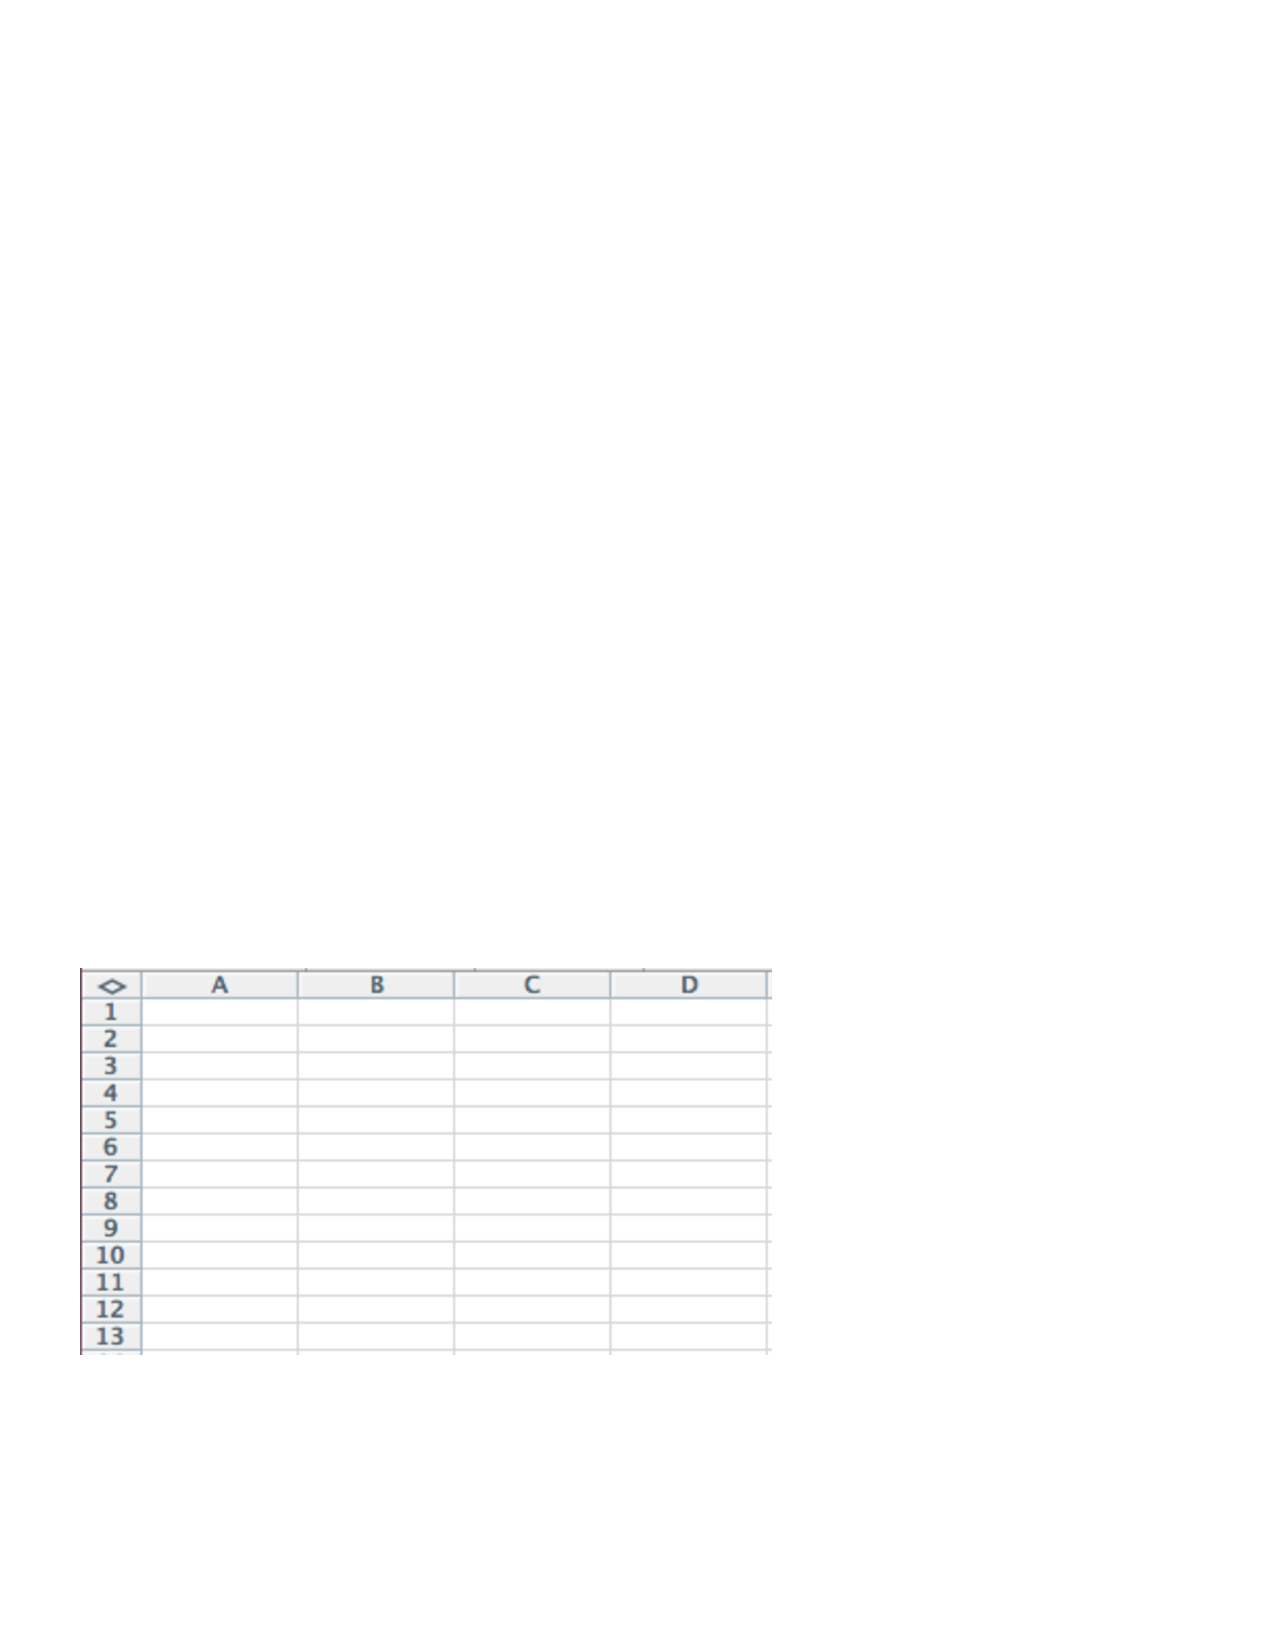
\includegraphics[width=.7\linewidth]{LabmanualFigures/Excel1.pdf}
      \caption{The excel window}
      \label{fig:excelwindow}
\end{figure}

\subsection{Inputting data}

Type or paste individual numbers or letters into individual cells, and then press return.

\begin{figure}
      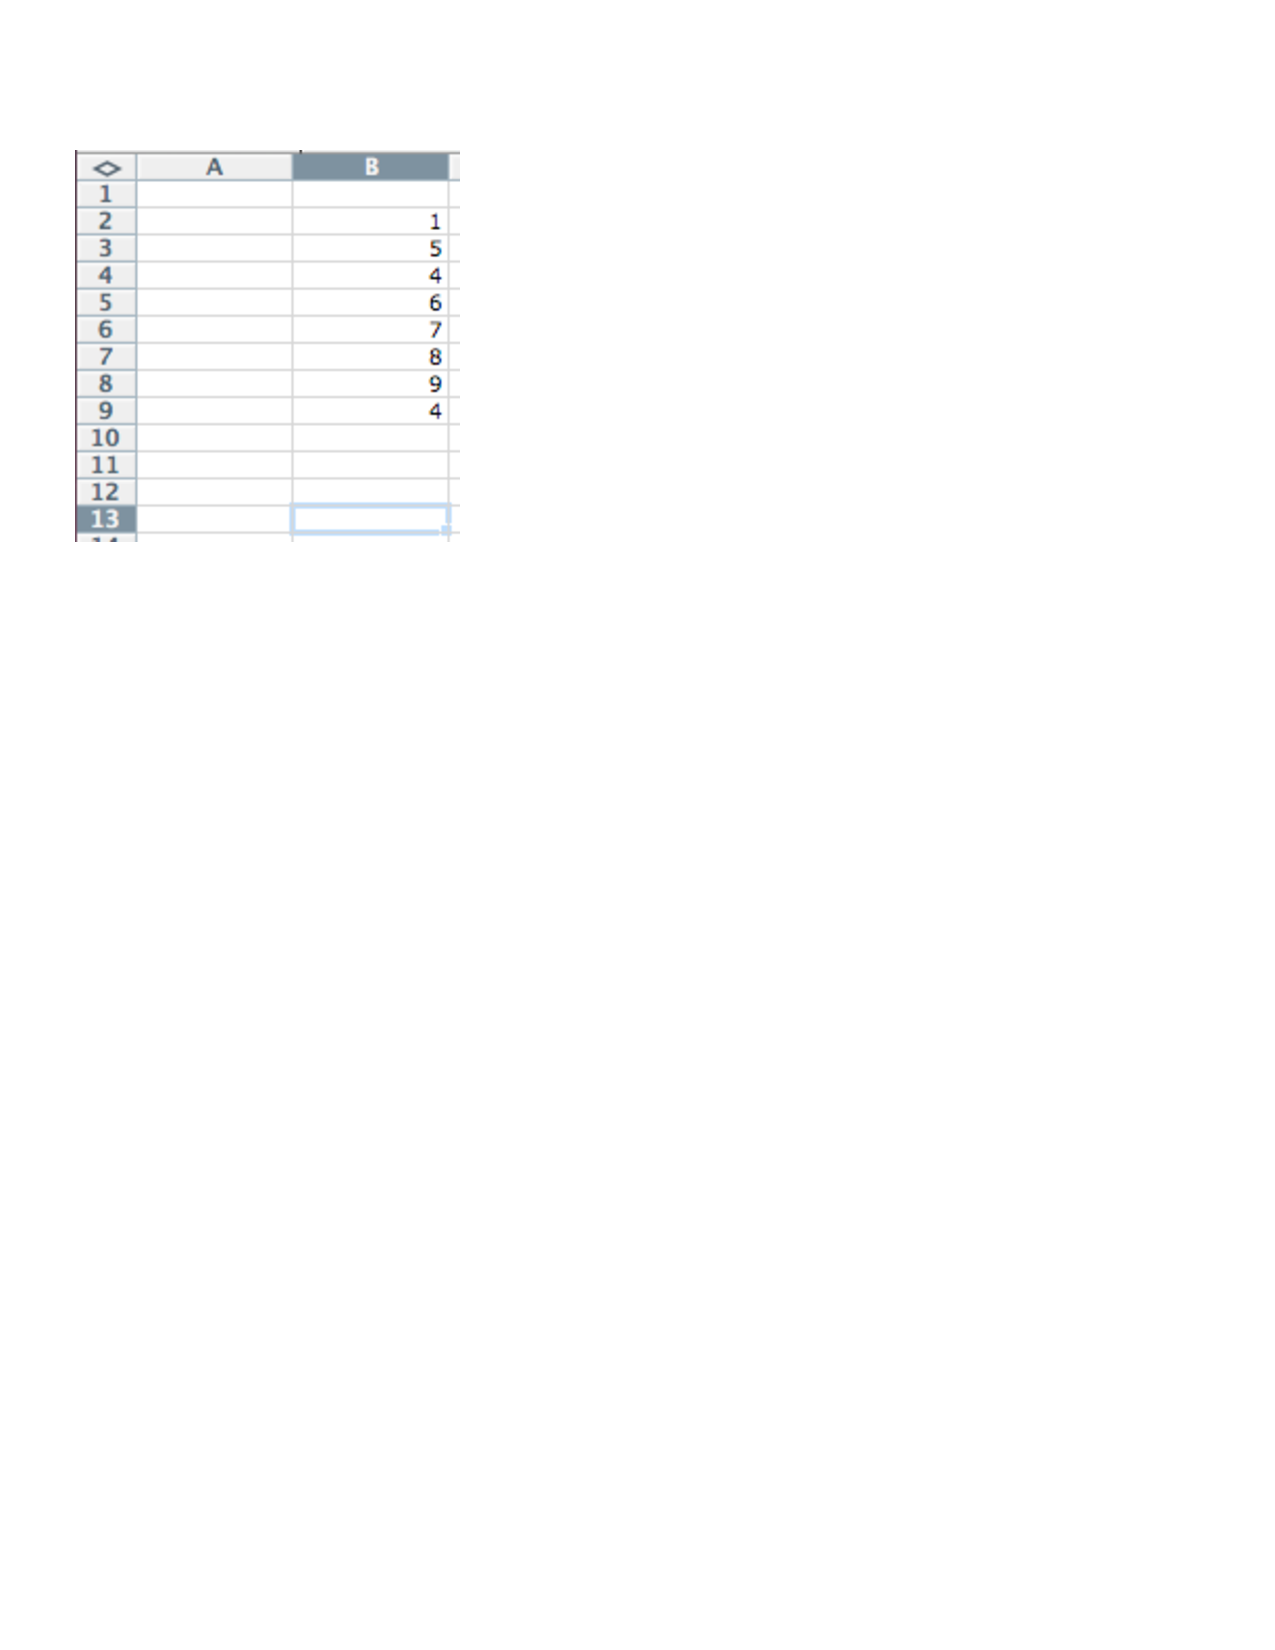
\includegraphics[width=.5\linewidth]{LabmanualFigures/Excel2.pdf}
      \caption{Inputting data}
      \label{fig:excel2}
\end{figure}

\subsection{Addressing cells}

Excel uses a Letter-Number system to address or point to specific cells. As you can see, all of the numbers in this example have been added to rows 2-9 in Column B. Using the Letter- Number system, the B2=1, B3=5, B4=4, B6=7, and so on.


\subsection{Setting one cell to equal another}

\begin{figure}
      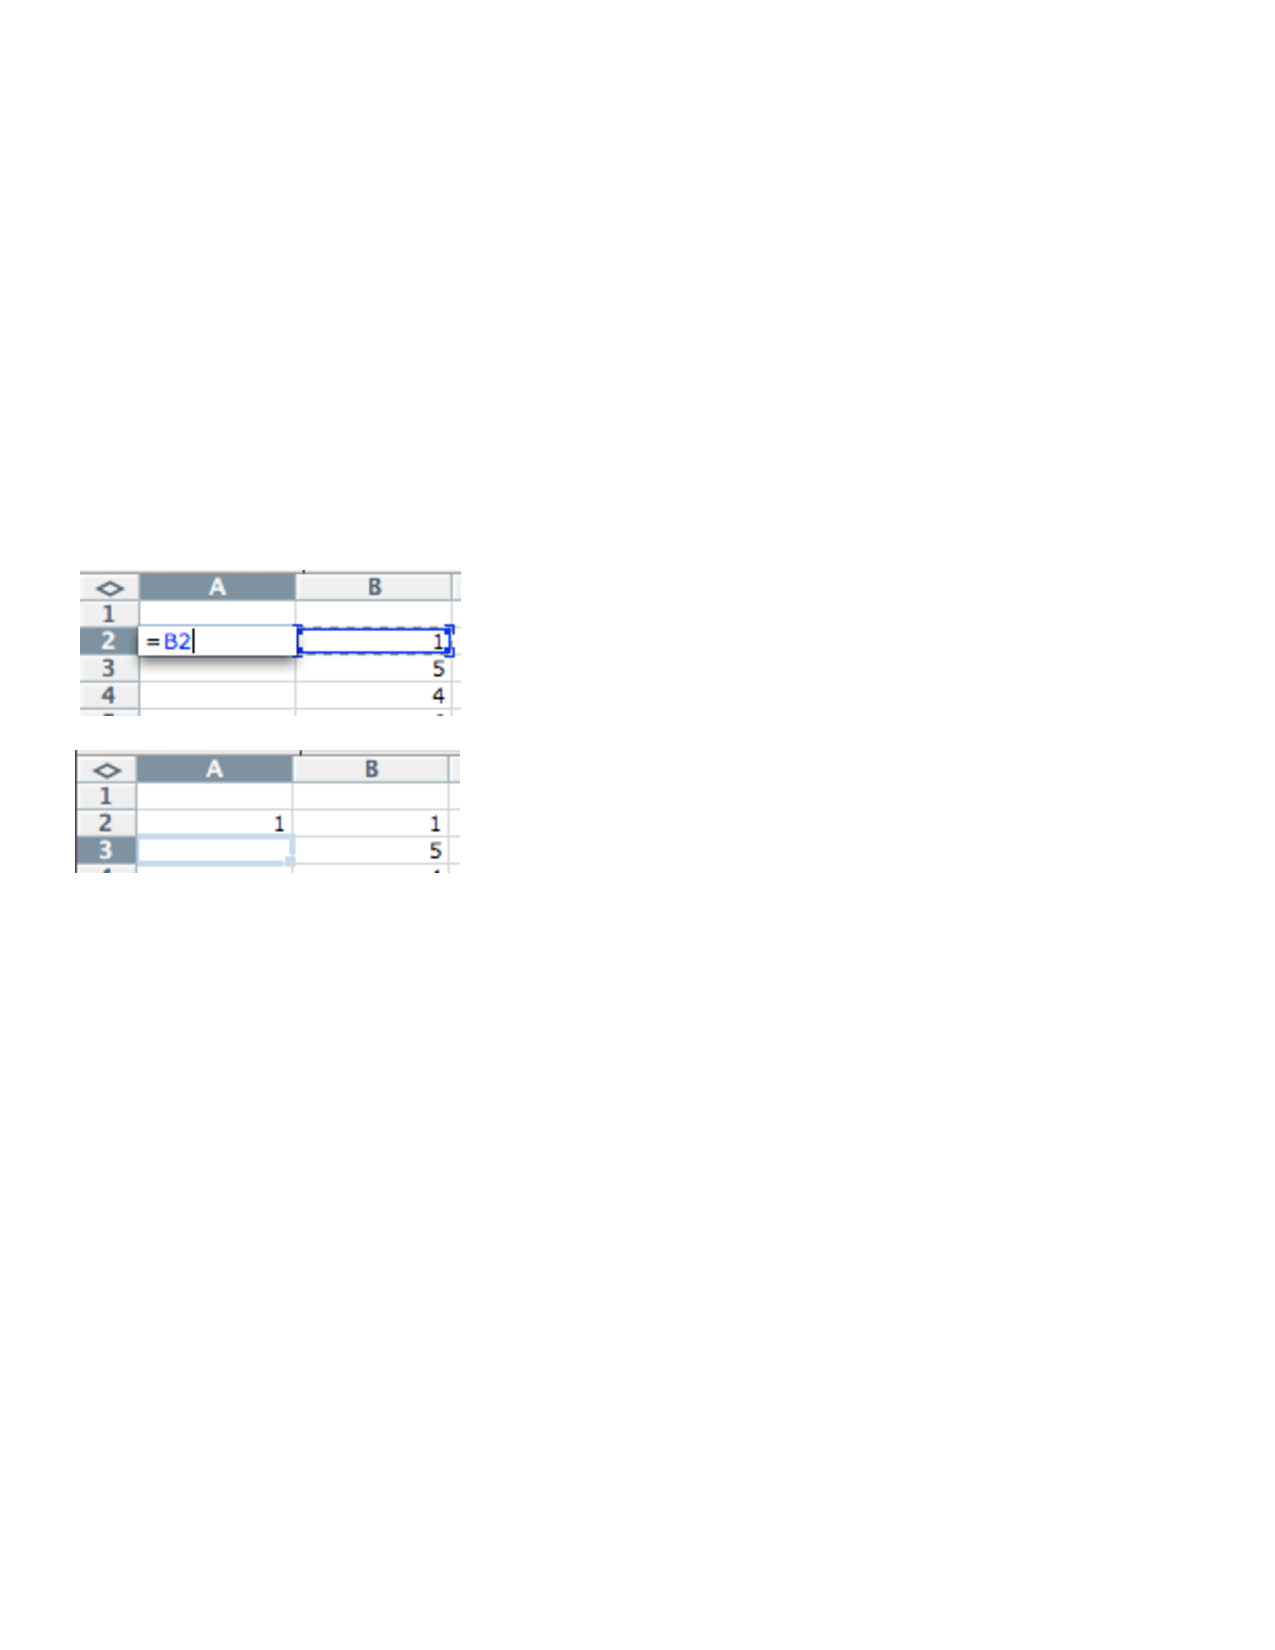
\includegraphics[width=.5\linewidth]{LabmanualFigures/Excel3.pdf}
      \caption{Making one cell equal another}
      \label{fig:excel3}
\end{figure}

If you click on an empty cell, you can make this cell have the same contents as another cell by typing the (=) sign, then clicking on the cell you want to duplicate.
E.g., click on A2, type (=), then click on B2. B2 initially had a 1 in it, now when you press enter, cell A2 will also have a 1 in it. Now if you change the contents of B2 to another number (say 5), the contents of A2 will also change to 5.
Note: this trick becomes handy later on to help you quickly manipulate data in excel

\subsection{Adding cells together, and copying commands across other cells}

\begin{figure}
      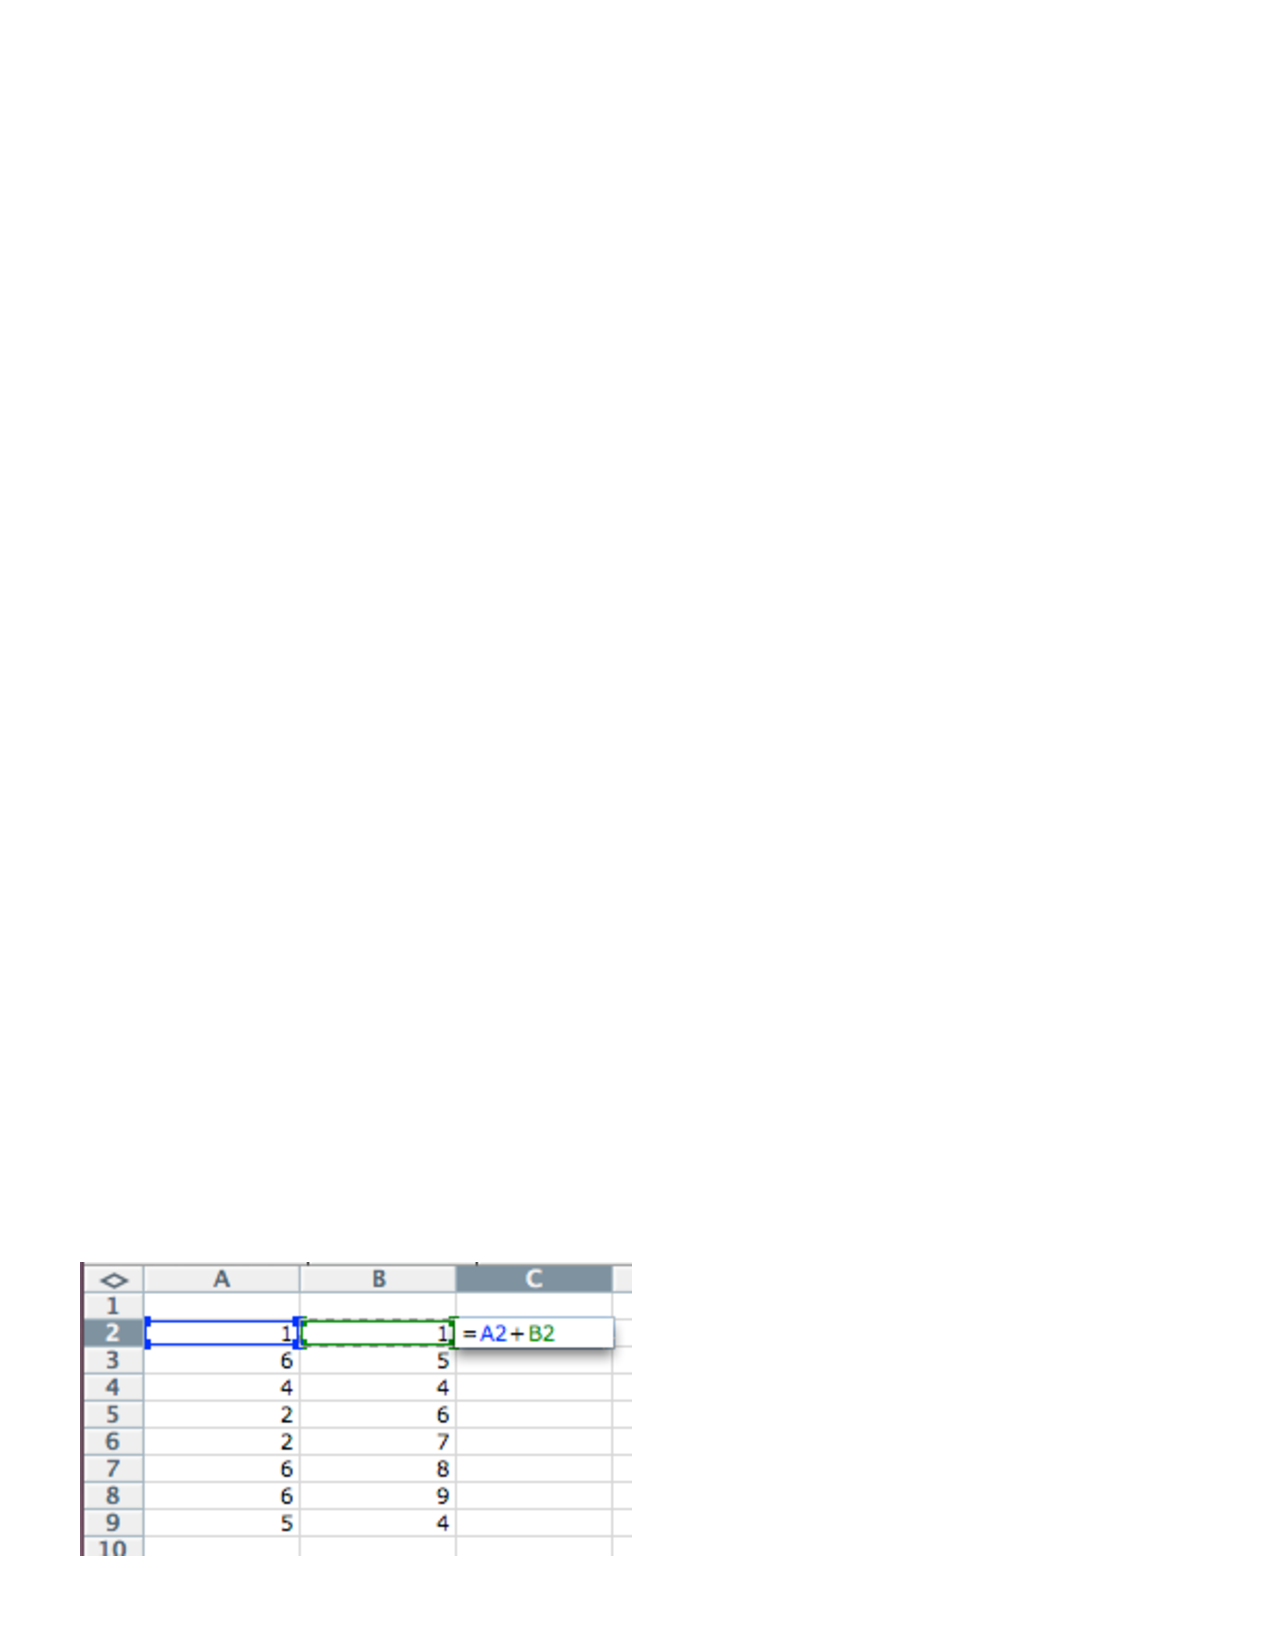
\includegraphics[width=.5\linewidth]{LabmanualFigures/Excel4.pdf}
      \caption{Adding}
      \label{fig:excel4}
\end{figure}

Let's say you had two columns of numbers. For each row you want to compute the sum of the first and second number (e.g., the first two numbers are 1 and 1, you want to add them together to get 2.
Click on a new column (C2) and type the equal sign =
Now click on A2 (which contains 1) once with the mouse, and then click on B2 (which also contains 1). Now the formula in C2 will automatically contain =A2+B2
When you press enter the two numbers will be summed, and the answer in C2 with be 2.

\begin{figure}
      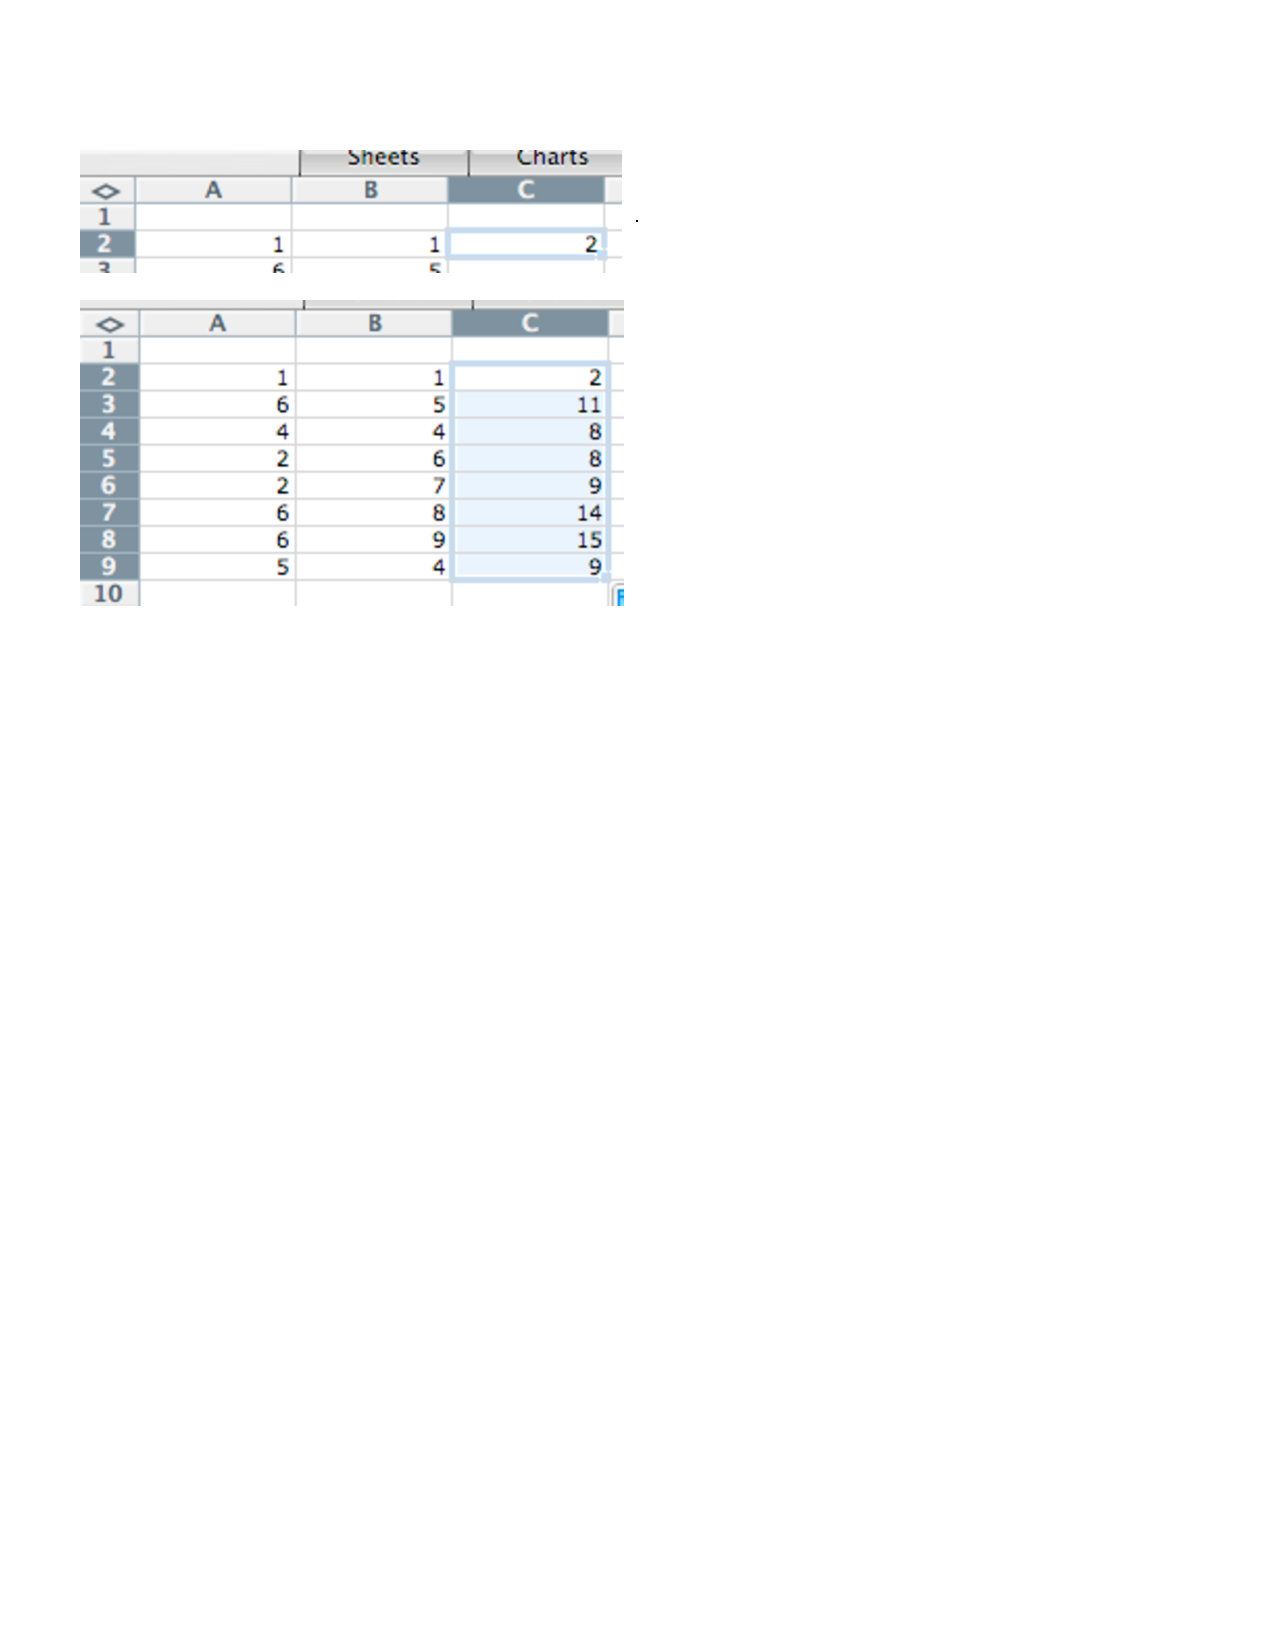
\includegraphics[width=.5\linewidth]{LabmanualFigures/Excel5.pdf}
      \caption{Applying across cells}
      \label{fig:excel5}
\end{figure}

If you want to do the same operation for all of the rows, all you have to do is click on C2. Notice there is a little blue square at the bottom right hand corner of the cell.
   

\subsection{Using a formula to add two numbers together}
You can do the same addition operation from above by using the sum formula. In this example you would click on C2, then type =sum(
Then you need to tell excel the range of columns and rows that you want to sum over. In this case you can just click on A2, and drag across to B2. This will make a temporary blue rectangle, which represents the cells that will be summed together
Complete the formula by using the )
Then press enter, and you will get the answer. 

\begin{figure}
      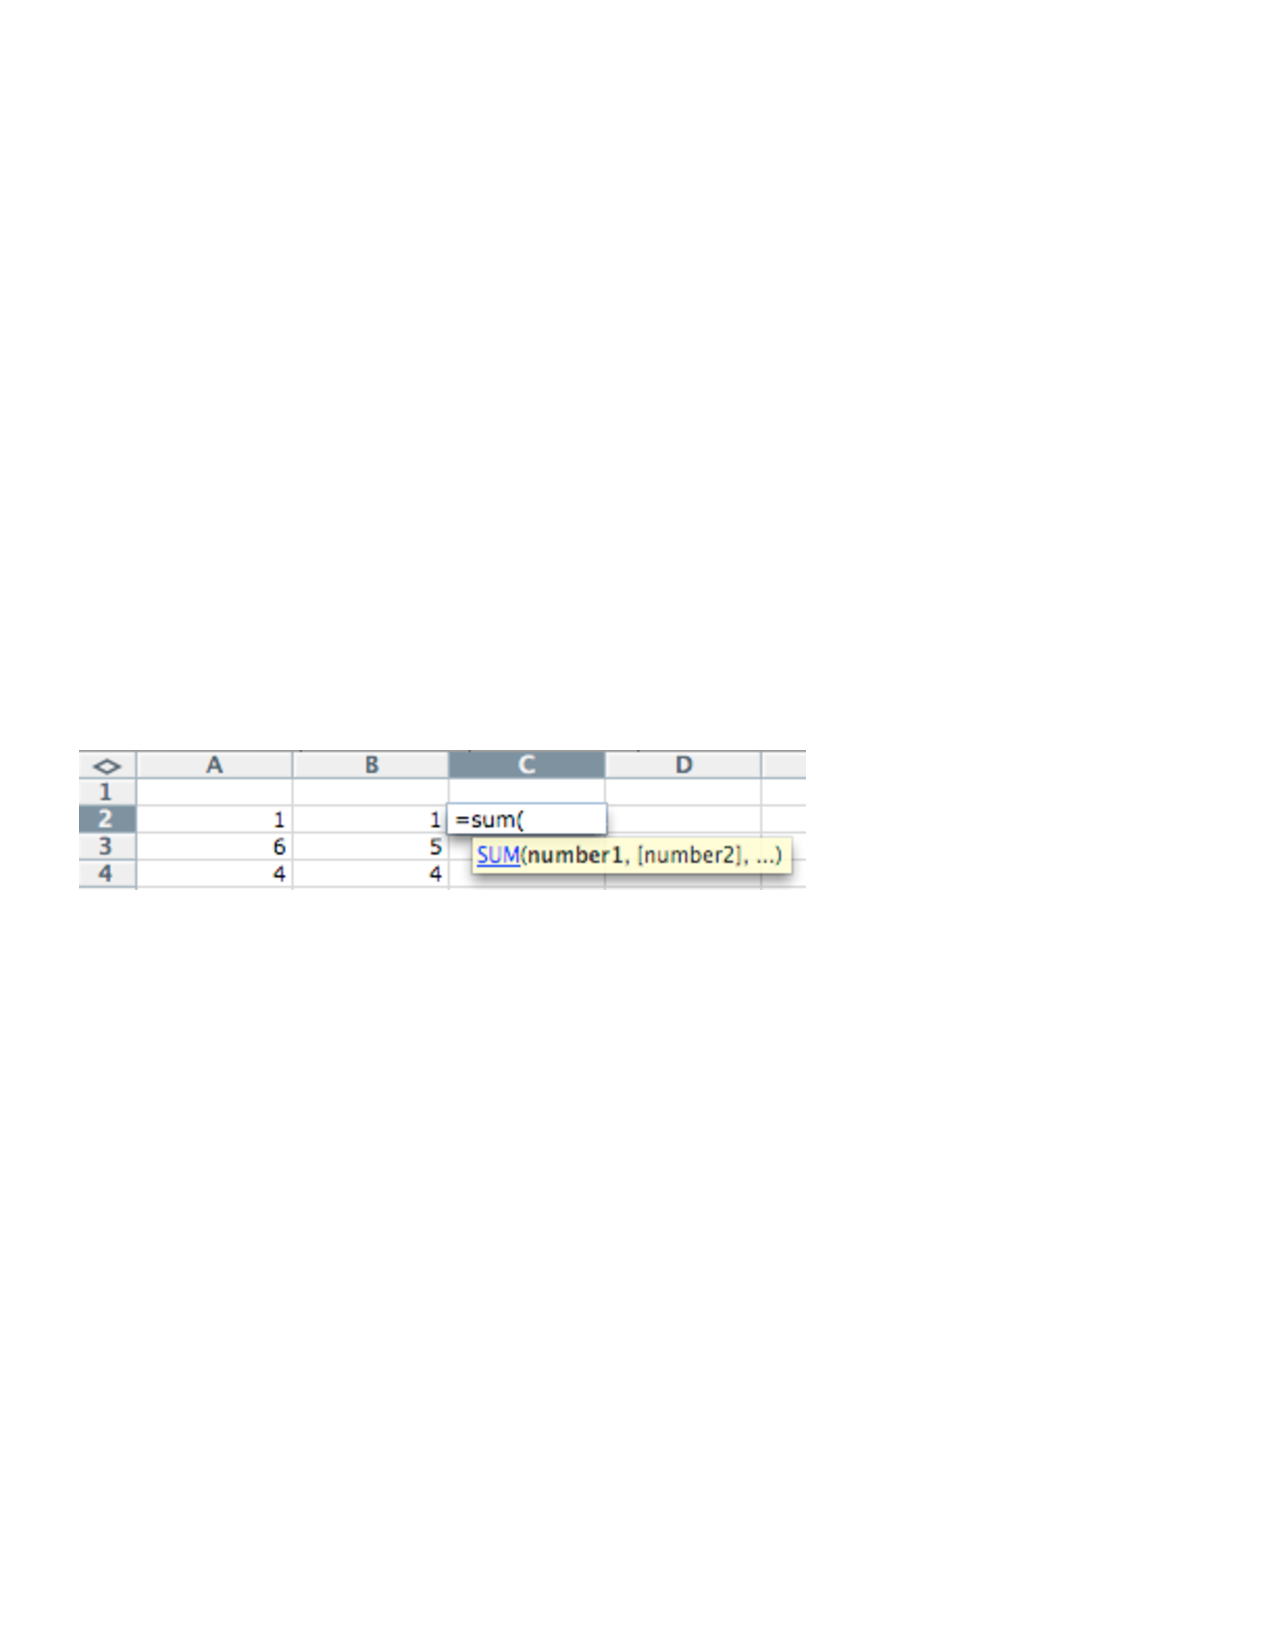
\includegraphics[width=.5\linewidth]{LabmanualFigures/Excel6.pdf}
      \caption{Adding using the sum formula}
      \label{fig:excel6}
\end{figure}

You can also copy this formula down across the other cells in the same way as above
If you click on the little square, then drag down, the formula will be applied to each of the rows.
And, then you have all the answers without having to enter the formula separately for each row.

\begin{figure}
      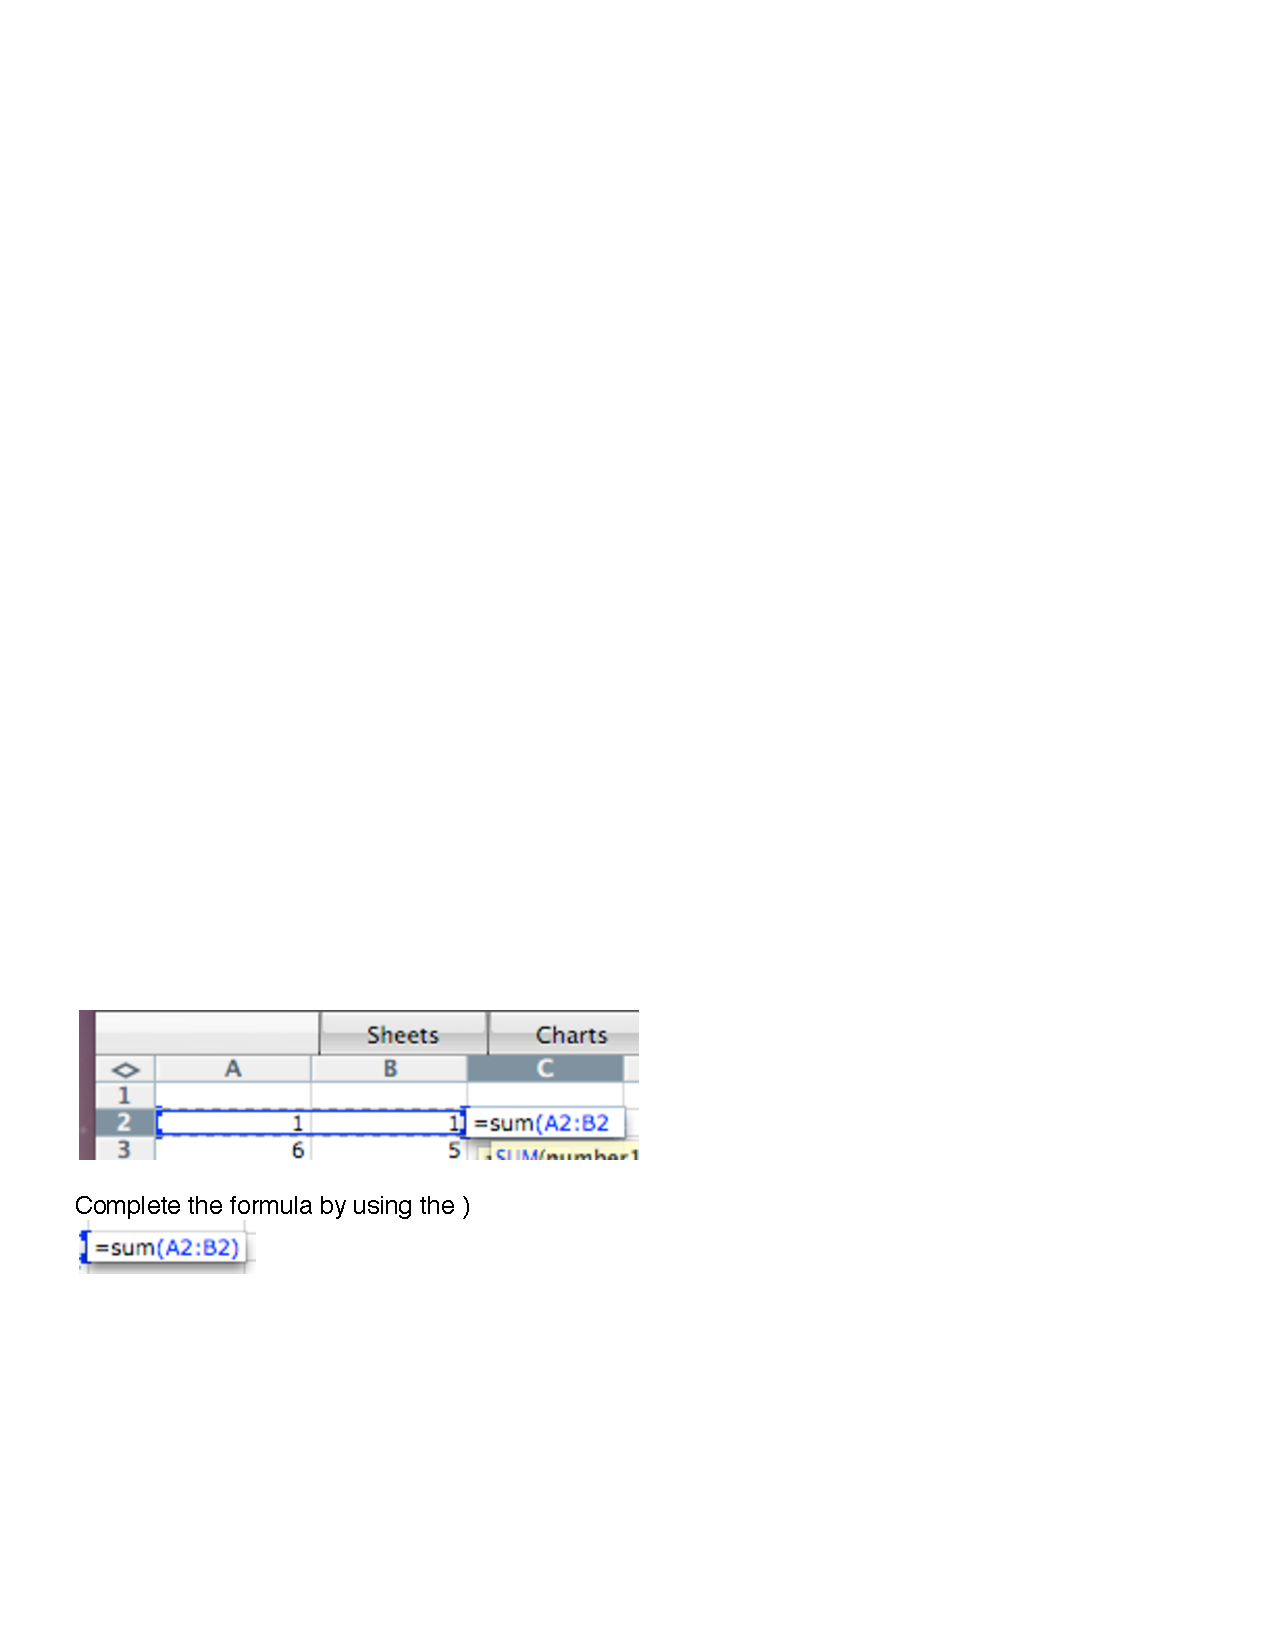
\includegraphics[width=.5\linewidth]{LabmanualFigures/Excel7.pdf}
      \caption{Completing the formula}
      \label{fig:excel7}
\end{figure}    

\subsection{Getting an average}

Using the same method as the sum formula, you can also compute the mean of a set of numbers by using the average function instead of the sum function. The process is the same. Select a cell, type =average( then select the cells you want (in the example B2:B9) and press enter.

\begin{figure}
      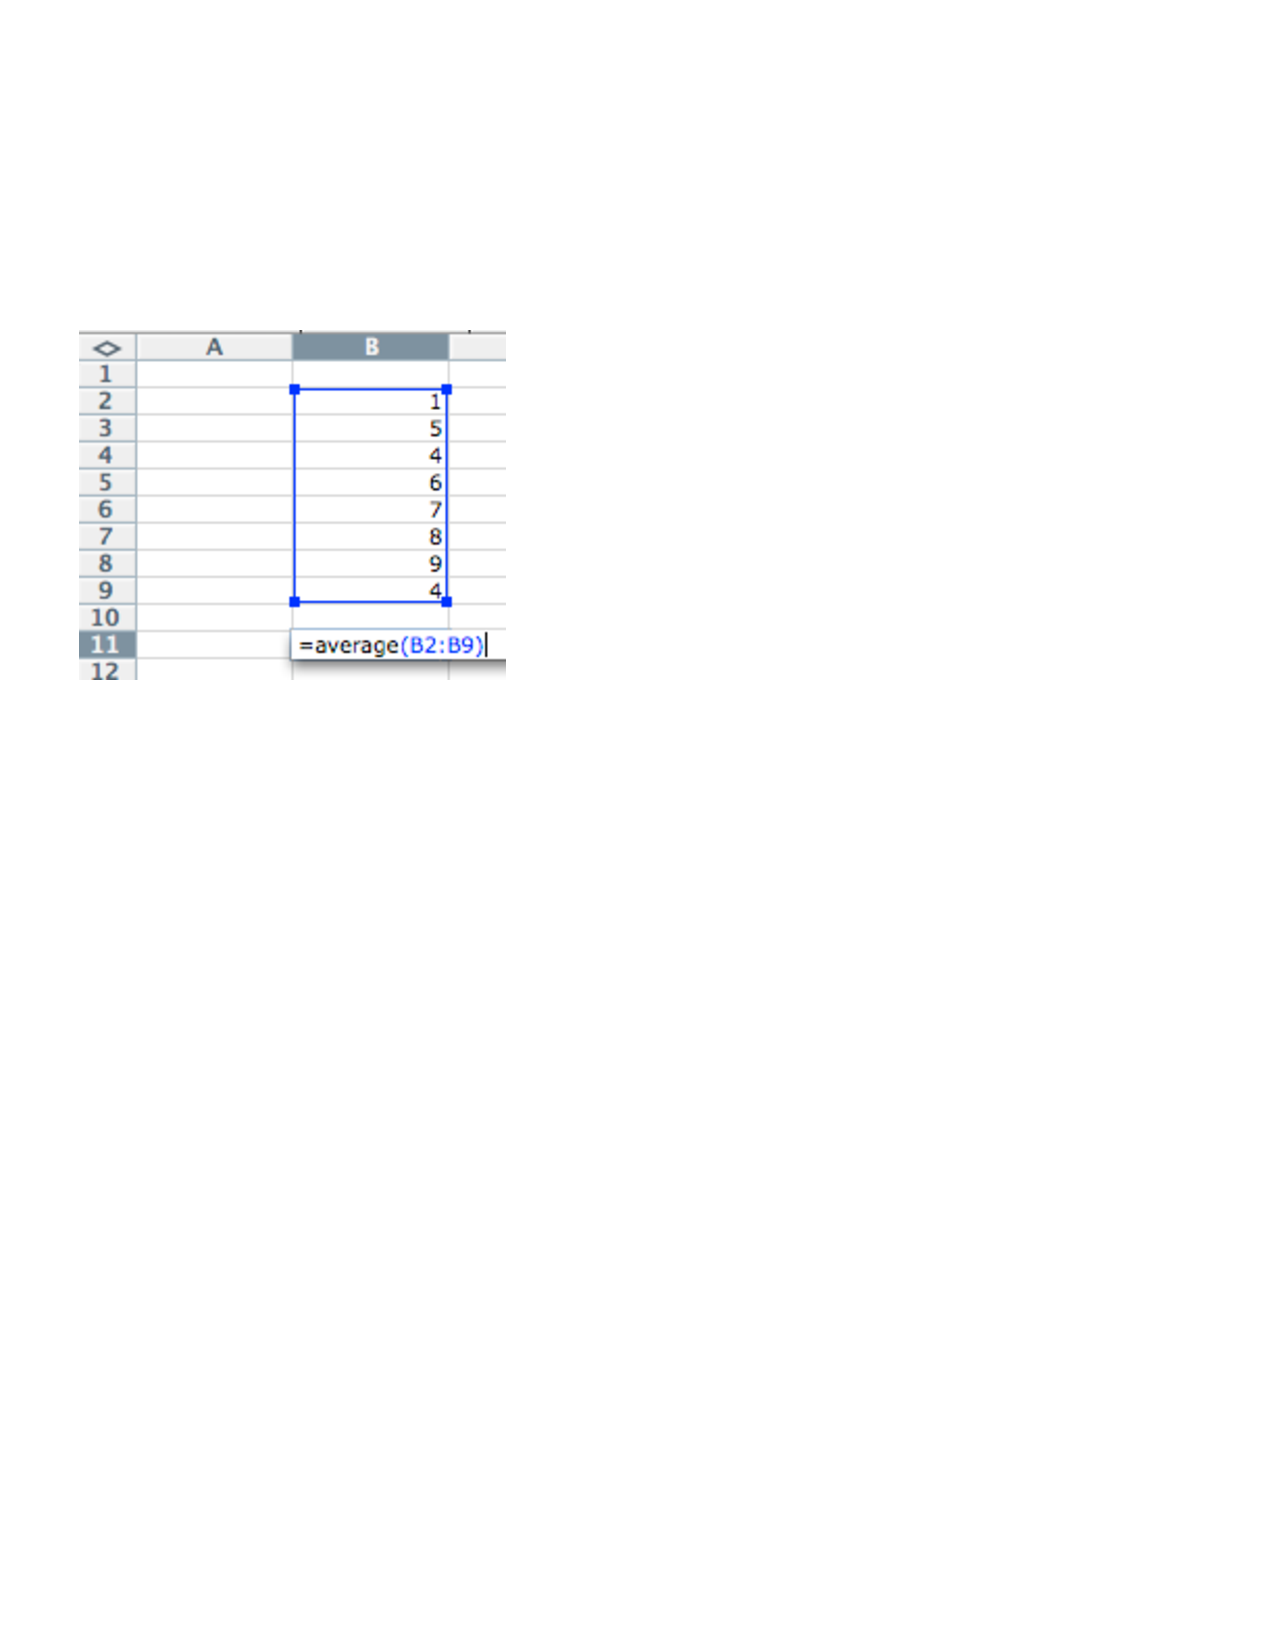
\includegraphics[width=.5\linewidth]{LabmanualFigures/Excel8.pdf}
      \caption{The average formal}
      \label{fig:excel8}
\end{figure}

\subsection{Other formulas}

\begin{itemize}
\item Max – finds the biggest number
\item Min- finds the smallest number
\item Stdev- computes the standard deviation
\item Countif – counts the number of times a specific value occurs
\end{itemize}

Excel has a dictionary of other functions that may be useful, you can look them using help, or using insert: function, from the menu.


\subsection{Selecting a range of cells}
Formulas usually require you to enter a range of cells to compute. The format is put the upperleftmost cell first (e.g., A2), and then the bottomrightmost cell last (e.g., C9). So, A2:C9 would signify the
following rectangle.

\begin{figure}
      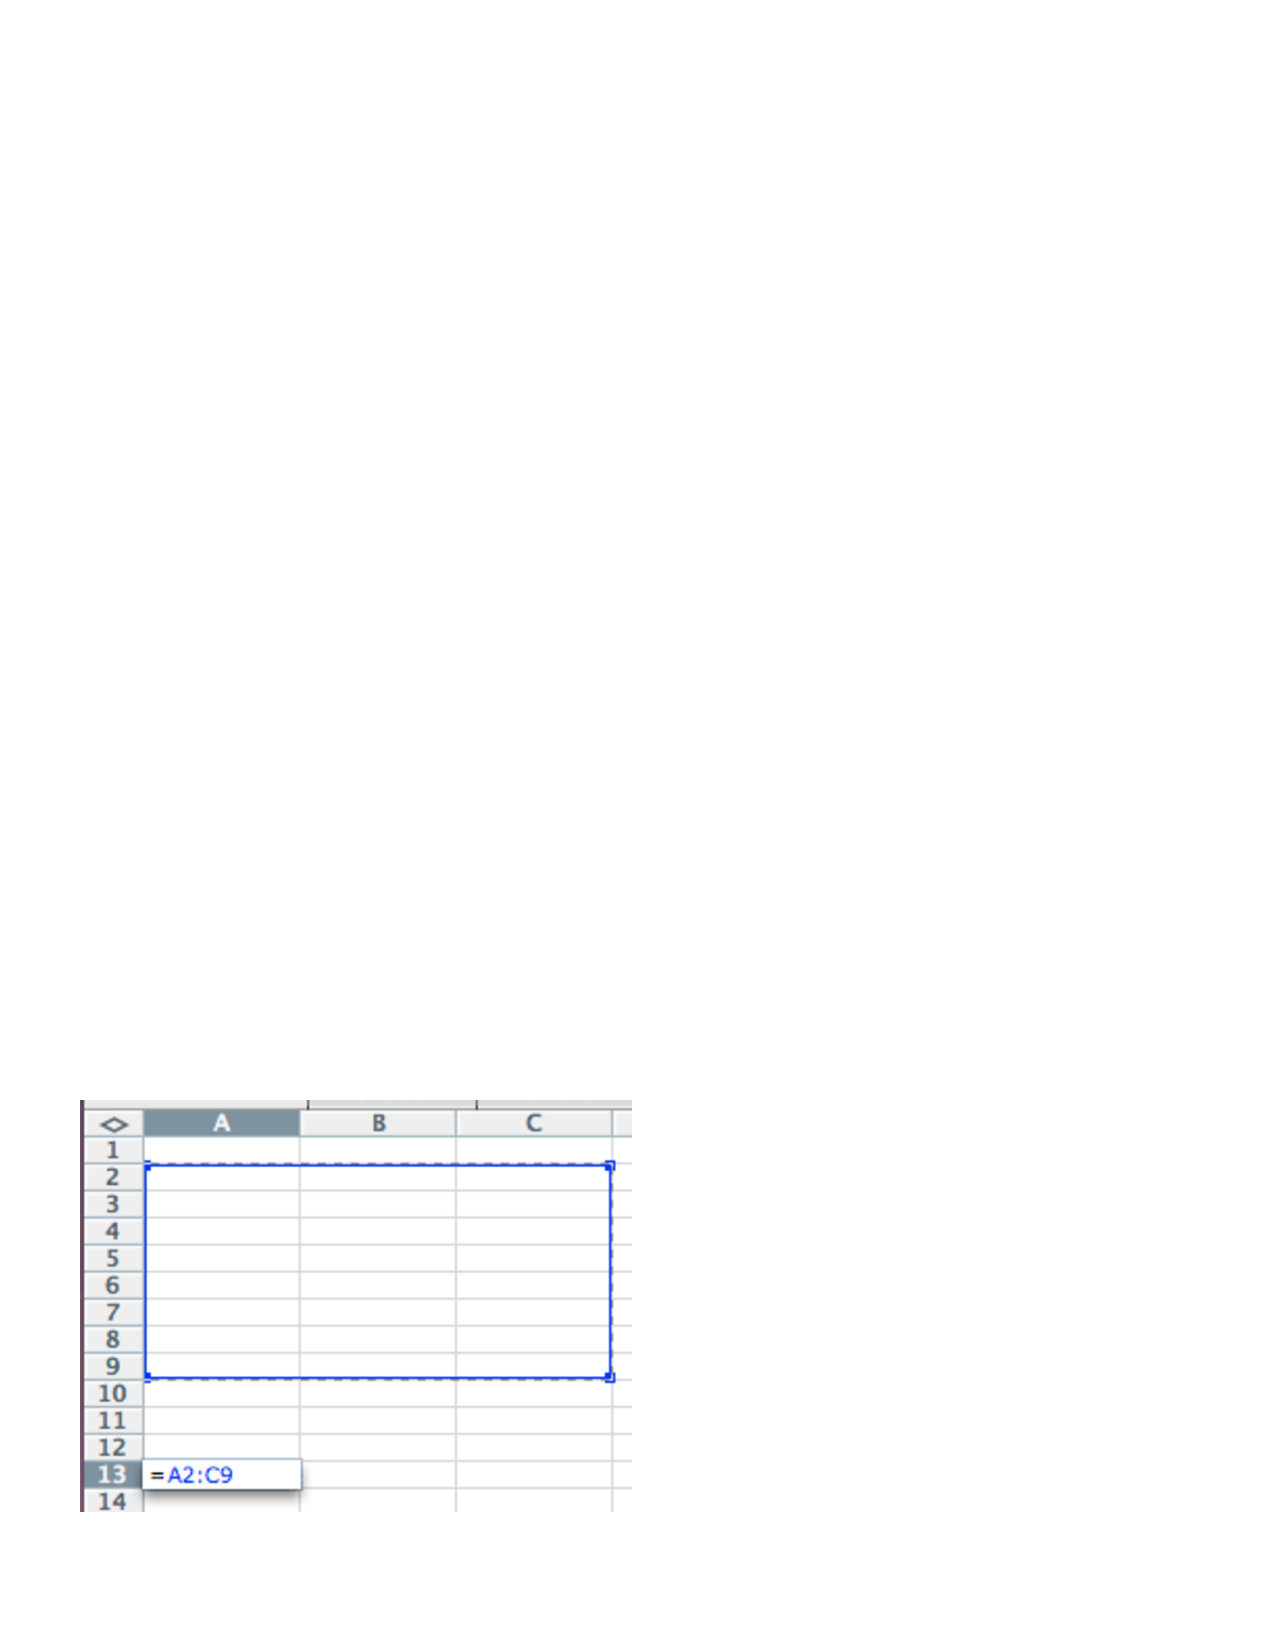
\includegraphics[width=.5\linewidth]{LabmanualFigures/Excel9.pdf}
      \caption{selecting a range}
      \label{fig:excel9}
\end{figure}
  

\subsection{Copying a formula to another cell: relative coordinates}

If you were to now select cell A13 it would have the formula =A2:C9 inside. If you copied this cell, and then pasted it into the cell beside it A14, Excel would automatically move the rectangle over one. This is because without further specification, excel always treats cells in relative coordinates.

\begin{figure}
      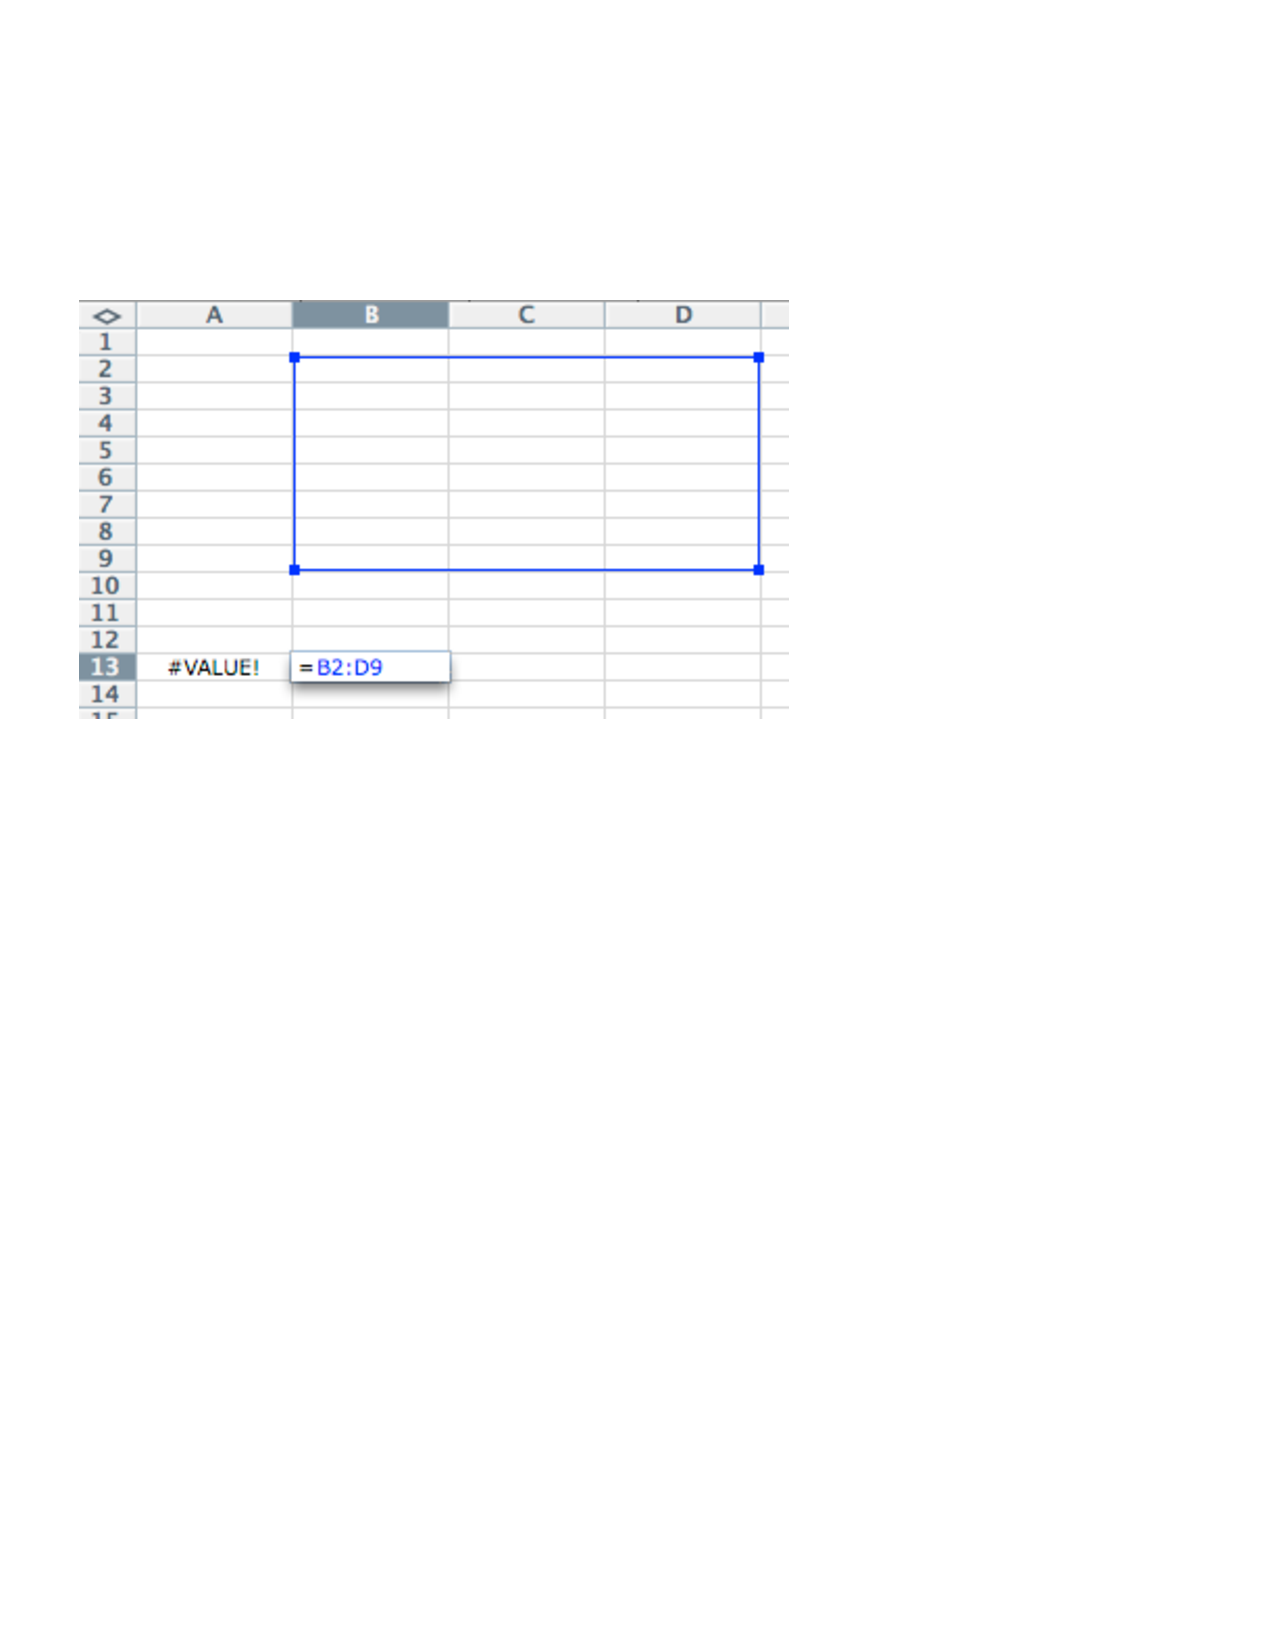
\includegraphics[width=.5\linewidth]{LabmanualFigures/Excel10.pdf}
      \caption{Relative coordinates}
      \label{fig:excel10}
\end{figure}
 

\subsection{Absolute coordinates}
You can control whether or not excel uses relative coordinates. When you set the range you can insert the \$ sign to make sure that excel holds the rectangle in place.
For example:
A13 =A2:C9
-this formula has no \$s, as in the above example, if you copy this formula to another cell say
B13, then B13=B2:D9, and not the original A2:C9
A13=\$A\$2:\$C\$9
-This formula has \$s infront of both letter and number for each cell in the rectangle. Now, when
the formula is copied to another cell, the original rectangle will be used. E.g., B13=A2:C9 You can set the only columns or the row or both to absolute coordinates using the \$ sign.
 

\subsection{Sorting data}

\begin{figure}
      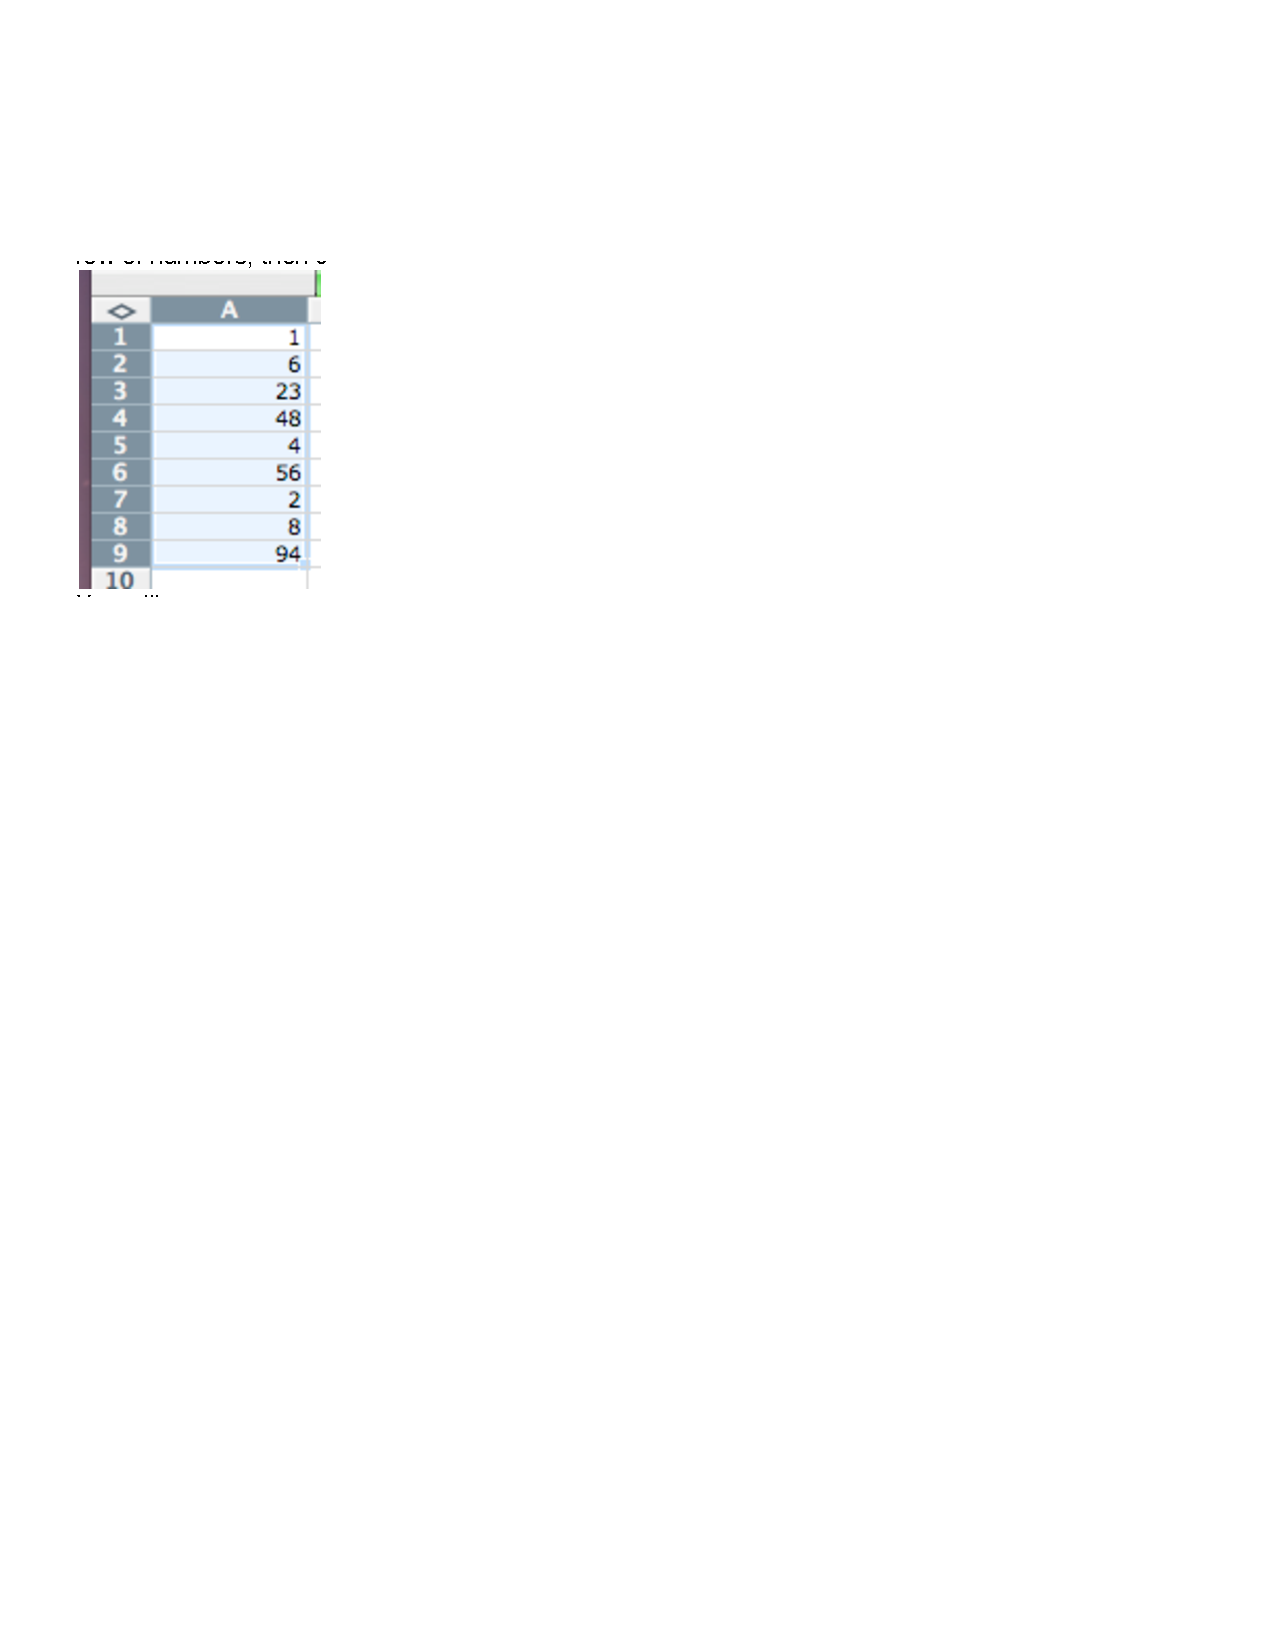
\includegraphics[width=.5\linewidth]{LabmanualFigures/Excel11.pdf}
      \caption{Some numbers to sort}
      \label{fig:excel11}
\end{figure}
 

If you had a bunch of numbers in random order, you could easily sort them by selecting the column or row of numbers, then click on Data from the menu, and choose sort:

\begin{figure}
      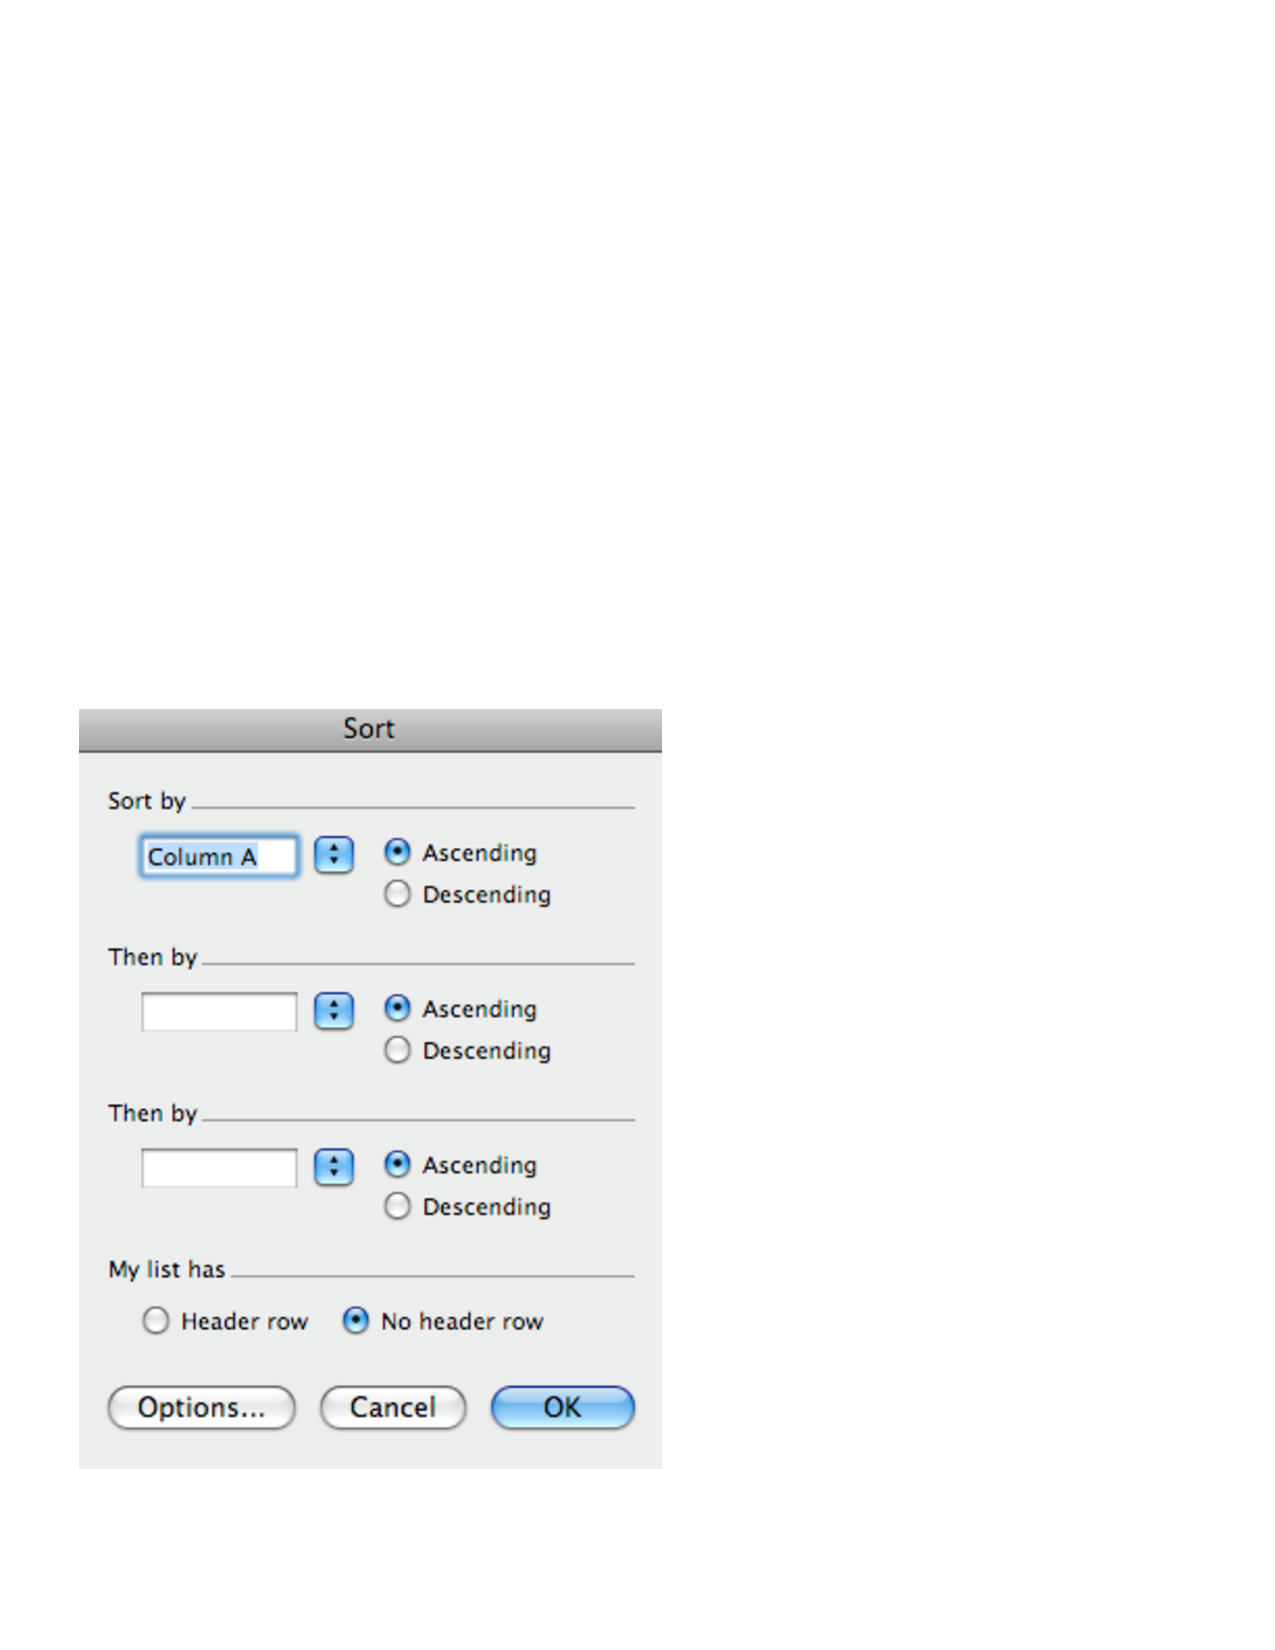
\includegraphics[width=.5\linewidth]{LabmanualFigures/Excel12.pdf}
      \caption{Sorting}
      \label{fig:excel12}
\end{figure}
 


 
You will see a menu something like this. You can choose to sort the current column ascending (smallest to largest) or descending (largest to smallest). Click OK and the data will be rearranged in order.
  

\subsection{Making a histogram}

\begin{figure}
      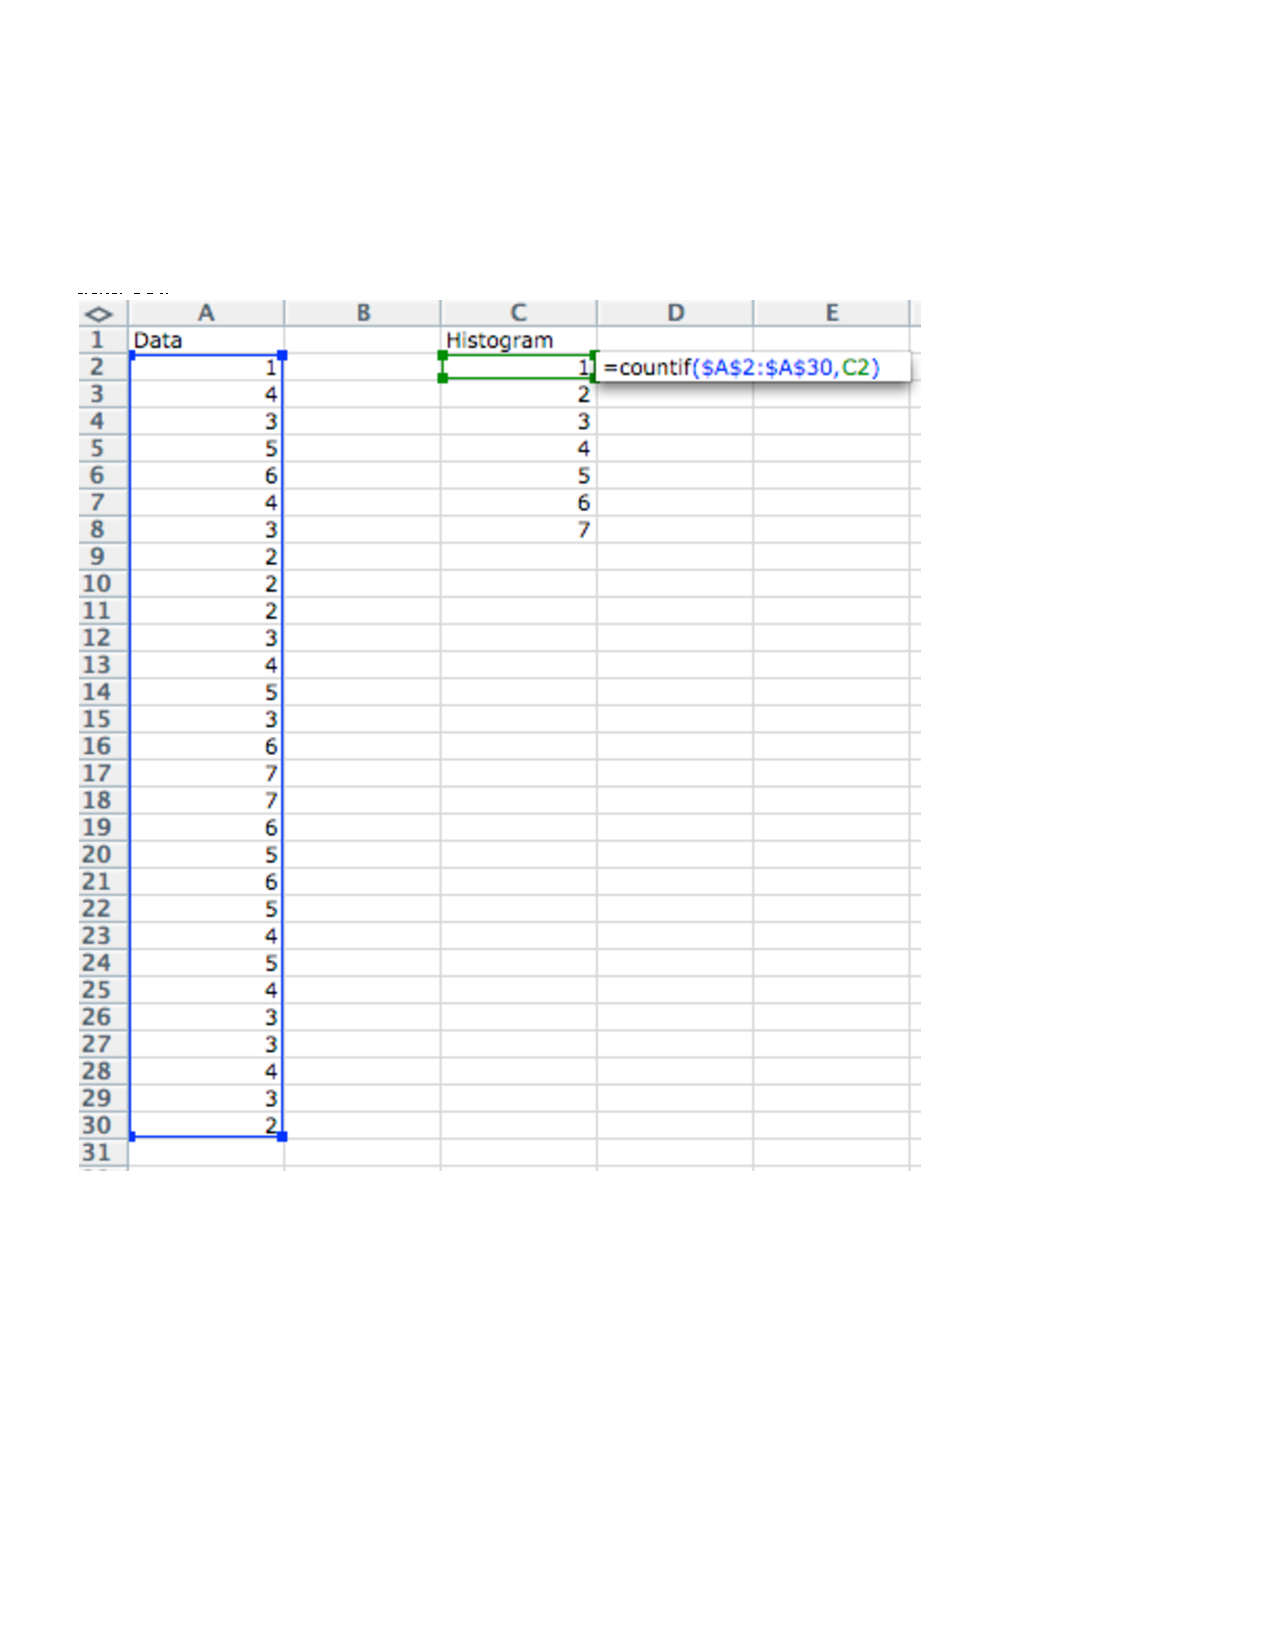
\includegraphics[width=.7\linewidth]{LabmanualFigures/Excel13.pdf}
      \caption{Making a histogram}
      \label{fig:excel13}
\end{figure}
 


If you want to know how many responses occurred for a particular range of values you can create a histogram. The following example is a very simple way to count individual categories of values in a data set.
Column A has the example data. In column C, I created cells with values ranging from 1 to 7 (Cells C2 : C8). In cell D2, I typed in the countif(range,value) formula. The range refers to the selected data (\$A\$2:\$A\$30). 

Note, there are \$ signs used before the letter and numbers so that the selected data will be the same when the formula is copied. In this case, it is the value 1, which is in Cell C2. The value refers to the entity that is being counted. When you press enter, excel will compute the number of times that 1 appears in the data. You can now drag cell (D2) with the formula down, and it will be used to count the rest of the numbers.
 


\subsection{Making a table}

\begin{figure}
      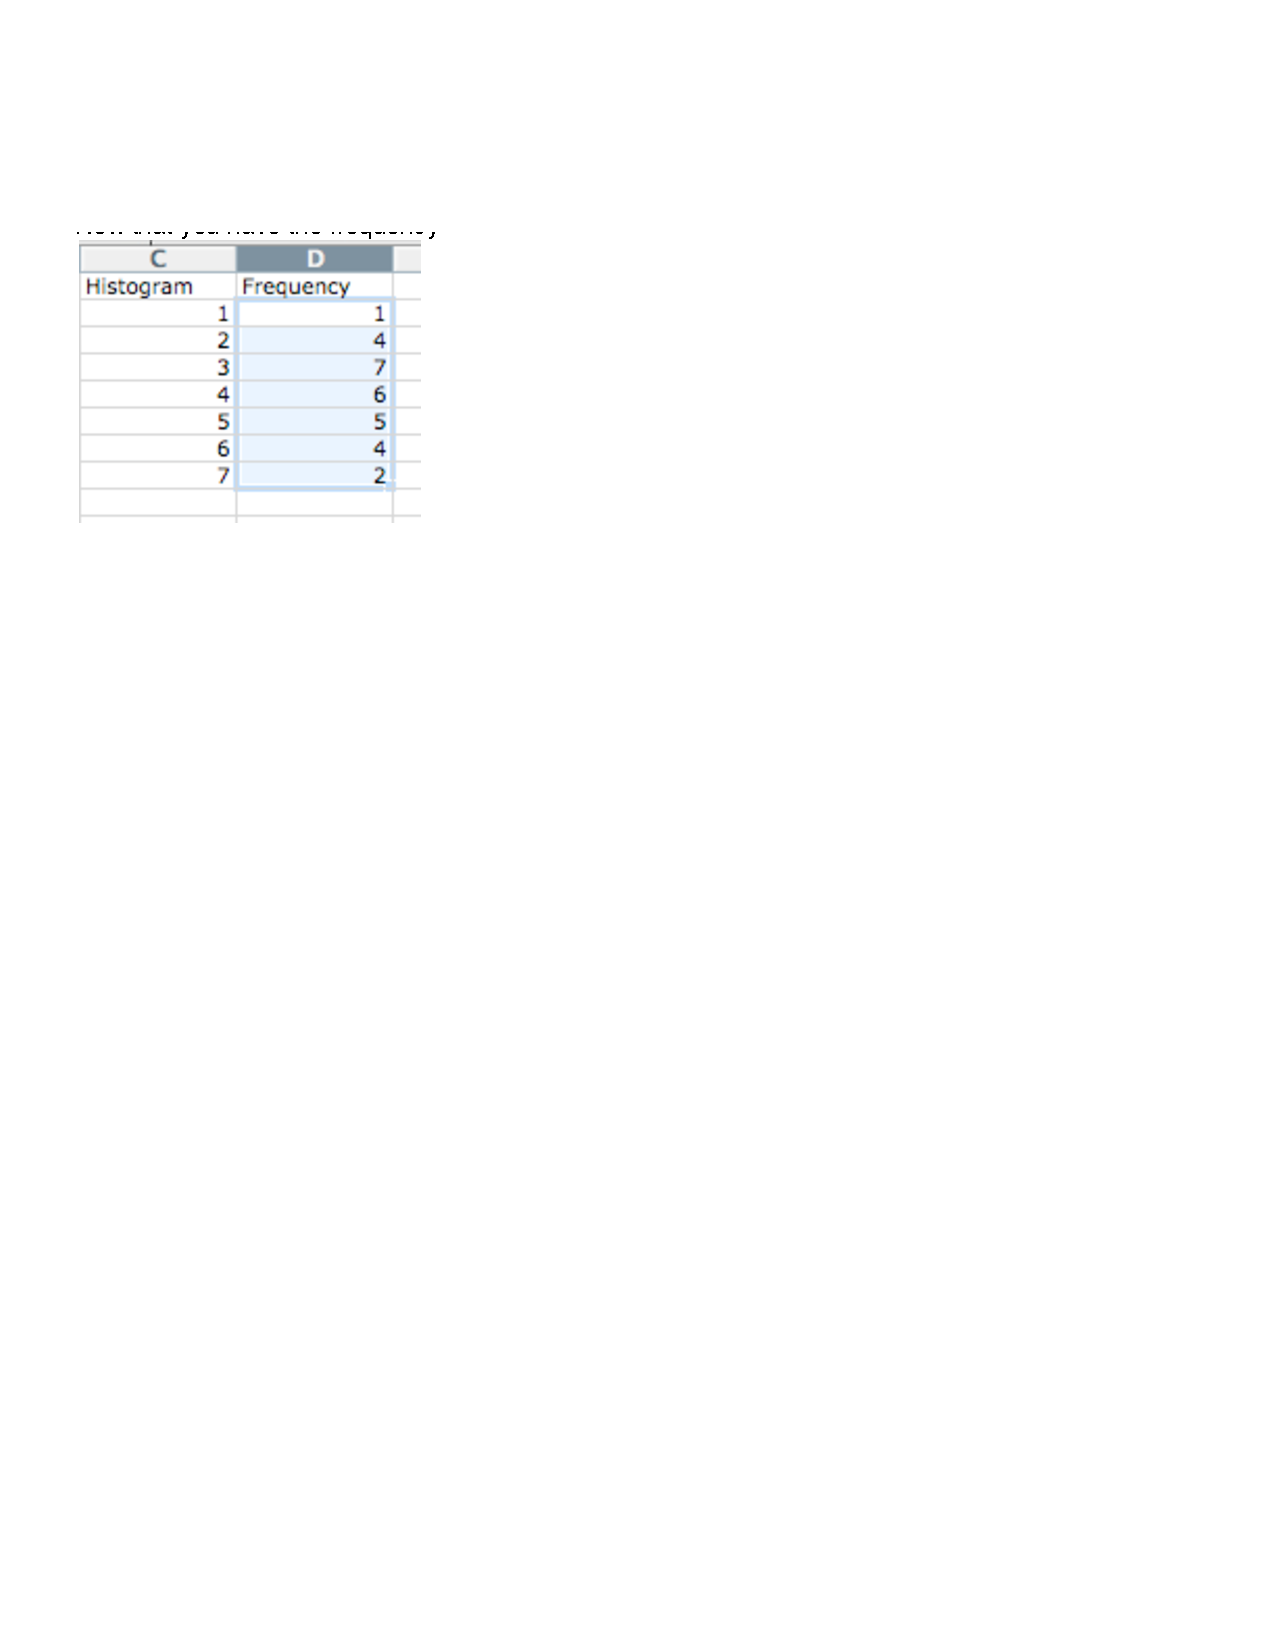
\includegraphics[width=.7\linewidth]{LabmanualFigures/Excel14.pdf}
      \caption{Making a table}
      \label{fig:excel14}
\end{figure}
 
Now that you have the frequency of each of the values from 1-7.
You can make a graph by selecting the column with the frequencies in it, and then click on INSERT, from the menu, and choose chart. Select a column chart, and then you will see:
You can then edit this chart. You should insert a title for the figure, an x-axis label (e.g., the numbers on the bottom represent different categories from the data), and a y-axis label (the numbers on the left side represent the frequency count).
 

\begin{figure}
      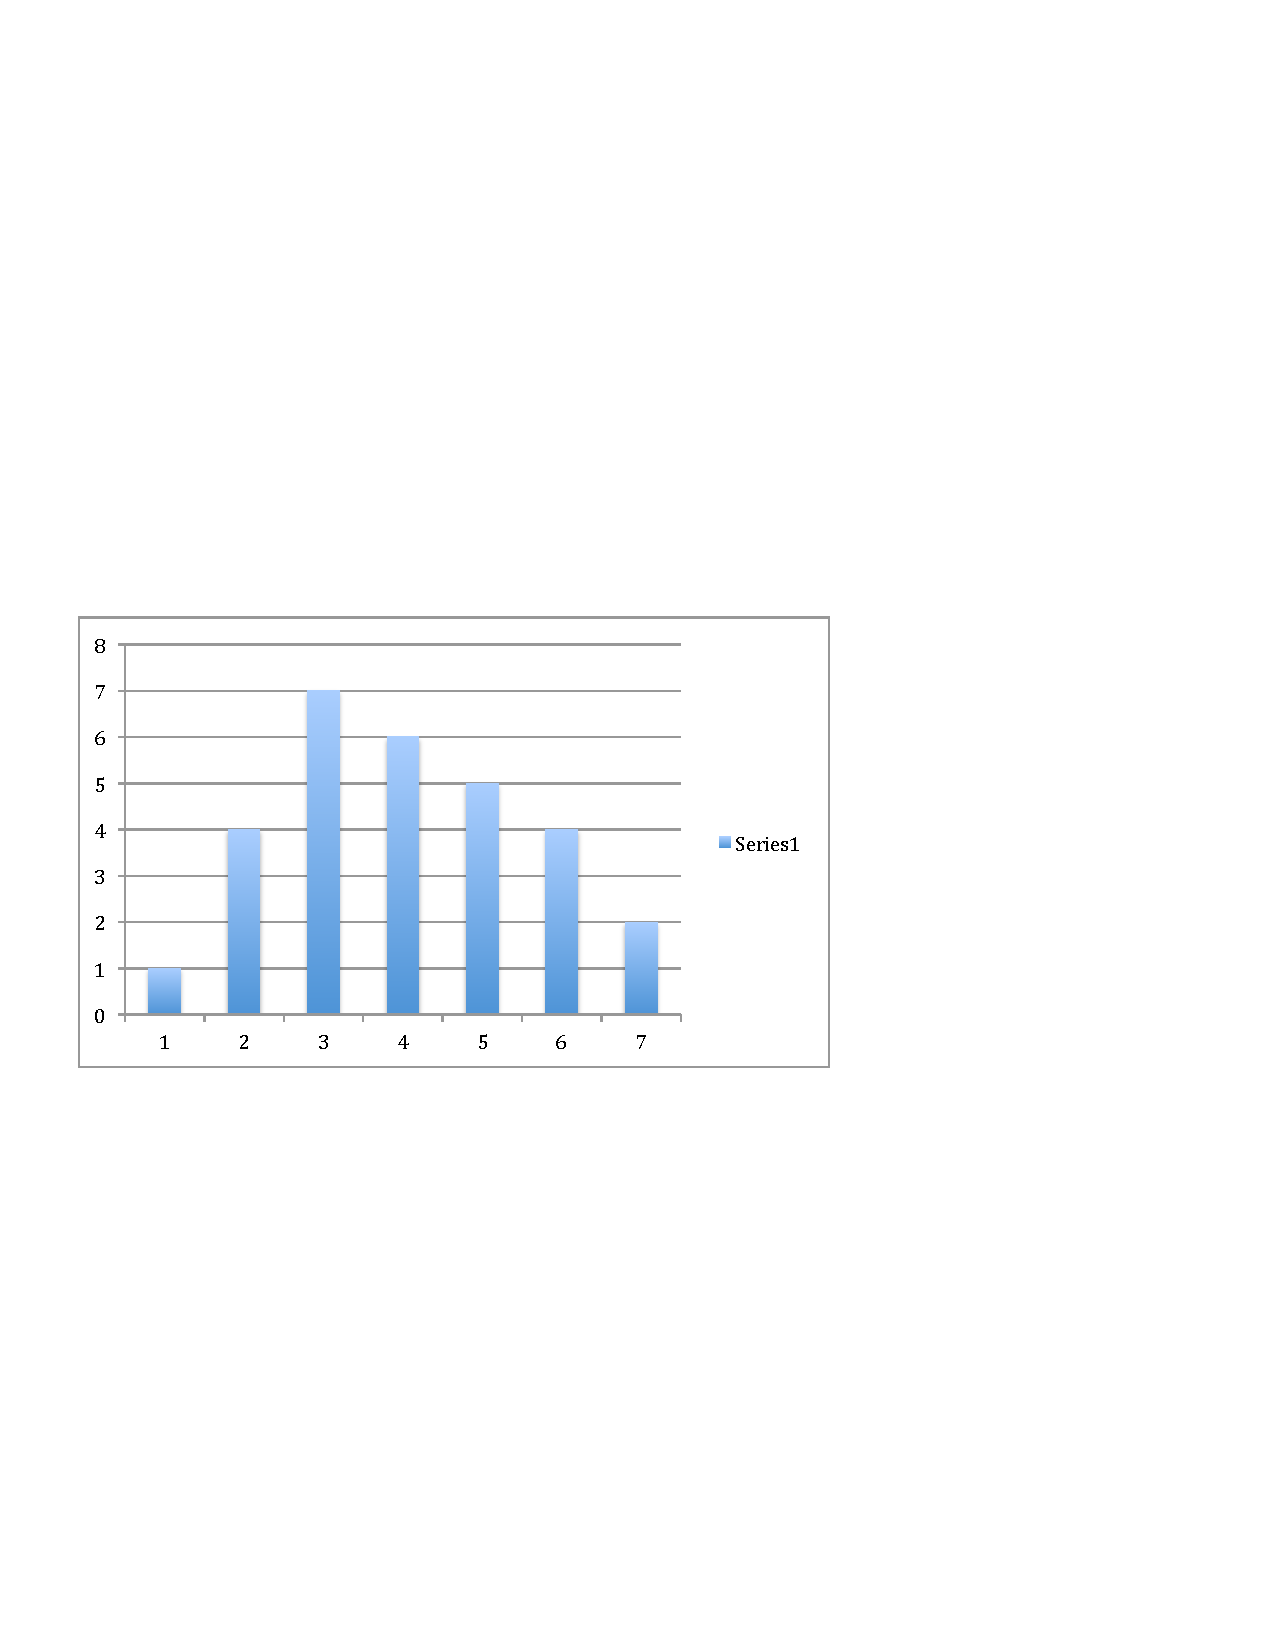
\includegraphics[width=.7\linewidth]{LabmanualFigures/Excel15.pdf}
      \caption{A figure for the histogram}
      \label{fig:excel15}
\end{figure}
 



\subsection{Paired Samples T-test} 
Suppose you ran an experiment with one independent variable that has 2 levels. You used a within- subject design so each participant contributed data to each of the 2 levels. You want to find out if there was significant effect. That is, is the mean performance in Level 1 different from mean performance in Level 2. An appropriate test is the paired-samples t-test.
Here is some sample data in Excel.
 and the number 1 tells excel to use a paired samples t-test. The resulting p-value is <.05 so we now know that there was a significant effect. The means for level 1 were significantly smaller than the means for level 2.

\begin{figure}
      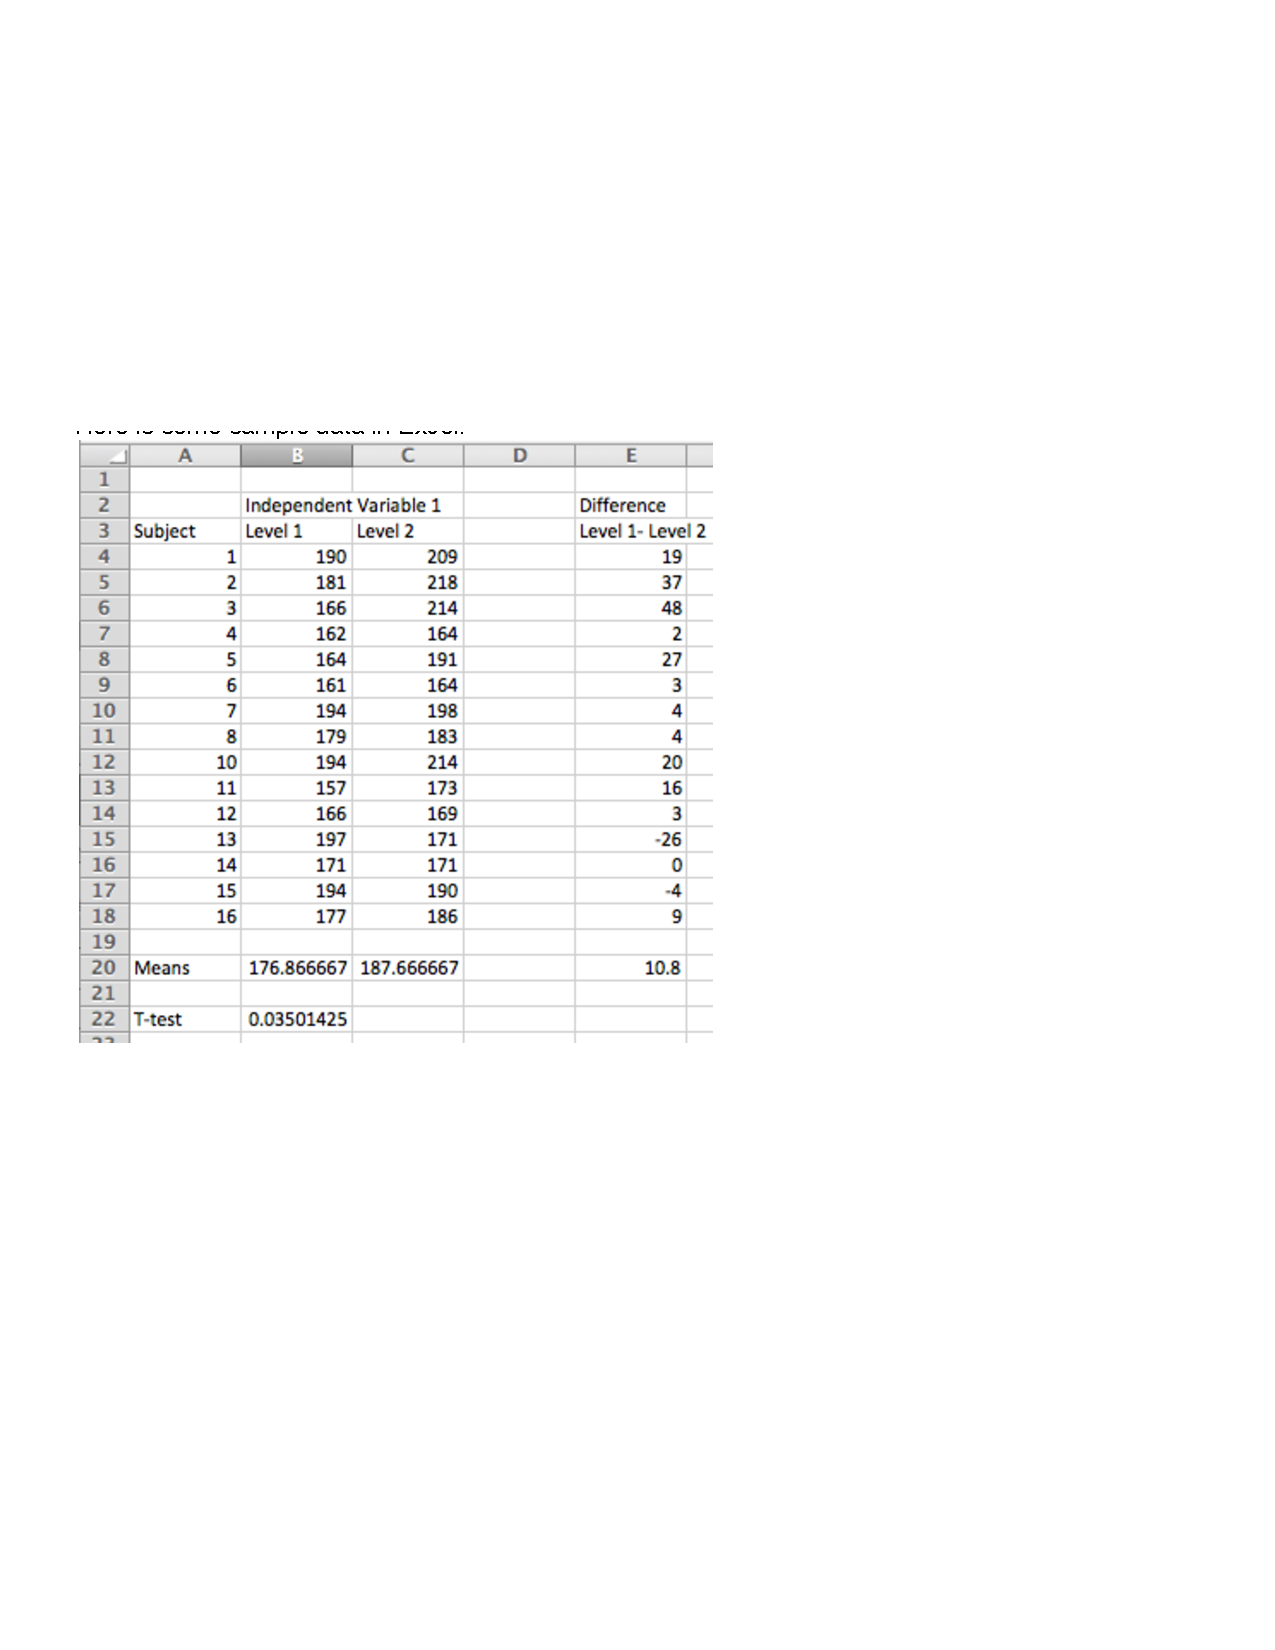
\includegraphics[width=.7\linewidth]{LabmanualFigures/Excel16.pdf}
      \caption{t test in excel}
      \label{fig:excel16}
\end{figure}
 


Tip: Even before you run a paired samples t-test you should have a good idea whether the test will be significant. You can get a ballpark estimate by computing the differences between means for each subject. This has been done in the example under the column labeled Difference. Here, the mean for level 1 has been subtracted from the mean for level 2 for each subject. This gives us a difference score. Look at all of the difference scores. You will see that almost all of them (except for 2) are positive. So, most of the subjects showed the effect. As a ballpark rule, when most of the subjects show the effect you should expect that a t-test will likely show a significant result.

\section{SPSS}

\subsection{Paired Samples T-test in SPSS} 

\begin{figure}
      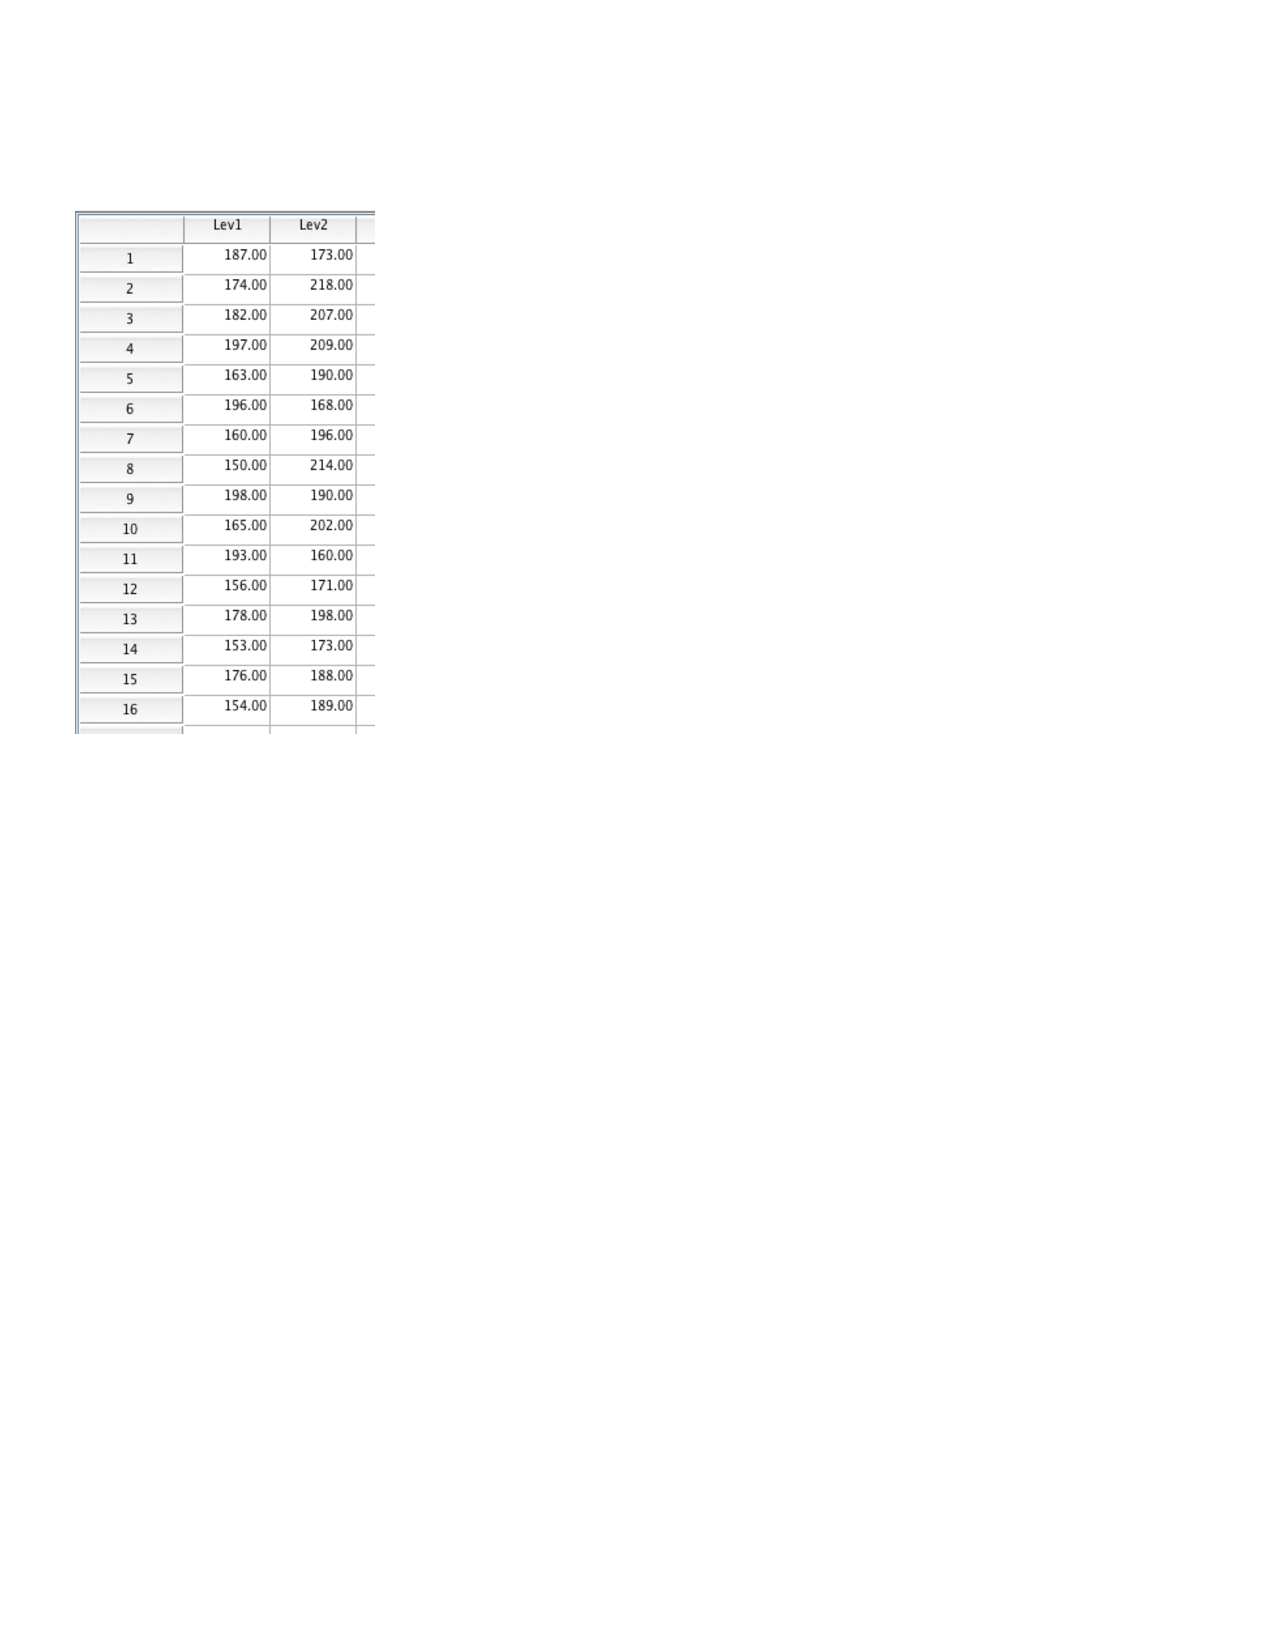
\includegraphics[width=.5\linewidth]{LabmanualFigures/SPSS1.pdf}
      \caption{Copy the data into SPSS}
      \label{fig:spss1}
\end{figure}

1. Copy the data for each level of the independent variable into separate columns in the data editor. In the example I've given new names (lev1, lev2) to each of the conditions.


\begin{figure}
      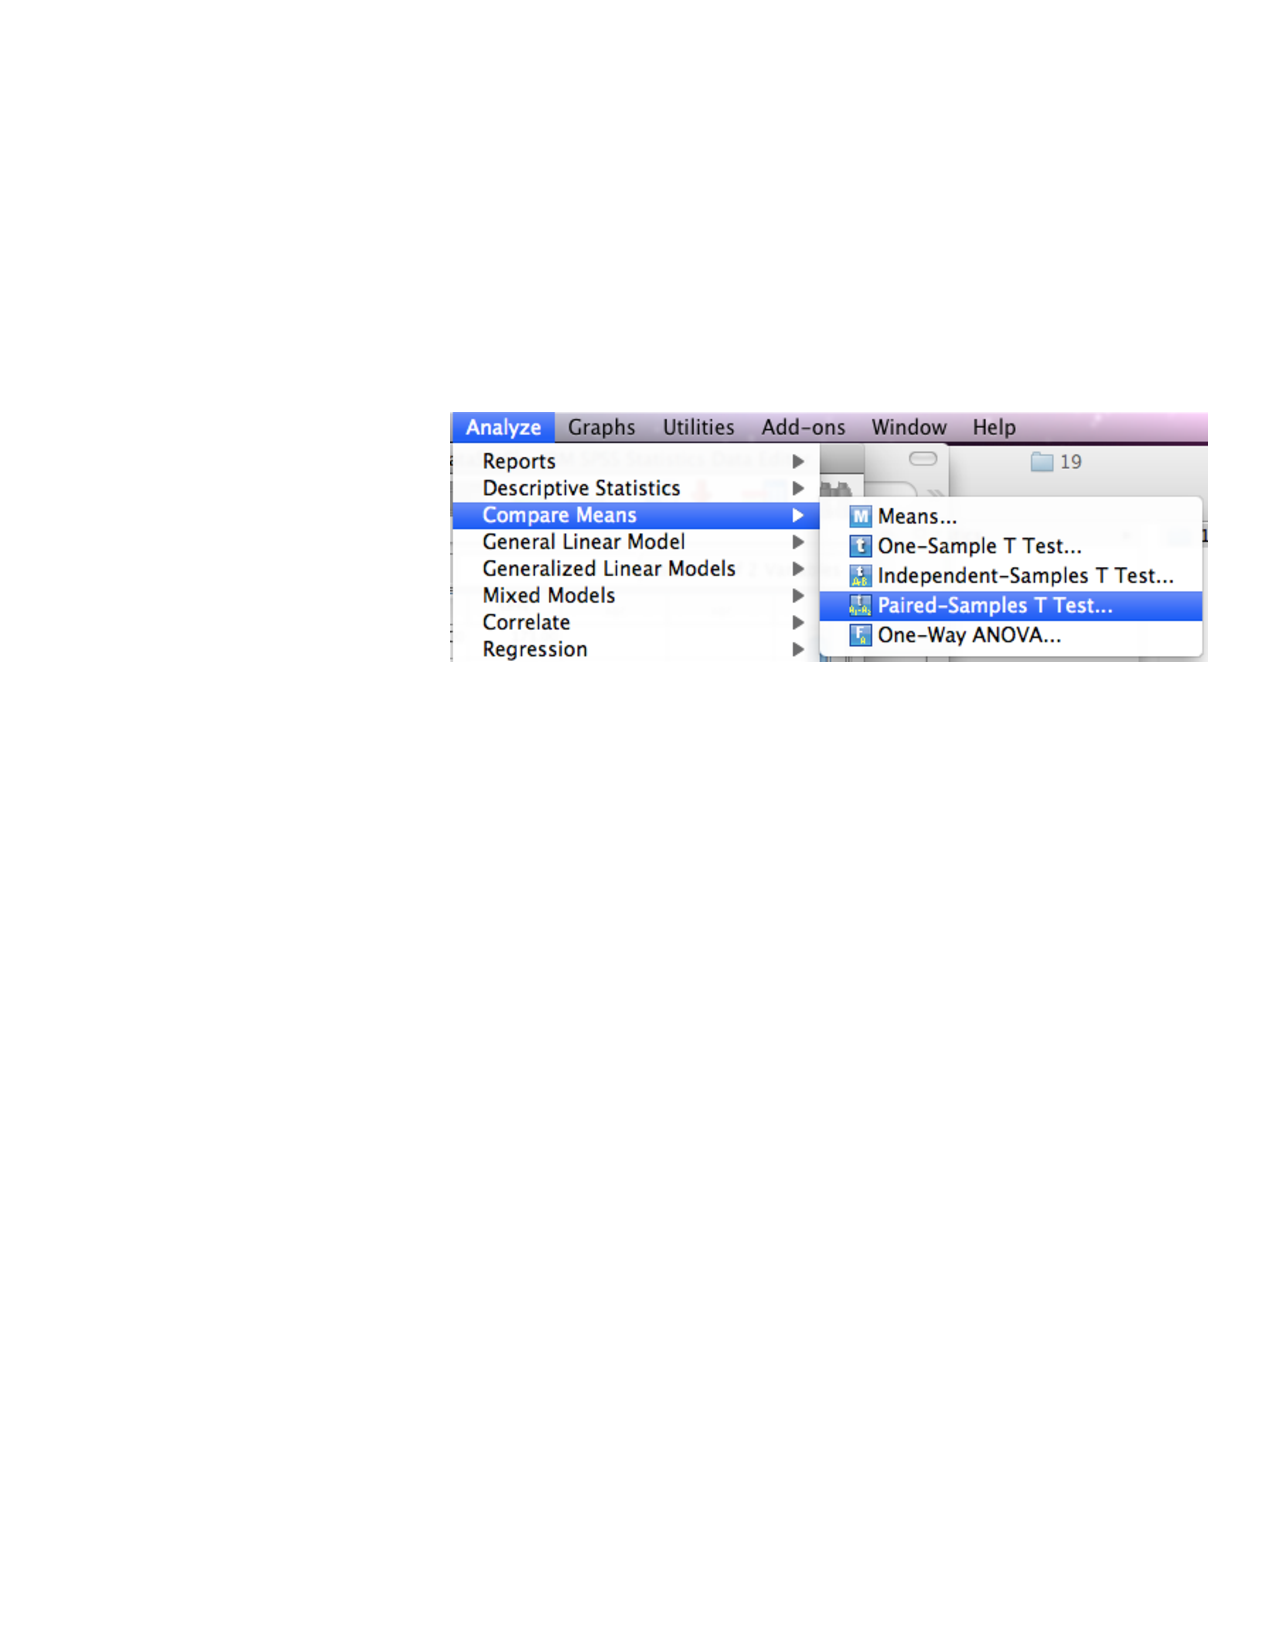
\includegraphics[width=.5\linewidth]{LabmanualFigures/SPSS2.pdf}
      \caption{Choose t-test}
      \label{fig:SPSS2}
\end{figure}

2. Next,choose analyze from the menu, select Compare Means, then select Paired-Samples T Test


3. You will see the following menu. Select both of your variables (Lev1, Lev2) then press the arrow button to move them into the paired variables list
   

\begin{figure}
      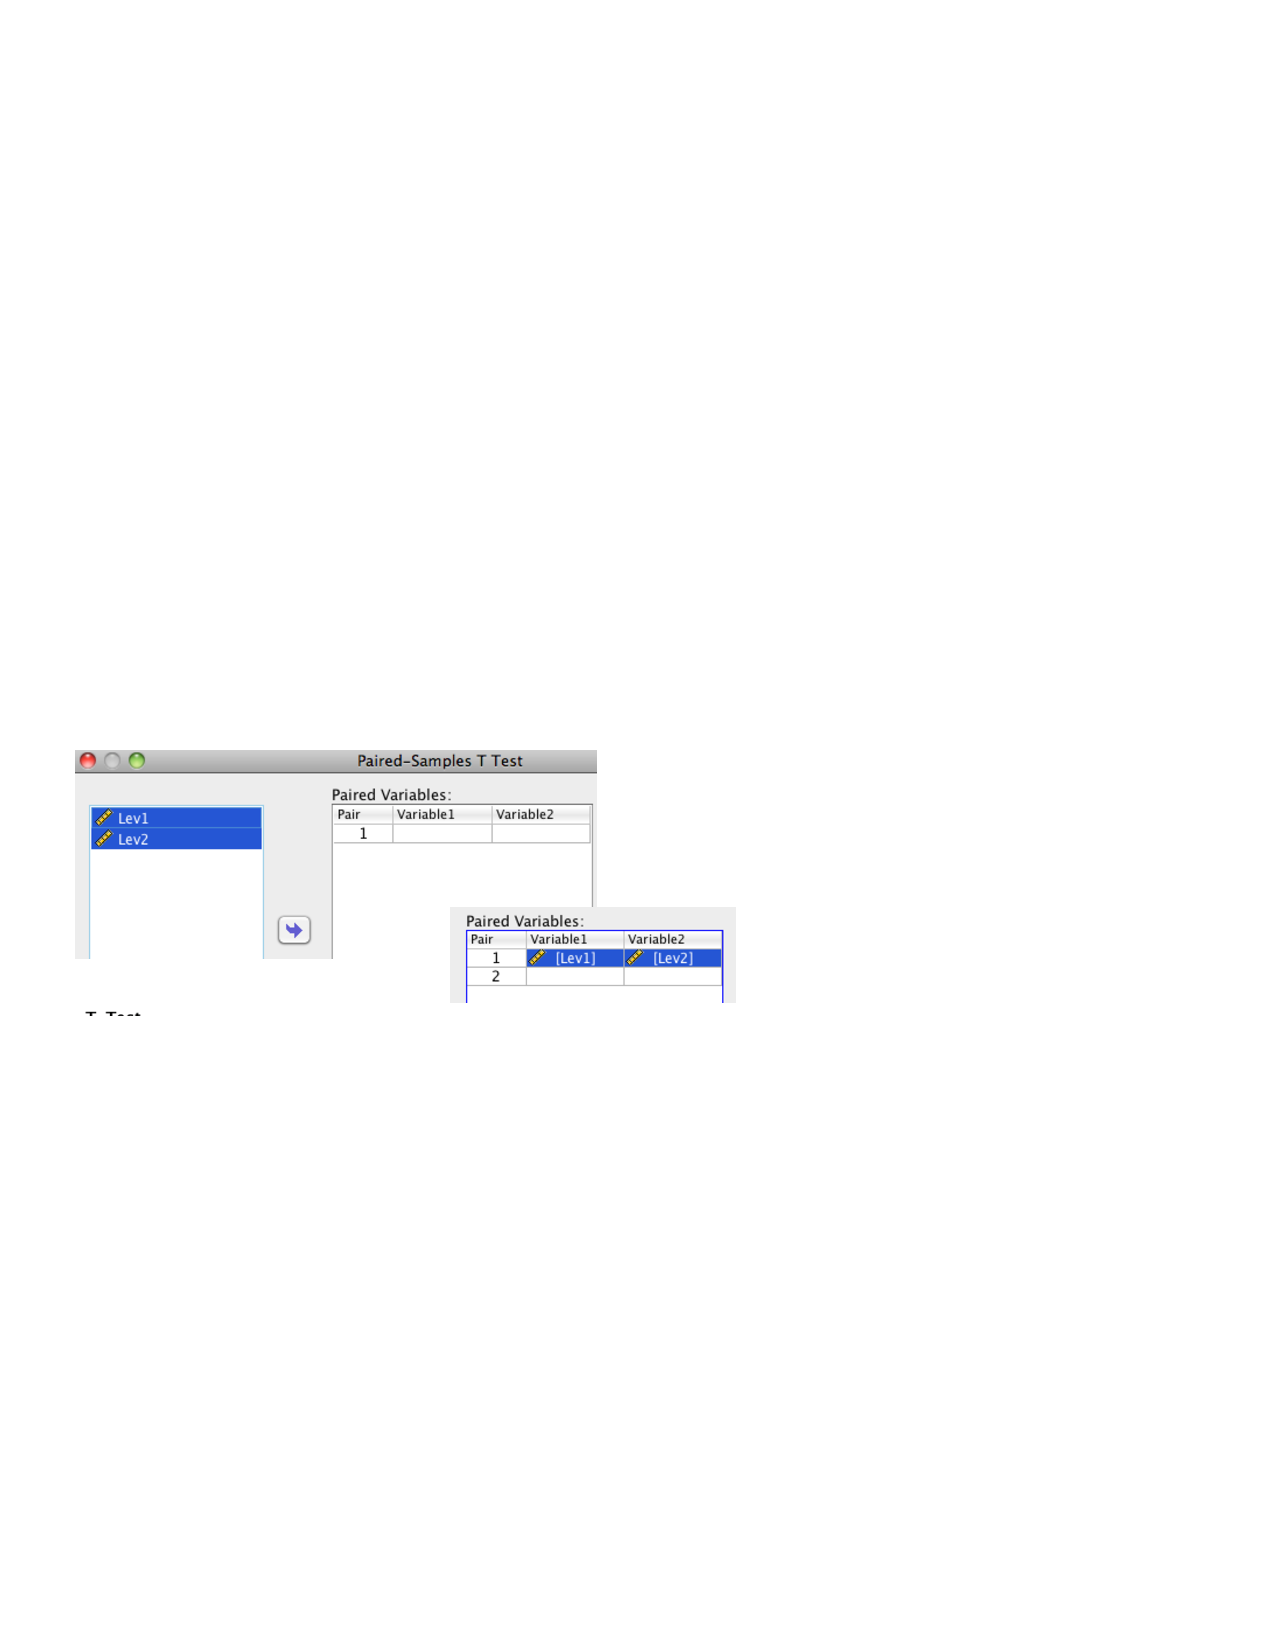
\includegraphics[width=.5\linewidth]{LabmanualFigures/SPSS3.pdf}
      \caption{Select levels}
      \label{fig:SPSS3}
\end{figure}

4. It should look like this... now click the button for the analysis


5. The first box shows basic descriptive statistics, means, number per cell, standard deviation and standard error of the mean.


\begin{figure}
      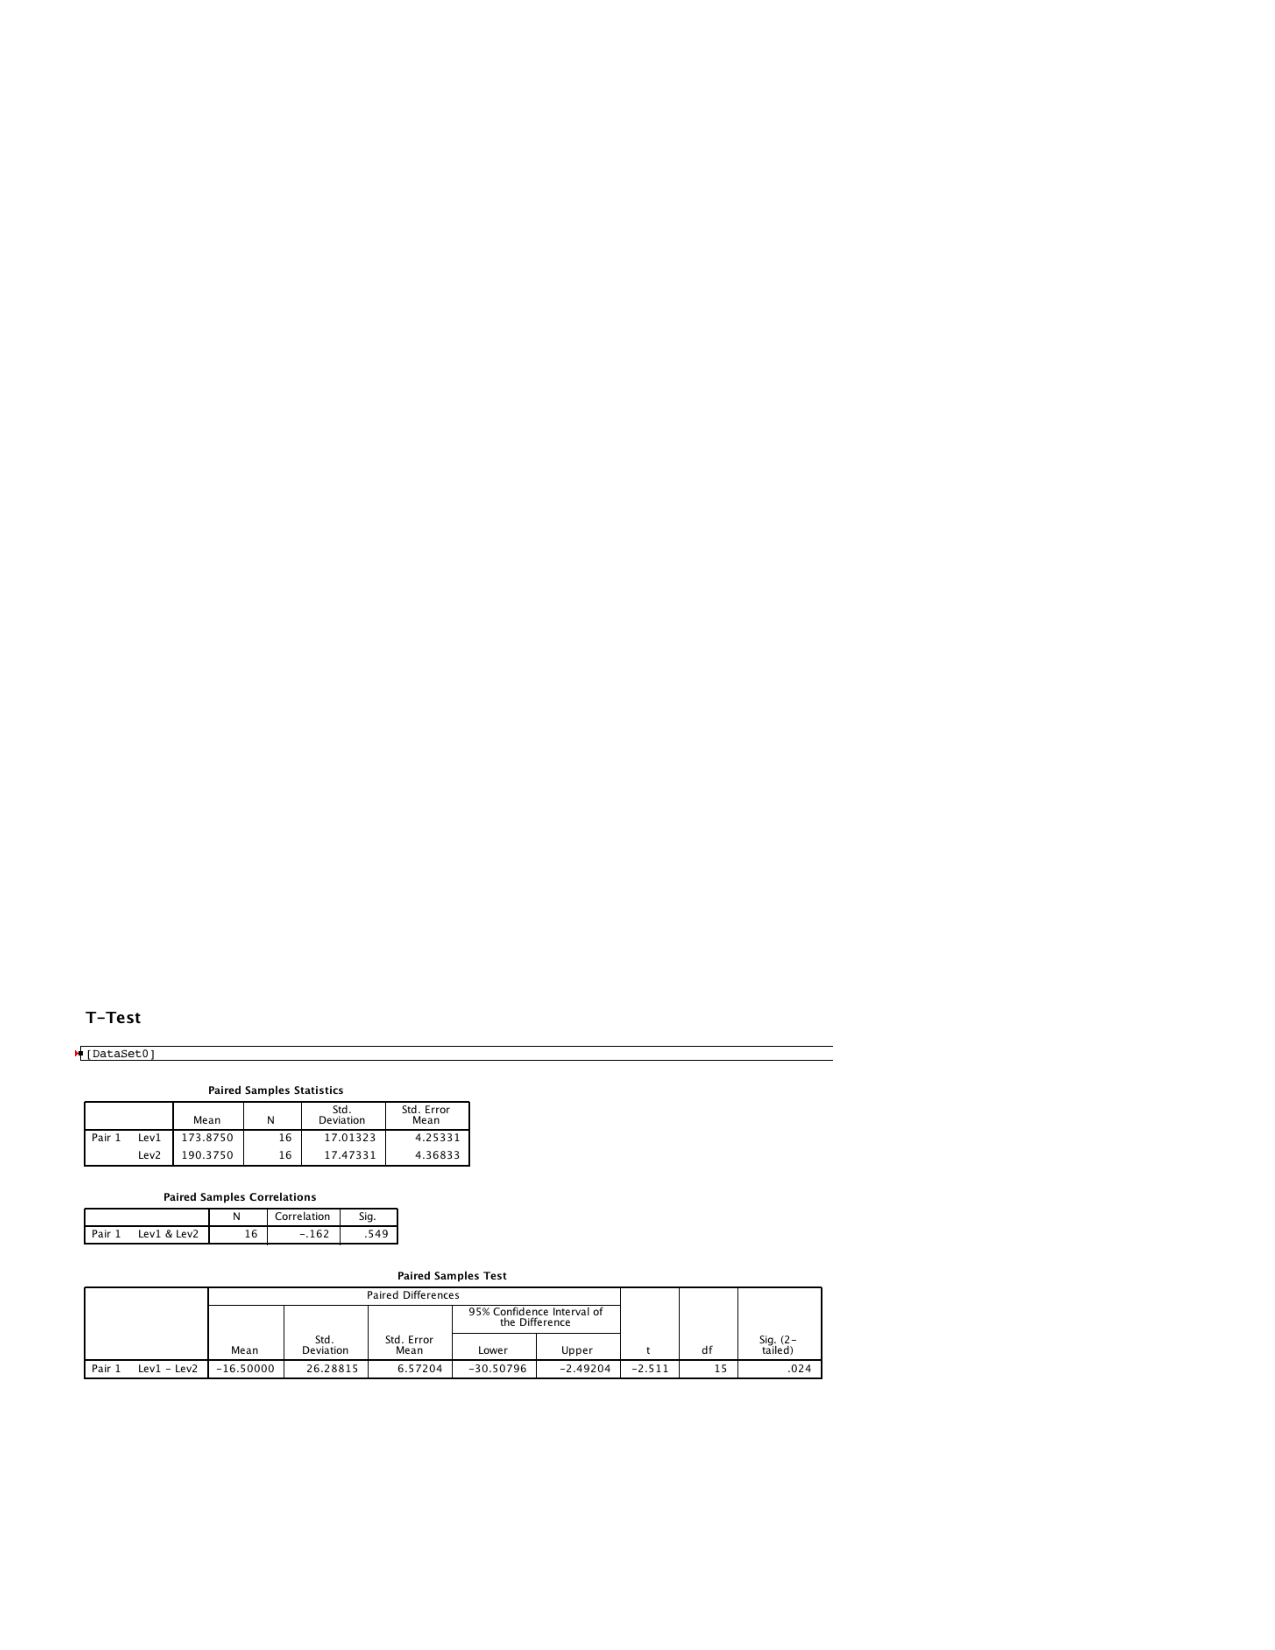
\includegraphics[width=\linewidth]{LabmanualFigures/SPSS4.pdf}
      \caption{ttest output}
      \label{fig:SPSS4}
\end{figure}

6. The third box shows the t-value, the associated degrees of freedom (df), and the p- value (Sig. (2-tailed)


7. Here's how you write up your results in one sentence.


8. Means were significantly smaller for level 1 (174) than level 2 (190), t(15) = 2.51, p<.05.
  
\subsection{2 x 2 Repeated Measures ANOVA}
\subsection{From Data to Analysis}

Suppose you ran an experiment with 2 independent variables, each with 2 levels. If this is a within- subject design, each participant will contribute data to each of the 4 levels in the design. The appropriate test is a 2x2 repeated measures ANOVA. We begin by looking at the data in excel.


\begin{figure}
      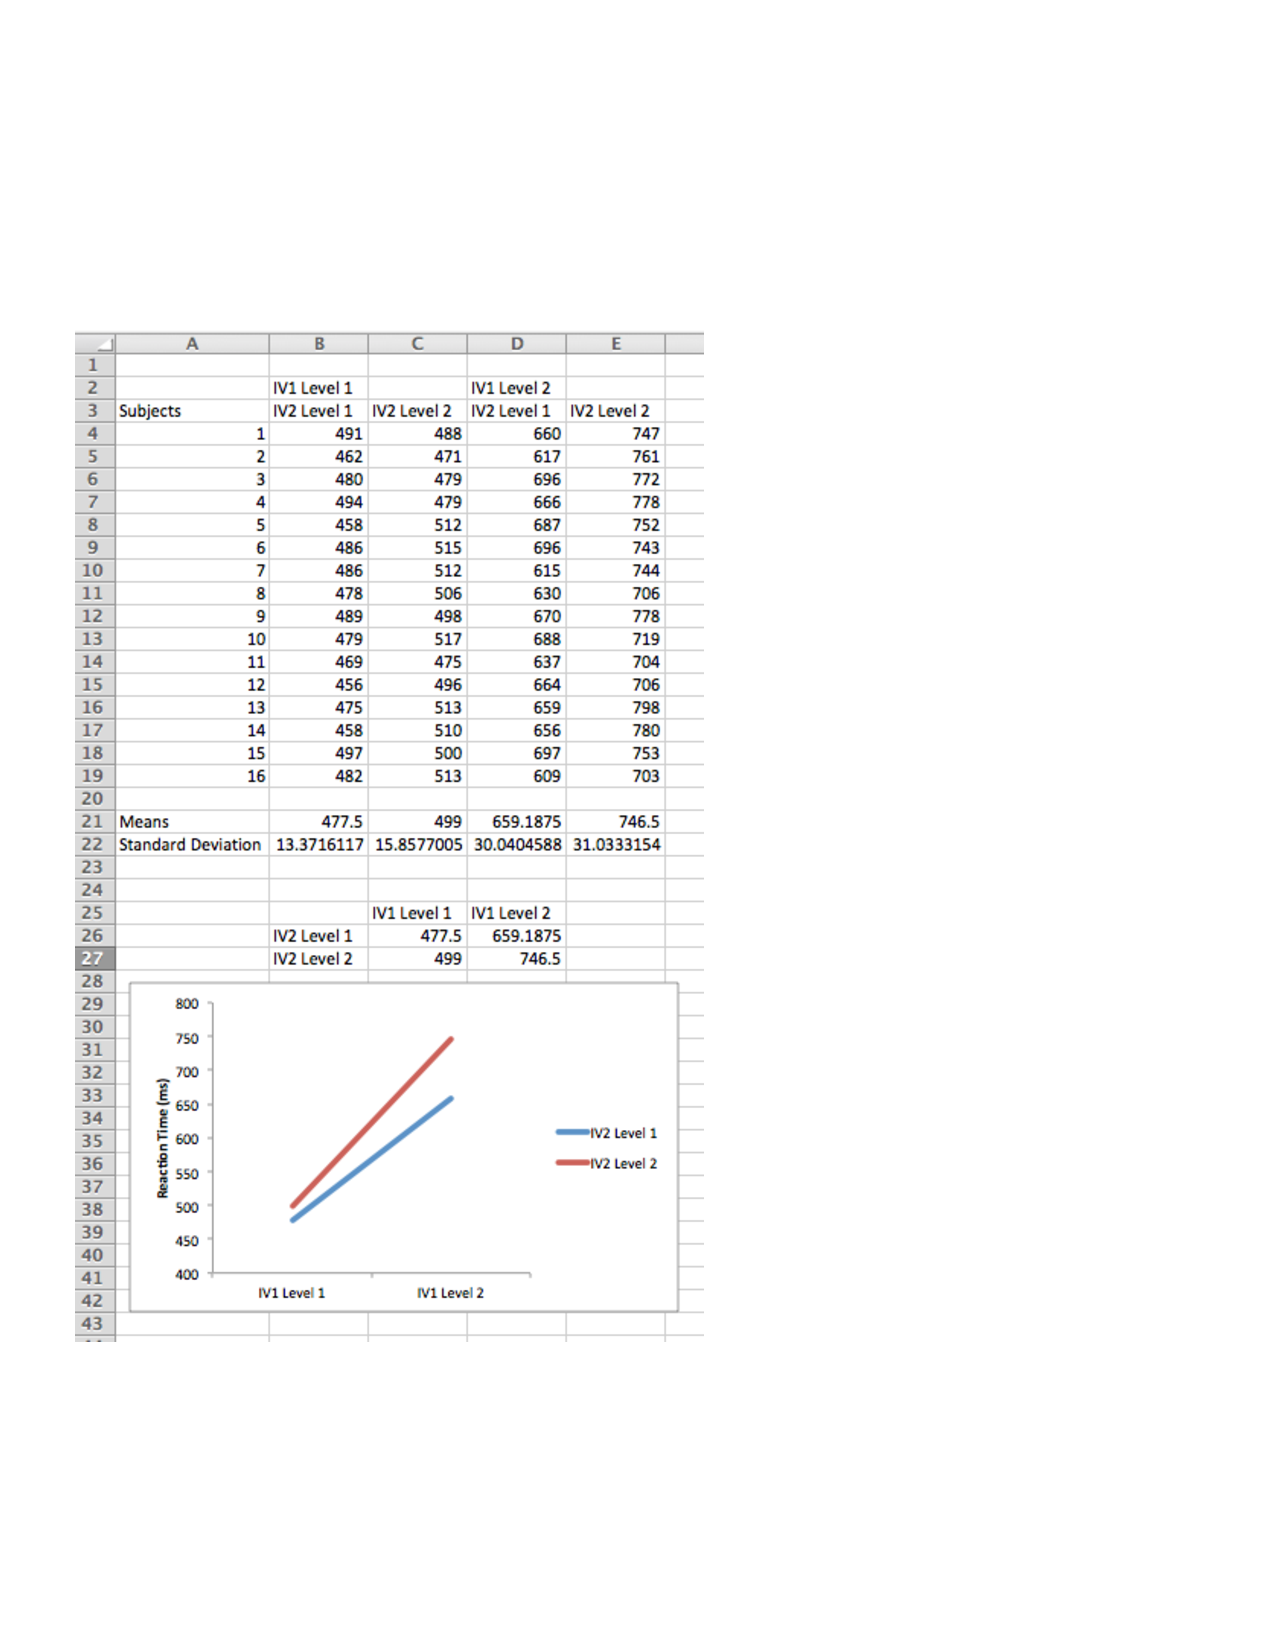
\includegraphics[width=.7\linewidth]{LabmanualFigures/SPSS5.pdf}
      \caption{Sample data for a 2 x 2 factorial design}
      \label{fig:SPSS5}
\end{figure}

1. All of the four conditions are placed into 4 separate columns. The second IV is nested underneath the first IV.

2. The means and standard deviations can be computed directly in excel for each of the conditions

3. The means are then organized in a table, and a figure can be created so that we can see the pattern of results.

4. Main effects: It looks like there are two main effects. One for IV1: level 1 is smaller than level 2. One for IV2: level 1 is smaller than level 2

5. Interaction:It looks like there is an interaction. The difference between L1 and L2 of IV1 is larger for level 1 of IV2 (in red) than level 2 of IV2 (in blue).

6. We need to run a 2x2 repeated
measures ANOVA to determine whether the main effects are significant, and to determine if the interaction is significant.


\subsection{2x2 Repeated measures ANOVA in SPSS}
 
\begin{figure}
      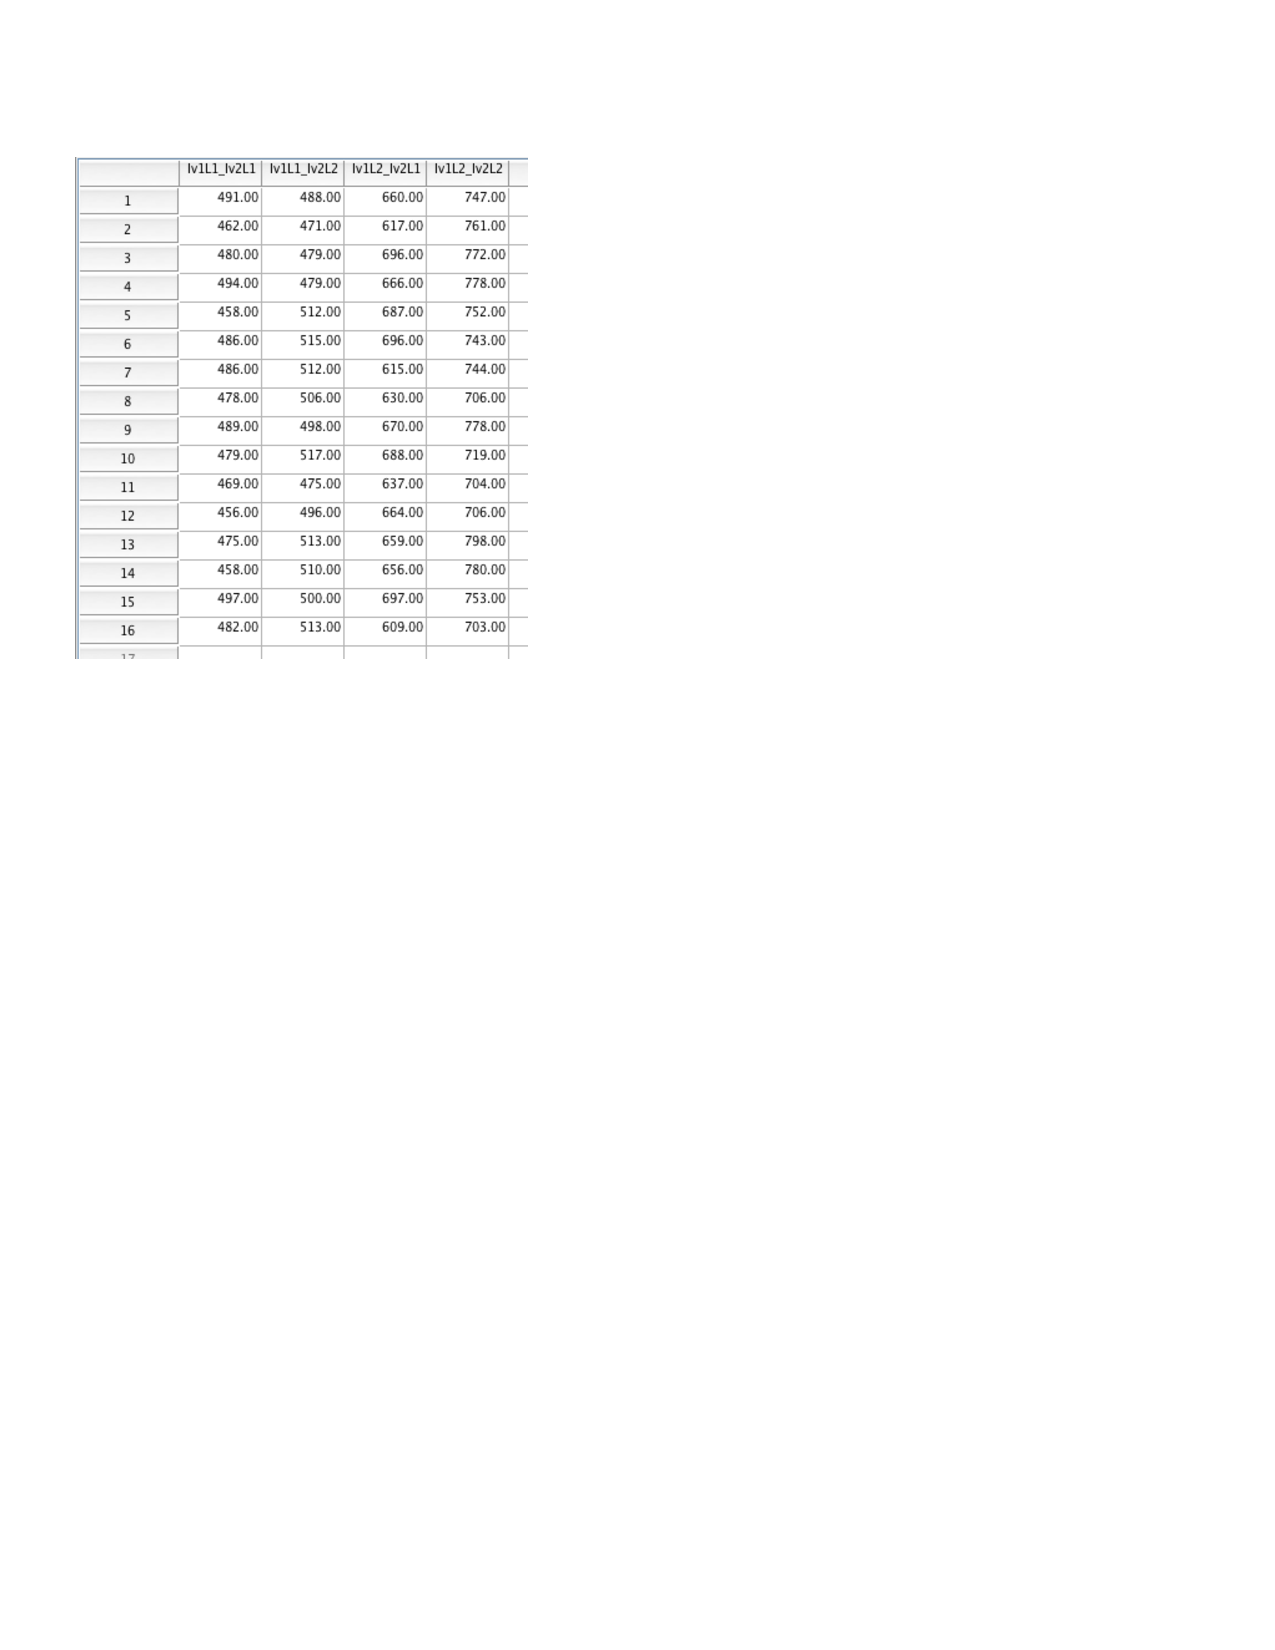
\includegraphics[width=.6\linewidth]{LabmanualFigures/SPSS6.pdf}
      \caption{Copy data into SPSS}
      \label{fig:SPSS6}
\end{figure}

1. Copy the data into SPSS. Make sure each column represents a different condition in the design.

2. Give names to each of the variables. The first column represents IV1 Level1 \& IV2 Level 1. The second column represents IV1 Level 1 \& IV2 Level 2. The third column represents IV1 Level 2 \& IV2 Level 1. The fourth column represents IV1 Level 2 \& IV2 Level 2.

\begin{figure}
      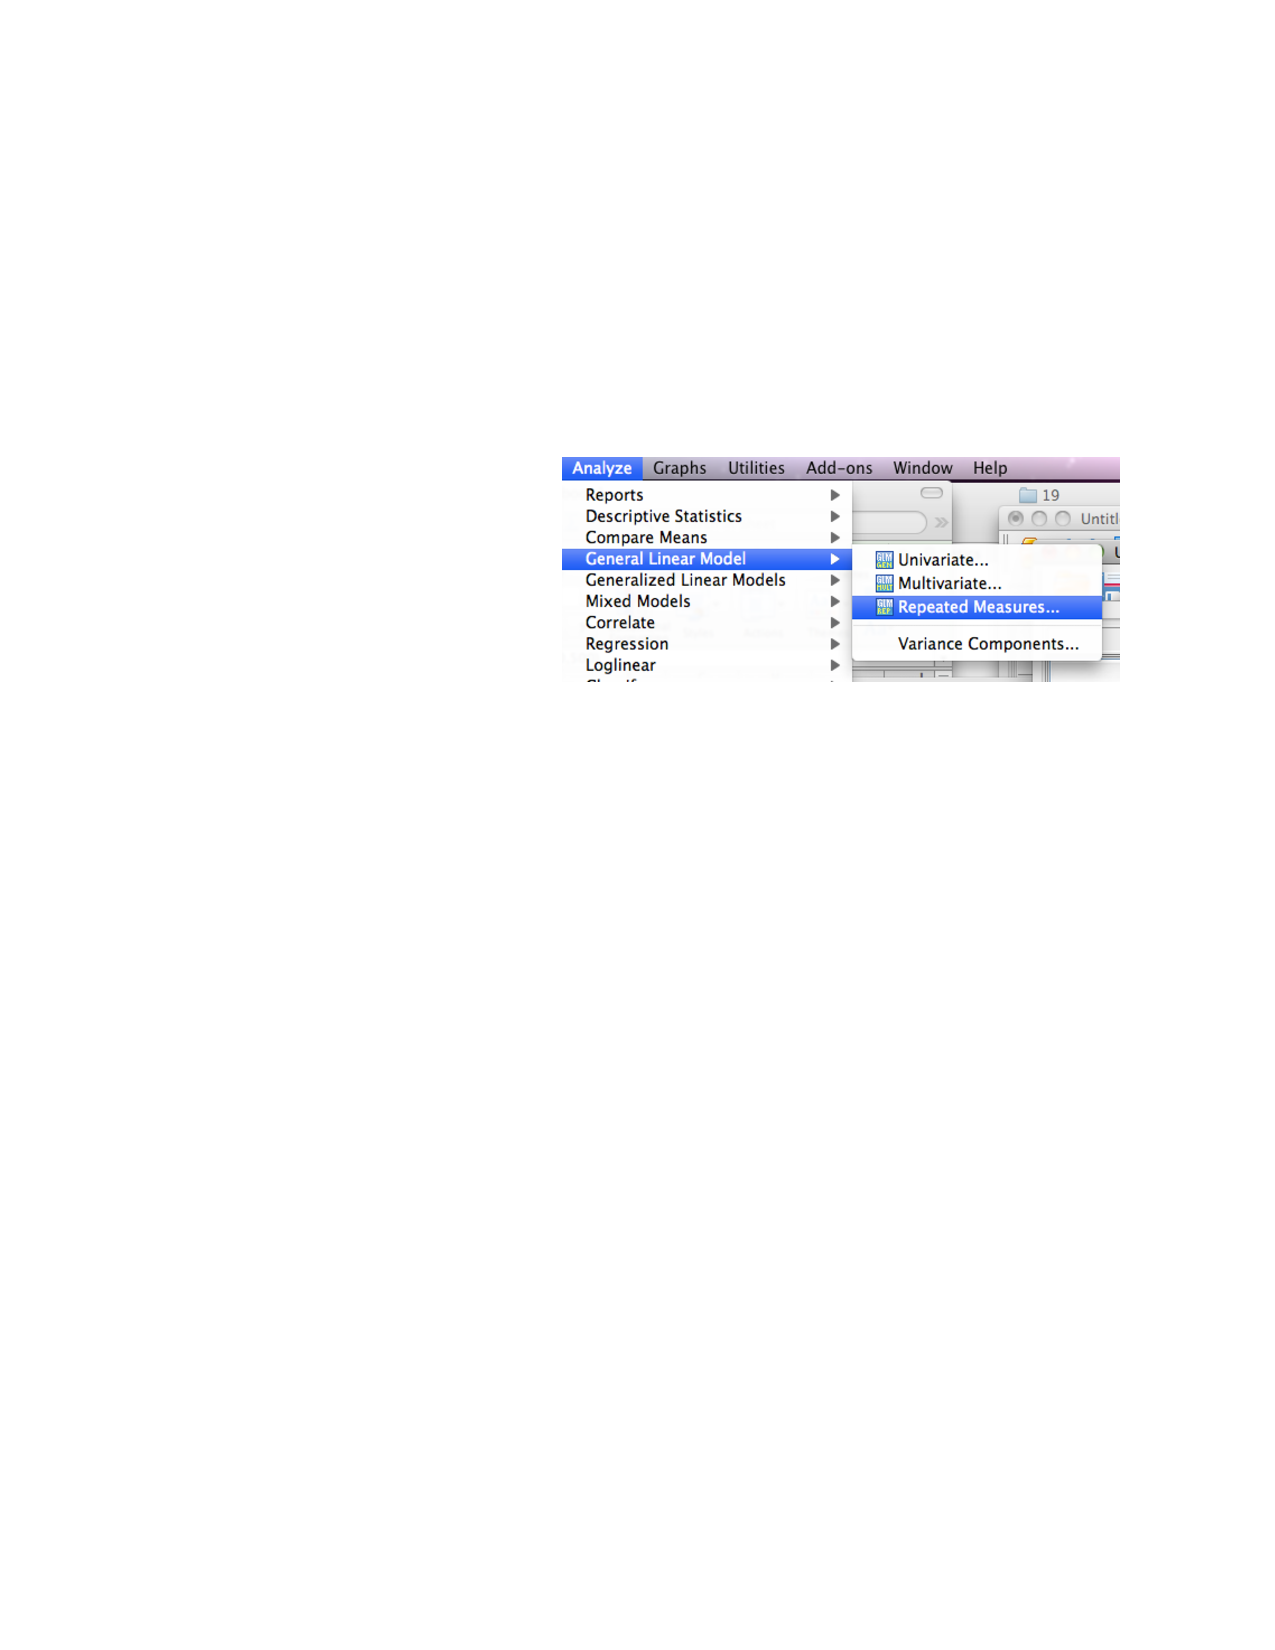
\includegraphics[width=.5\linewidth]{LabmanualFigures/SPSS7.pdf}
      \caption{Choose the model}
 	\label{fig:sp7}
\end{figure}

3. Choose Analyze, General Linear Model, Repeated Measures from the menu.
   
\begin{figure}
      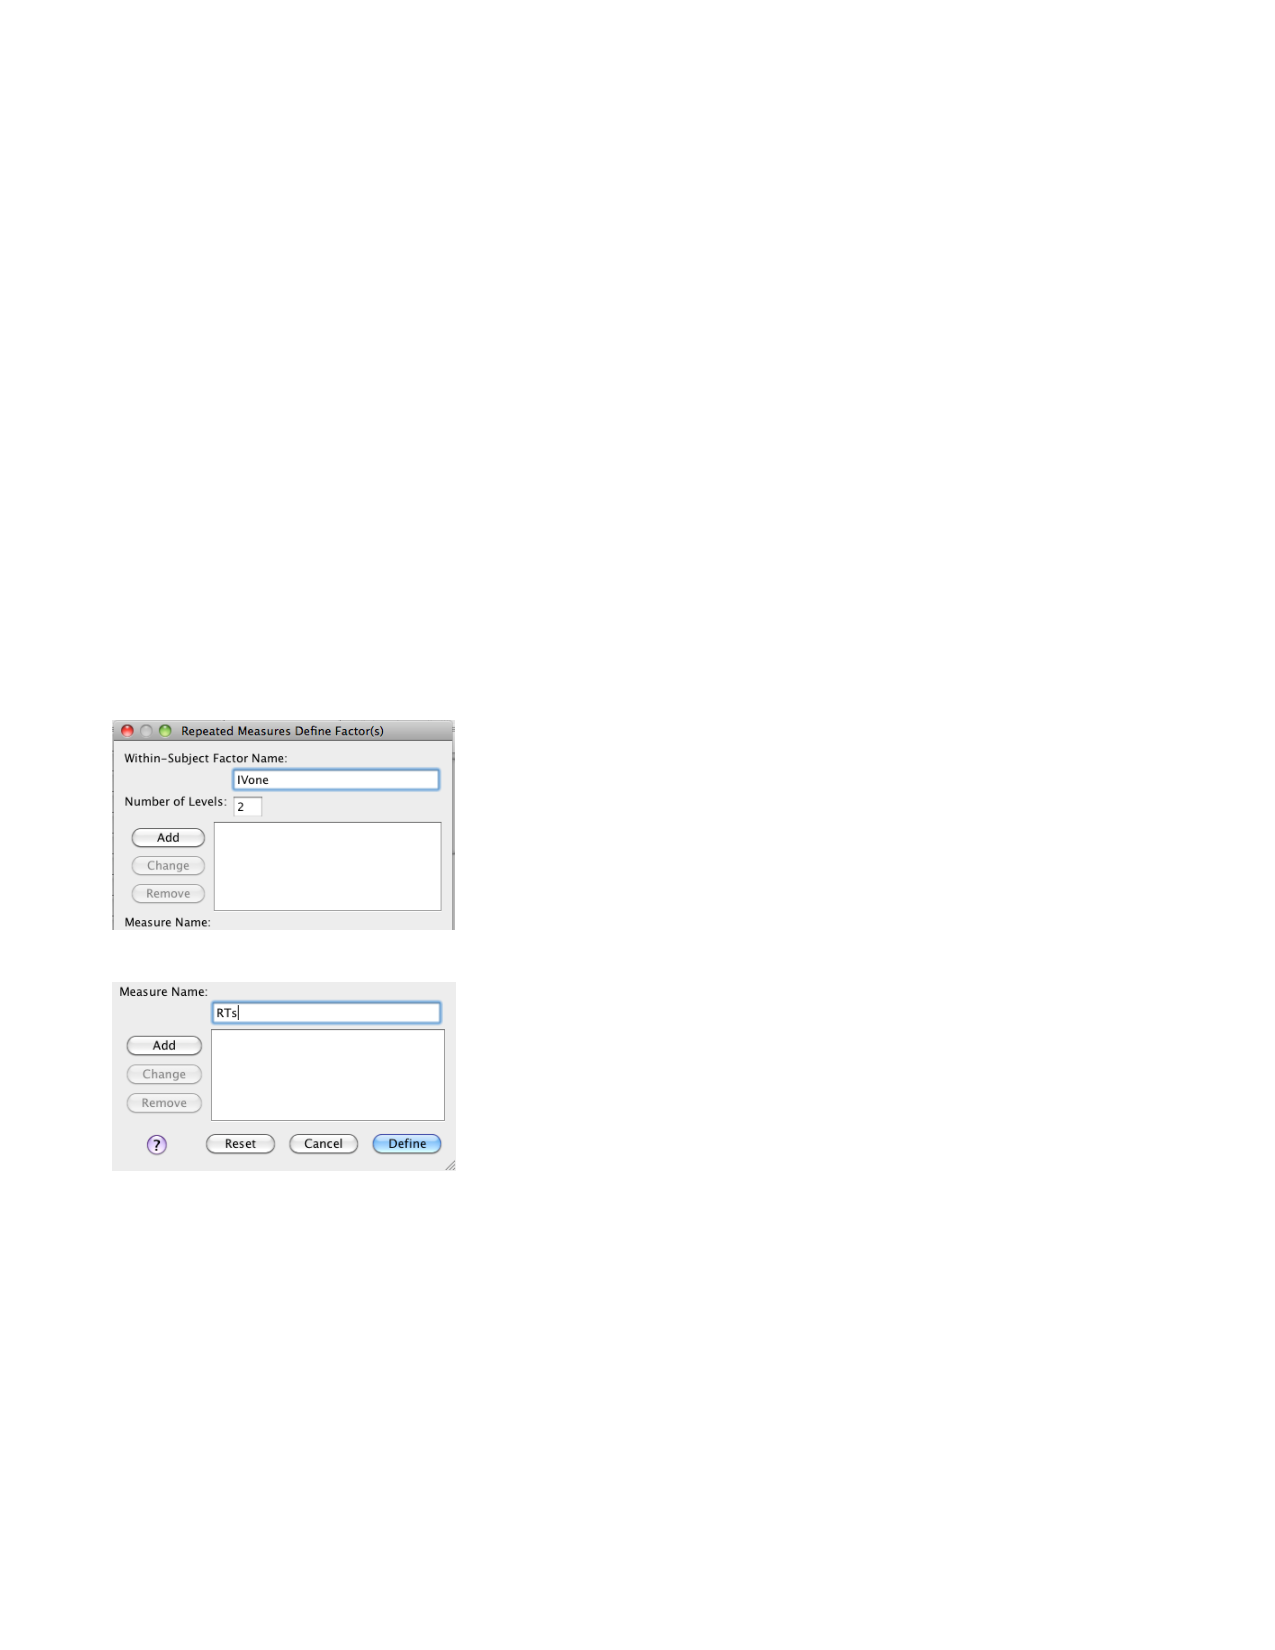
\includegraphics[width=.5\linewidth]{LabmanualFigures/SPSS8.pdf}
      \caption{Name variables}
      \label{fig:SPSS8}
\end{figure}

\begin{figure}
      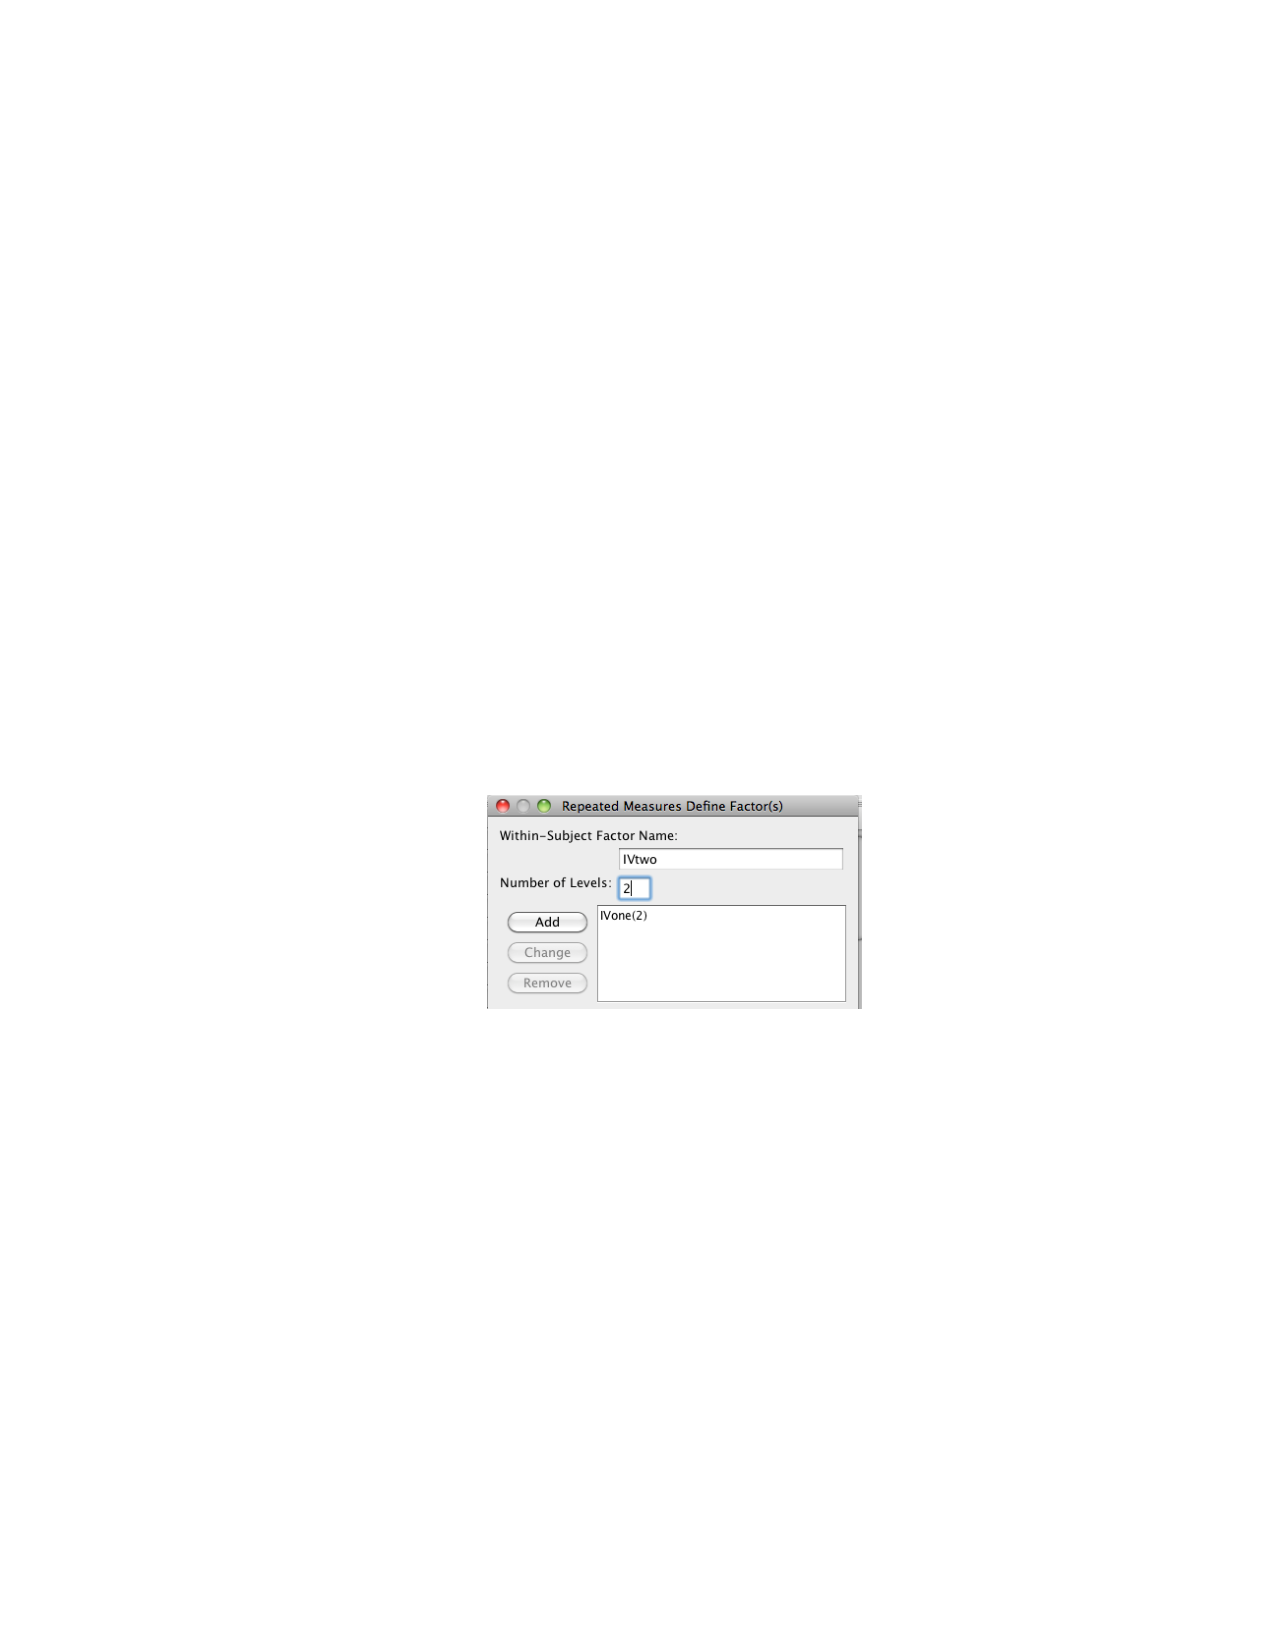
\includegraphics[width=.5\linewidth]{LabmanualFigures/SPSS9.pdf}
      \caption{ thing a}
      \label{fig:SPSS9}
\end{figure}

4. Name IV1, specify 2 levels

5. Name IV1, specify 2 levels

6. Name dependent variable, click define

7. Select all four conditions, press the first right arrow, if you want more options see below, otherwise press ok.

\begin{figure}
      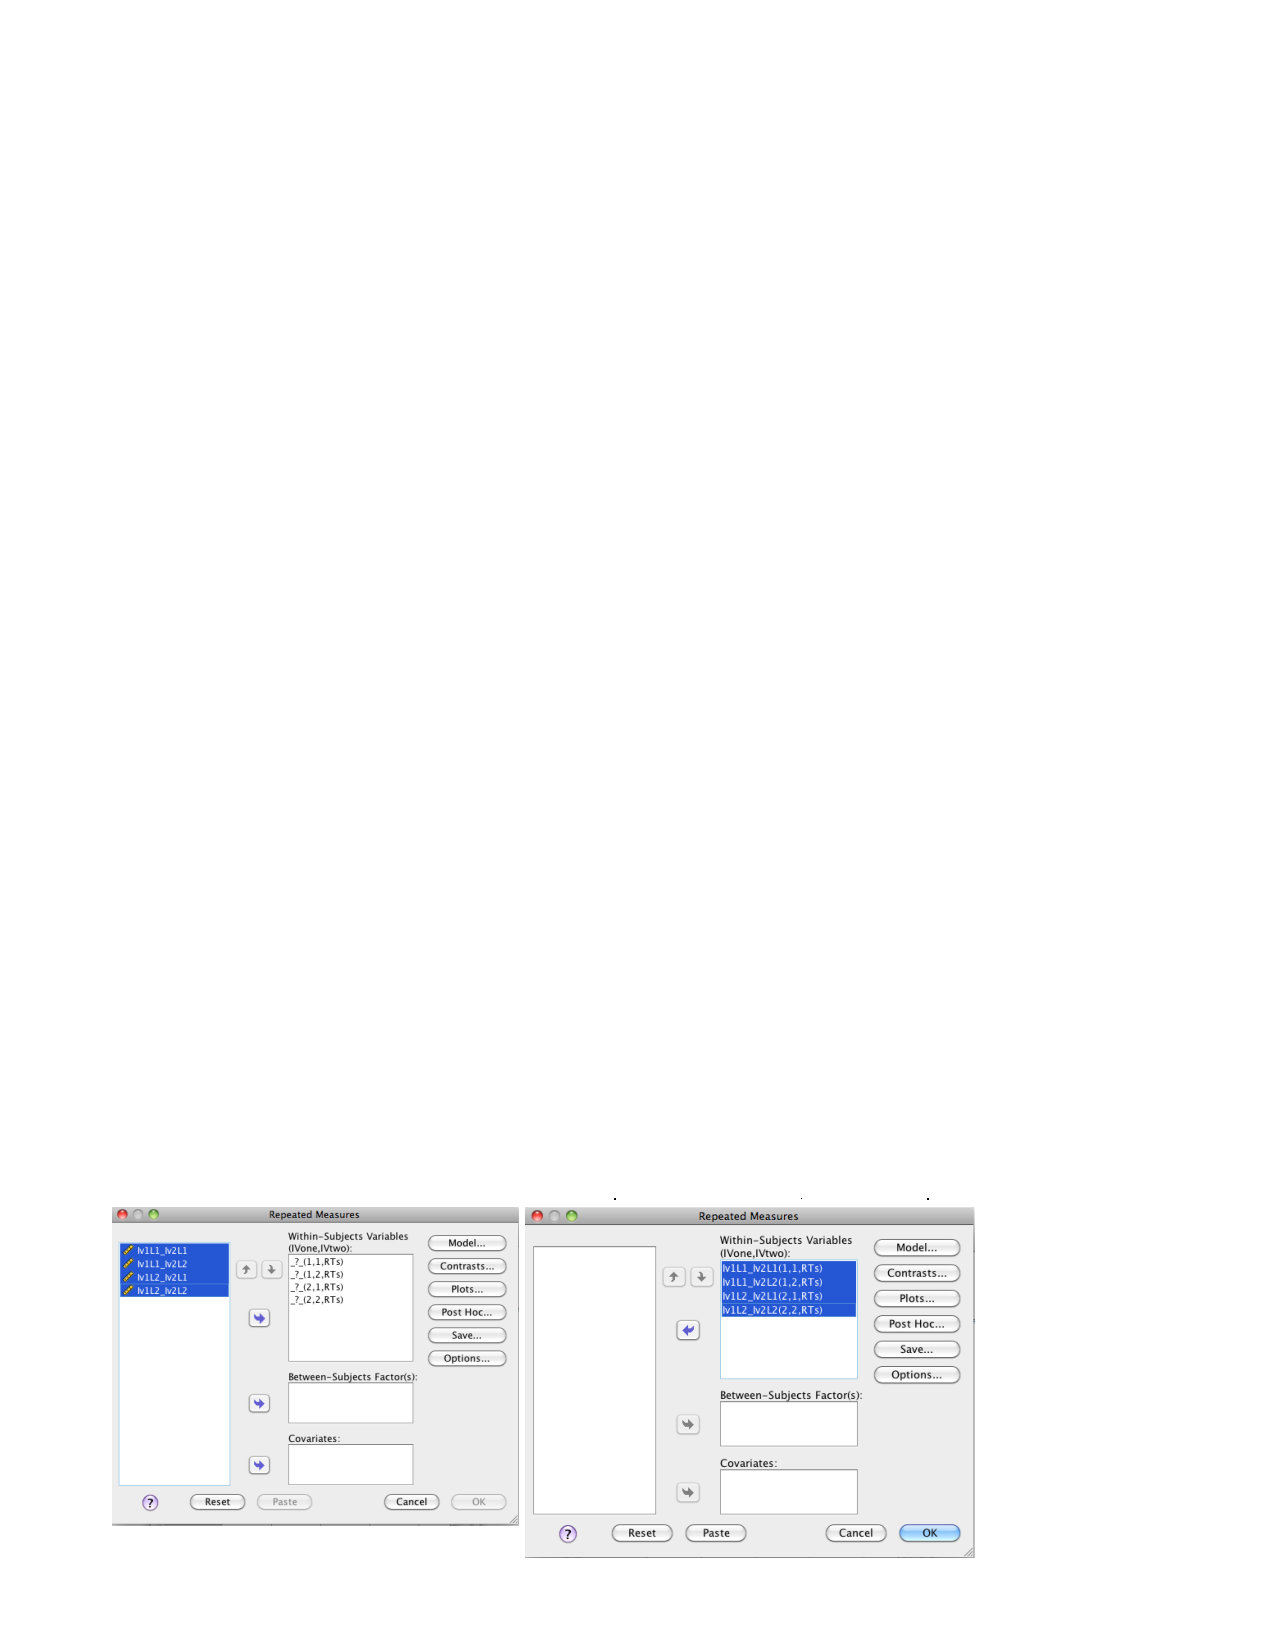
\includegraphics[width=\linewidth]{LabmanualFigures/SPSS10.pdf}
      \caption{Select conditions}
      \label{fig:SPSS10}
\end{figure}

8. If you pressed options, then you can ask SPSS to report descriptive statistics for each condition. Choose the factors that you want, then press the arrow button to move them into the display means field. Make sure you click descriptive statistics. Then click continue.

\begin{figure}
      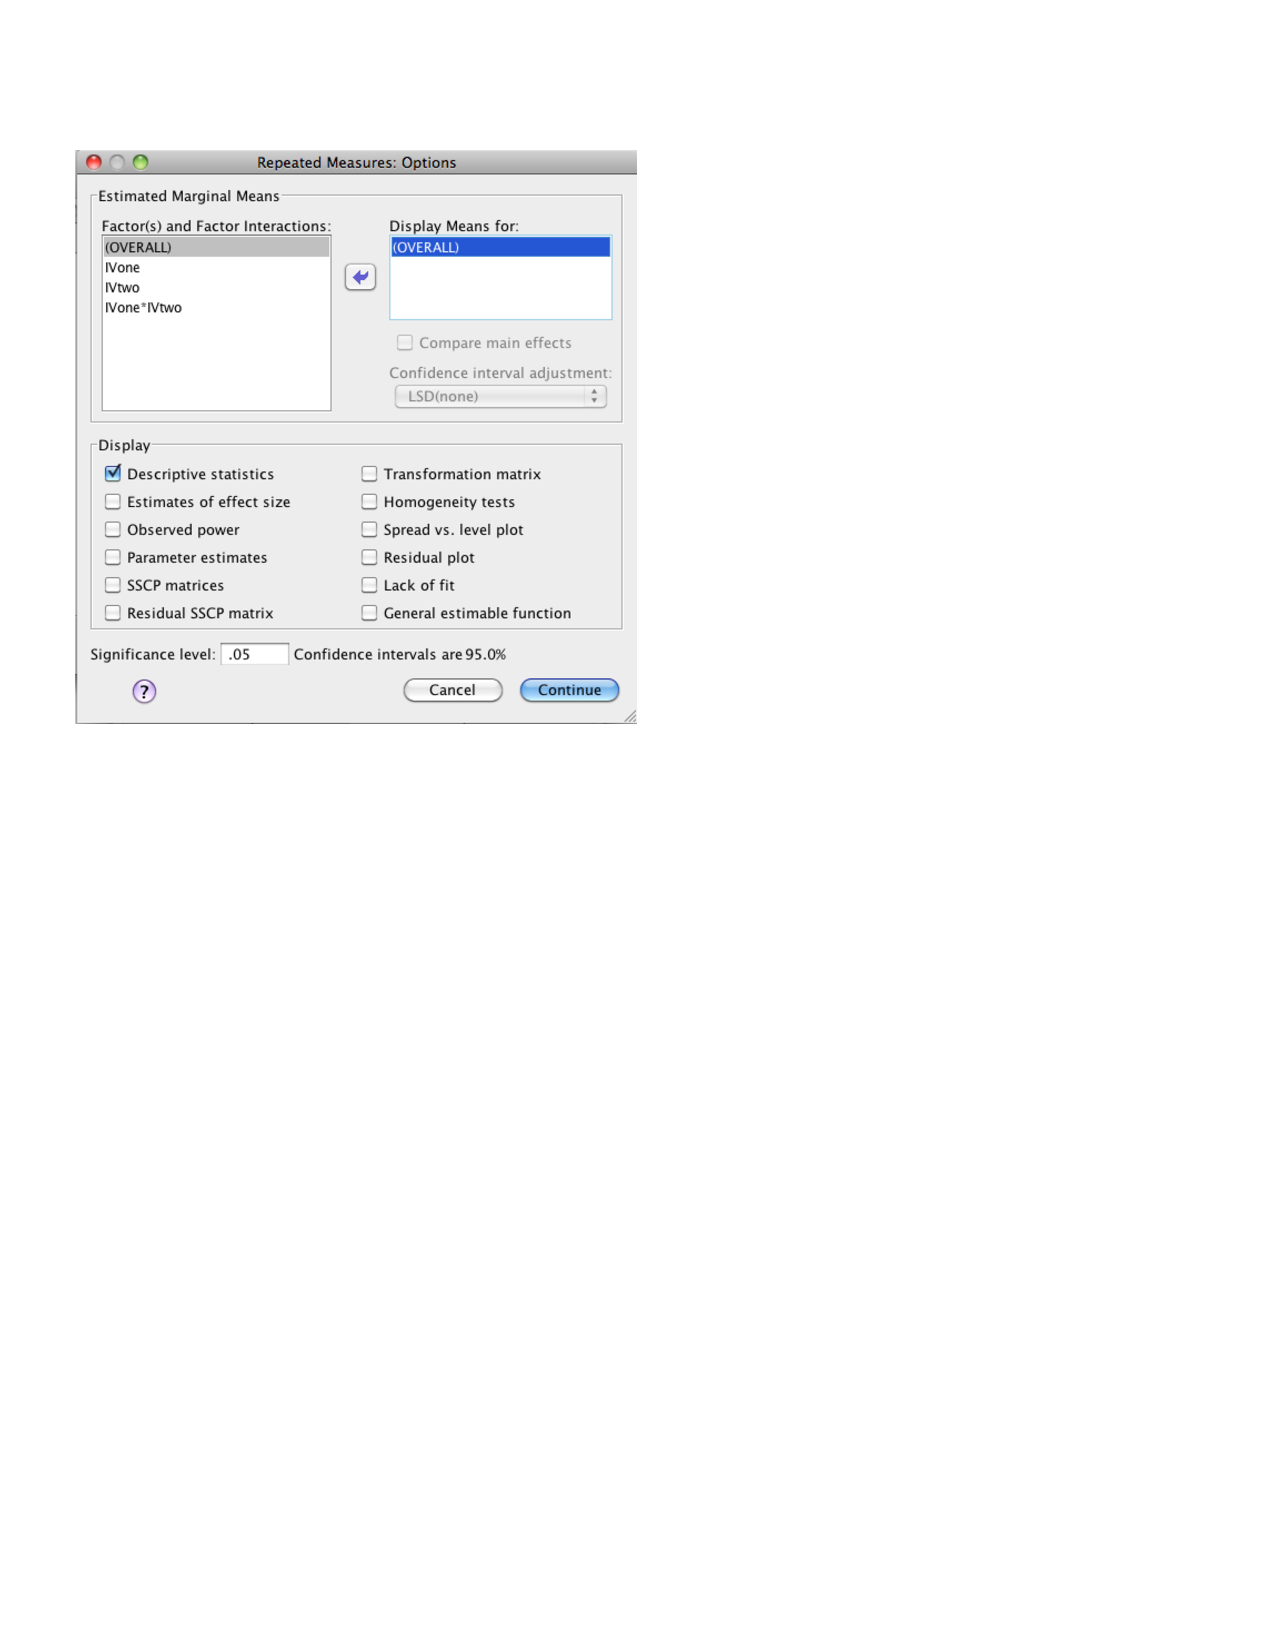
\includegraphics[width=\linewidth]{LabmanualFigures/SPSS11.pdf}
      \caption{Option to report descriptive statistics}
      \label{fig:SPSS11}
\end{figure}

\subsection{Finding numbers in the SPSS analysis output}

SPSS gives you lots of information, you need to know what you are looking for. When you report the results from a 2x2 ANOVA, you will have 2 main effects, and 1 interaction. This means you will be looking for 3 F-values, 3 MSEs (Mean squared error terms), and 3 associated p-values. You will also need to know the means for the main effects and the means for the interaction.

\begin{figure}
      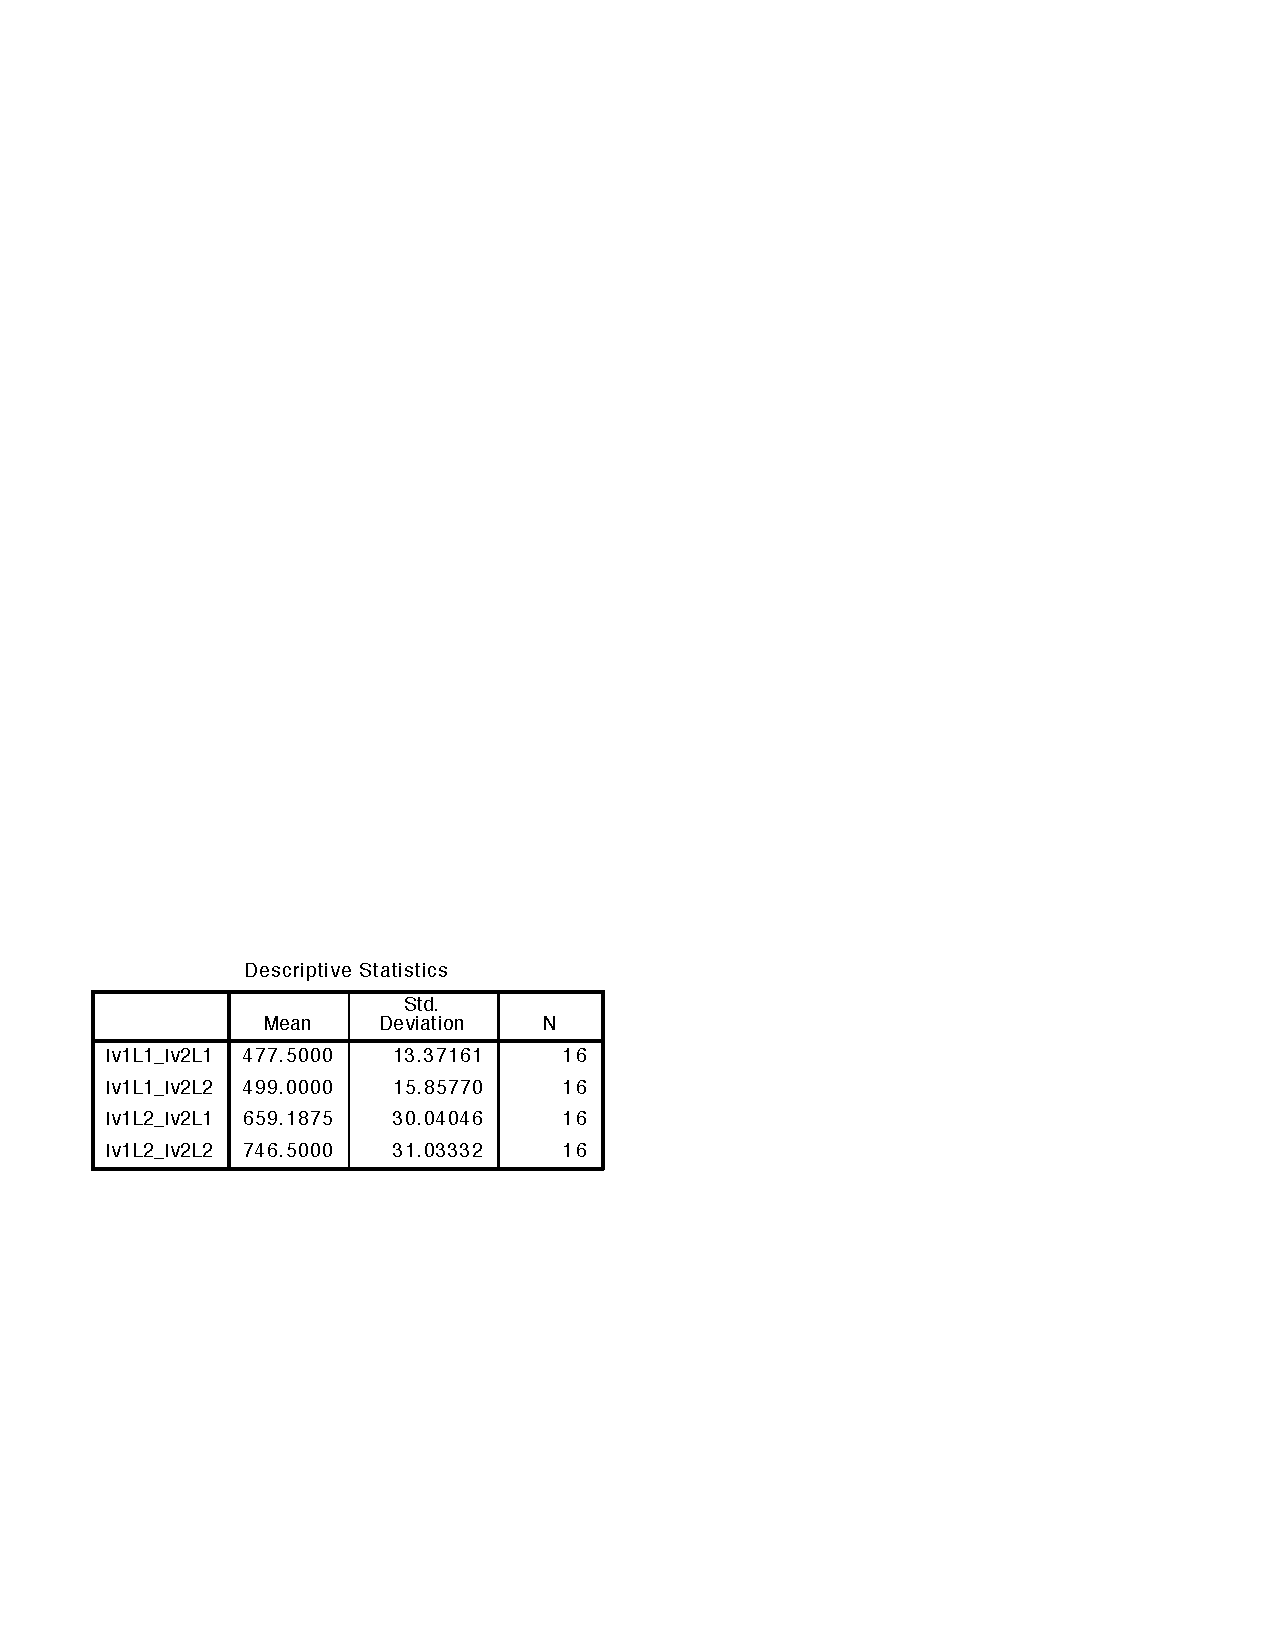
\includegraphics[width=\linewidth]{LabmanualFigures/SPSS12.pdf}
      \caption{Descriptive Statistics}
      \label{fig:SPSS12}
\end{figure}

If you chose the option for descriptive stats, then you will see a small table with Means and standard deviations for each condition in the design. You will use these means to compute averages for the main effects. You will use these means to report the pattern for the interaction.

\subsection{The ANOVA table}
All of the information that you need to report main effects and interactions is available in  the "tests of within-subjects effects" table.

\begin{figure}
      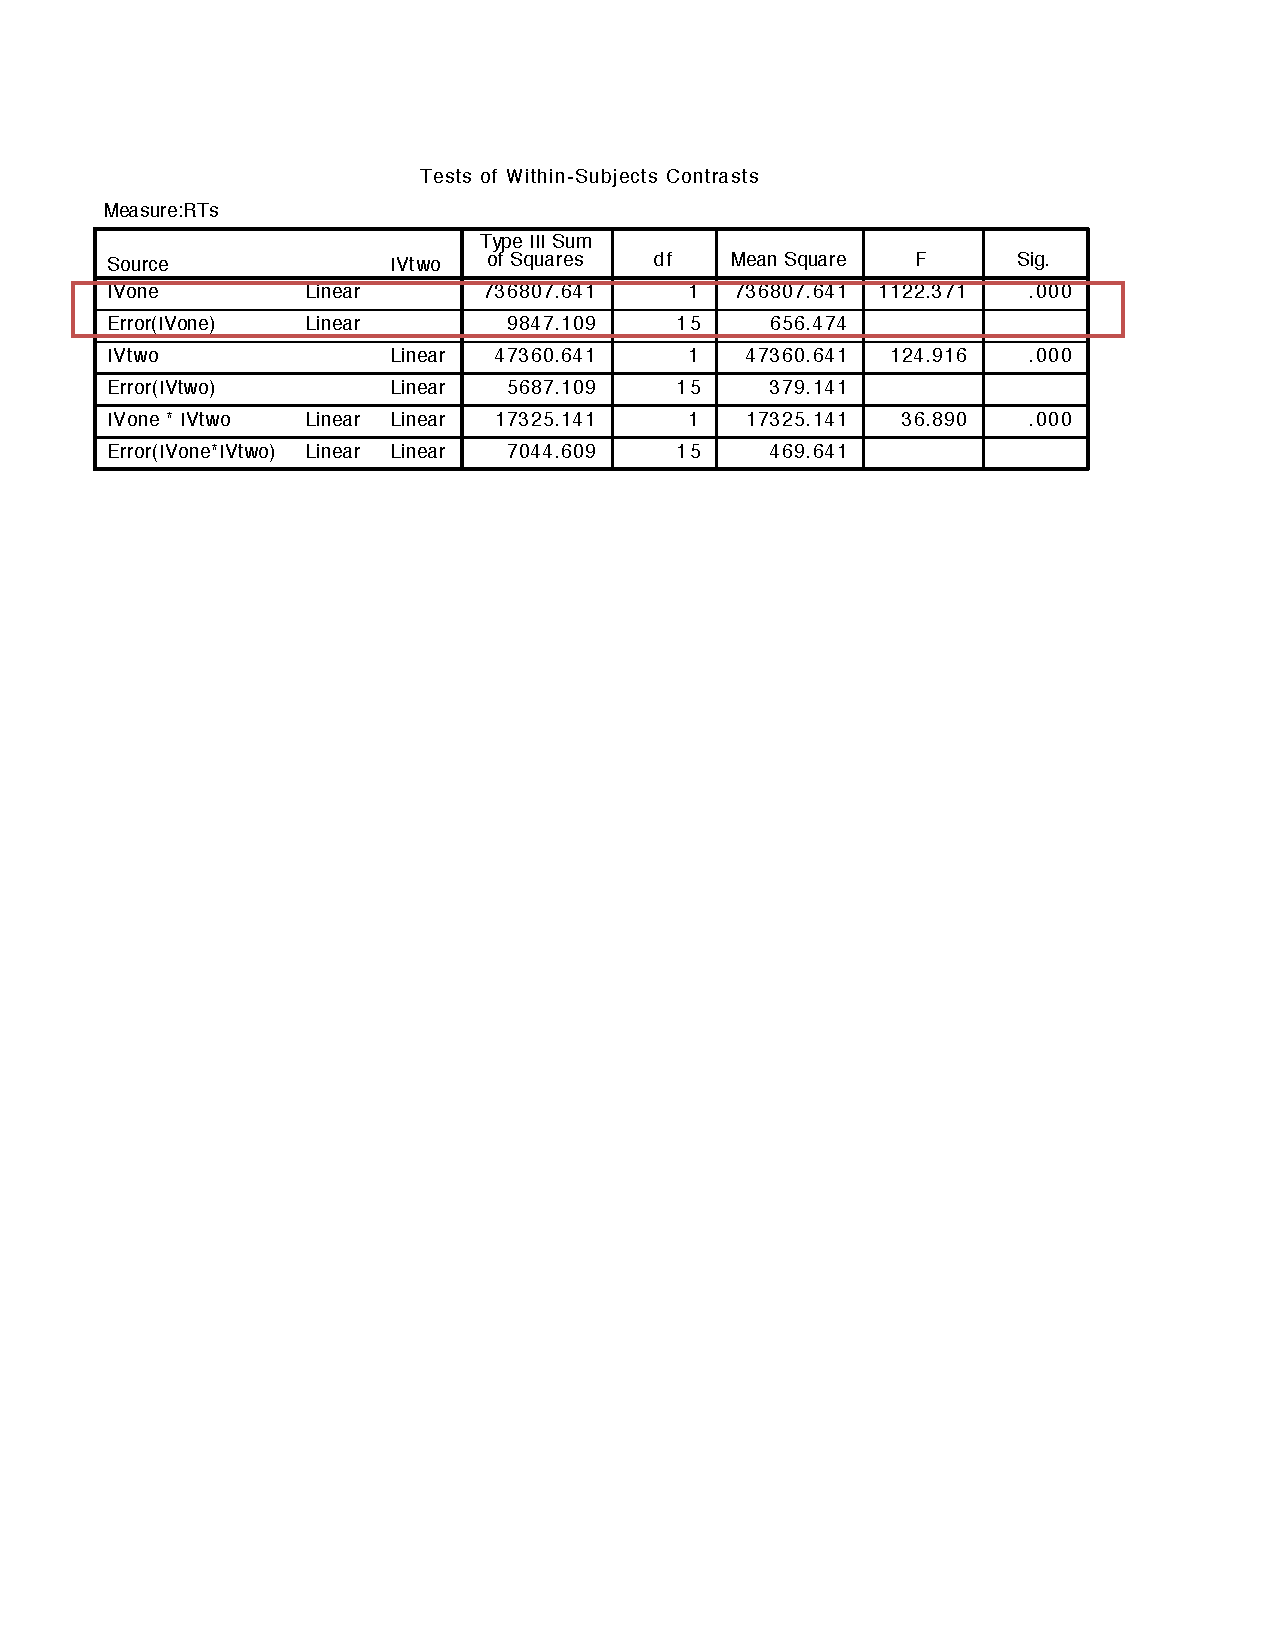
\includegraphics[width=\linewidth]{LabmanualFigures/SPSS13.pdf}
      \caption{ANOVA table}
      \label{fig:SPSS13}
\end{figure}

\subsection{Main effect for IV 1}

Each main effect is listed under source. Each main effect has a corresponding error term listed below. The source for the main effect of independent variable 1 is labeled IV one. You will see it has a corresponding df of 1, an F-value of 112.371, and a p-value <.05. This main effect is significant. You would report this in the following way.

The main effect for independent variable 1 was significant, F(1,15) = 112.371, MSE = 656.47, p<.05. 

The 15 comes from the df from the error term for IVone. As well, the MSE (656.47) comes from the Mean Square from the error term. When you report the main effect, you will also need to report the pattern. The above sentence simply tells the reader that there was a significant difference between the levels of IVone, however it does not explain whether level 1 was larger or smaller than level 2. To report the main effect you will need to compute the averages for each level of IVone. You can do this directly in excel, or you can have SPSS compute these numbers for you by checking the appropriate options before running the analysis. You will need all of the numbers from the above descriptive statistics table. 

First, we find the average for level 1 of IVone (477.5 + 499)/2 = 488

Second, we find the average for level 2 of IVone (659.1875 + 746.5)/2 = 703

Now we can write a complete description of the main effect for IVone. 

The main effect for independent variable 1 was significant, F(1,15) = 112.371, MSE = 656.47, p<.05. Mean performance was lower for level 1 (488) than level 2 (703). 


\subsection{Main effect for IV 2}

Following the same steps as above we look for IV two in the source table and find the dfs, the F-value, the MSE for the error term, and the p-value. 

The main effect for independent variable 2 was significant, F(1,15) = 124.92, MSE = 379.14, p<.05. Mean performance was lower for level 1 (568) than level 2 (623).

\subsection{The interaction effect}

Reporting the interaction uses the same information that you would use to report the main effect. The interaction is listed in the source table as IVone*IVtwo. It has corresponding dfs, F-value, MSE for the error term, and a p-value. 

The interaction between independent variable one and two was significant, F(1,15) = 36.89, MSE = 469.64, p<.05. The difference between level one and level two for independent variable two was smaller for level one (499 - 478 = 21) than level two (747 - 659 = 88) of independent variable 1. 

\subsection{Post Hoc Tests to interpret the interaction}

Post hoc tests are used to clarify the nature of the interaction. In the above example we found a significant interaction. The difference between level 1 and level 2 for IV two was 21 and 88 for level 1 and level 2 of the first independent variable. The significant interaction tells us that 21 and 88 are significantly different from each other. However, we still do not know whether each comparison is significant in an of itself. For example it may be the case that the difference between level 1 and level 2 for IV 2 was only significant for the 2nd level of IV1 (88), and not significant for the 1st level of IV1 (21). In this example you can run a paired t-test, or a one-way repeated measures ANOVA on the specific comparison that you are interested in. For example, you would compare the means from IV1L1/IV2L1 and IV1L1/IV2L2. This comparison would test whether the difference of 21 that was found was actually significant from 0. You will report the statistics for the post-hoc tests in the same manner as you would report t-tests, or F-statistics from the above examples. 

\chapter{Writing An APA Style Paper}
\lhead{\allcaps{Writing an APA style Paper}}
\openepigraph{Memory... is the diary that we all carry about with us.}{---Oscar Wilde}

\section{How to write a research report}

Bean, J. C. (2001). Engaging ideas: The professor’s guide to integrating writing, critical thinking, and active learning in the classroom. San Francisco: Jossey-Bass Publishers

A formal scientific research report is a piece of professional writing addressed to other professionals who are interested in the investigation you conducted. They will want to know why you did the investigation, how you did it, what you found out, and whether your findings were significant and useful. Research reports usually follow a standard five-part format: (1) introduction, (2) methods, (3) results (4) discussion of results, and (5) conclusions and recommendations.

\subsection{Introduction} 
Here you explain briefly the purpose of your investigation. What problem did you address? Why did you address it? You will need to provide enough background to enable the reader to understand the problem being investigated. Sometimes the introduction also includes a “literature review” summarizing previous research addressing the same or a related problem. In many scientific disciplines, it is also conventional to present a hypothesis—a tentative “answer” to the question that your investigation will confirm or disconfirm.

\subsection{Methods} 
This is a “cookbook” section detailing how you did your investigation. It provides enough details so that other researchers could replicate your investigation. Usually, this section includes the following subsections: (a) research design, (b) apparatus and materials, and (c) procedures followed.

\subsection{Results} 
This section sometimes headed “Findings,” presents the empirical results of your investigation. Often, your findings are displayed in figures, tables, graphs, or charts that are referenced in the text. Even though the data are displayed in visuals, the text itself should also describe the most significant data. (Imagine that the figures are displayed on a view graph and that you are explaining them orally, using a pointer. Your written text should transcribe what you would say orally.) Your figures and tables must have sufficient information to stand along, including accurate titles and clear labels for all meaning-carrying features.

\subsection{Discussion of results} 
This is the main part of the report, the part that will be read with the most care by other professionals. Here you explain the significance of your findings by relating what you discovered to the problem you set out to investigate in your introduction. Did your investigation accomplish your purpose? Did it answer your questions? Did it confirm or disconfirm your hypothesis? Are you results useful? Why or why not? Did you discover information that you hadn’t anticipated? Was your research design appropriate? Did your investigation raise new questions? Are there implications from your results that need to be explored? The key to success in this section is to link your findings to the questions and problems raised in the introduction.

\subsection{Conclusions and recommendations} 
In this last section, you focus on the main things you learned from the investigation and, in some cases, on the practical applications of your investigation. If your investigation was a pure research project, this section can be a summary of your most important findings along with recommendations for further research. If your investigation was aimed at making a practical decision (for example, an engineering design decisions), here you recommend appropriate actions. What you say in this section depends on the context of your investigation and the expectations of your readers.

\section{APA style}

The next sections provide information about APA style, and an example research report written in APA style.

\subsection{APA style formatting}

\includepdf[pages=1-6]{APA1.pdf}

\subsection{Sample APA report}

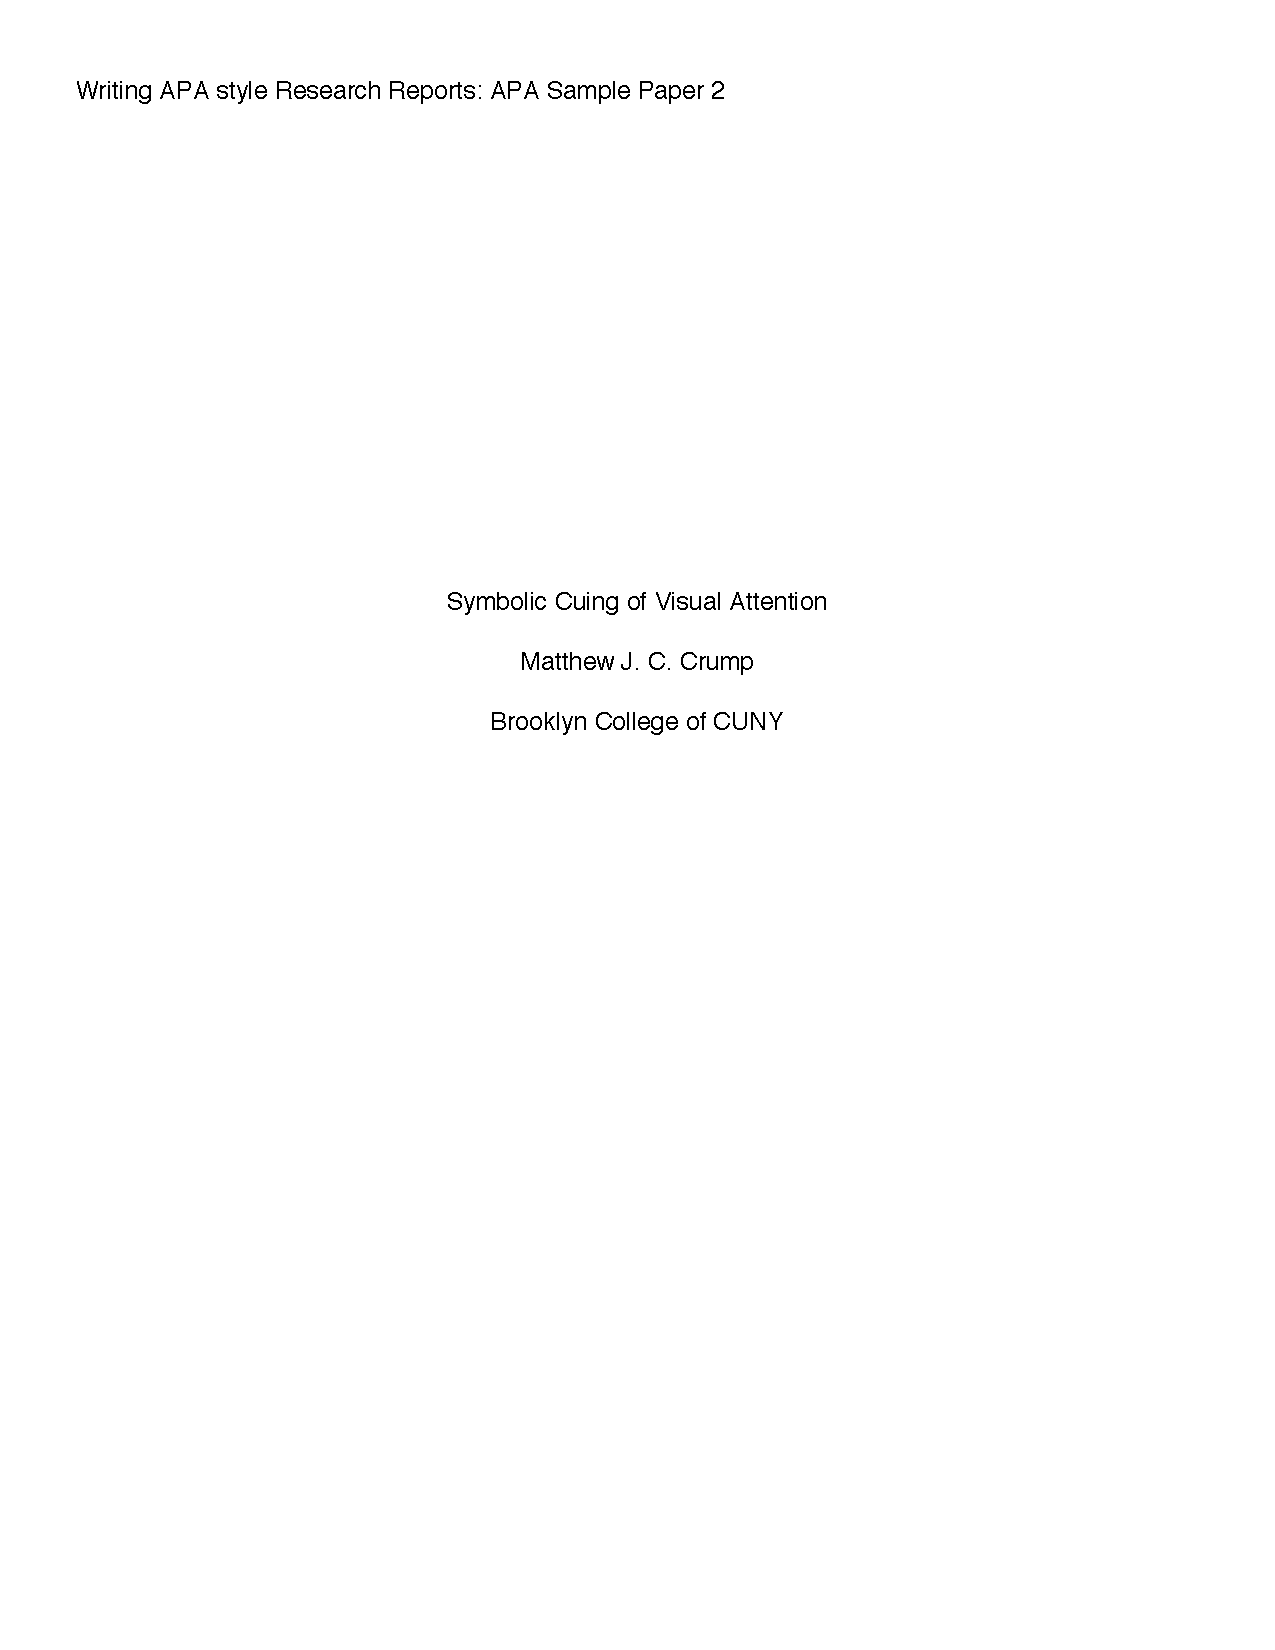
\includepdf[pages=1-8]{APA2.pdf}




\bibliography{mybib}
\bibliographystyle{apalike}

\printindex
\end{document}
